
\documentclass[notoc,nofonts,a4paper,twoside,nobib]{tufte-book}
%\documentclass[nofonts,a4paper,twoside]{book}

\usepackage{currfile,hyperxmp}

\usepackage{filemod}
   
\usepackage[
    type={CC},
    modifier={by-sa},
    version={4.0},
    imagewidth = 17mm,
 ]{doclicense}


\usepackage[refsegment=chapter,style=authoryear-comp,natbib=true]{biblatex}

\addbibresource{literature.bib}



\usepackage{amssymb,amsmath}



\usepackage{tikz,tikz-3dplot}



\newcommand{\inputtikz}[1]{%

 \tikzexternalenable
  \tikzsetnextfilename{#1}%
  \input{#1.tikz}%
  \tikzexternaldisable

}


\usetikzlibrary{math,matrix,fit,positioning,intersections}
\usetikzlibrary{patterns,decorations.pathmorphing,decorations.markings}

\usetikzlibrary{calc}
\usetikzlibrary{arrows.meta} %needed tikz library

\usepackage{standalone}
\usepackage{pgfplots}
 \pgfplotsset{compat=newest}
\usepgfplotslibrary{groupplots}

\tikzset{>=latex}

\usepackage{tikzorbital}
 \usepackage{tikzsymbols}
\usetikzlibrary{quotes,angles}

\usepackage{currfile,hyperxmp}


\pgfplotsset{
tufte line/.style={
    axis line style={draw opacity=0},
    ytick=\empty,
    axis x line*=bottom,
    x axis line style={
      draw opacity=1,
      gray,
      thick
},
 %   yticklabel=\pgfmathprintnumber{\tick}
  }
  }

\tikzset{
mymat/.style={
    matrix of math nodes,
    left delimiter=|, right delimiter=|,
    align=center,
    column sep=-\pgflinewidth,
}
%,mymats/.style={
%    mymat,
%    nodes={draw,fill=#1}
%} 
 }
 
\newcommand{\myarrow}[5]{\draw[#4](#1.south -| #2)  -- ++(#3 :6mm) node[above,pos=0.55]{$#5$};
} 

\newcommand{\interactLp}[3]{\myarrow{#1-#2-1}{#1.west}{-135}{<-}{#3}} 
\newcommand{\interactLm}[3]{\myarrow{#1-#2-1}{#1.west}{+135}{->}{#3}} 
\newcommand{\interactRp}[3]{\myarrow{#1-#2-2}{#1.east}{ -45}{<-}{#3}} 
\newcommand{\interactRm}[3]{\myarrow{#1-#2-2}{#1.east}{ +45}{->}{#3}}  

\newcommand{\interactout}[2]{\myarrow{#1-1-1}{#1.west}{+135}{->,dashed}{#2}} 


\newcommand{\benzene}[8]{%
\tikzmath{\x1 = #1; \dx1 = 0.5; \dx2 = 0.9; \ps=0.5;}
\tikzmath{\x2 = \x1 + \dx1 ;}
\tikzmath{\x3 = \x2 + \dx2 ;}
\tikzmath{\x4 = \x3 + \dx1 ;}

\tikzmath{\y1 = #2; \dy = 0.5;}
\tikzmath{\y2 = \y1 + \dy ;}
\tikzmath{\y3 = \y2 + \dy ;}

\orbital[pos = {(\x1,\y2)},scale=#3 * \ps]{pz}
\orbital[pos = {(\x2,\y1)},scale=#4 * \ps]{pz}
\orbital[pos = {(\x3,\y1)},scale=#5 * \ps]{pz}
\orbital[pos = {(\x4,\y2)},scale=#6 * \ps]{pz}
\orbital[pos = {(\x3,\y3)},scale=#7 * \ps]{pz}
\orbital[pos = {(\x2,\y3)},scale=#8 * \ps]{pz}

\draw (\x1,\y2) -- (\x2,\y1) -- (\x3,\y1) -- (\x4,\y2) --(\x3,\y3) 
-- (\x2,\y3) -- (\x1,\y2);
}



\usetikzlibrary{external}
\tikzexternalize[prefix=figures/]



\usepackage[T1]{fontenc}
\usepackage[utf8]{inputenc}


\usepackage{graphicx}
\setkeys{Gin}{width=\linewidth,totalheight=\textheight,keepaspectratio}


\usepackage{booktabs}
\usepackage{url}
\usepackage{hyperref}

\usepackage{units}

\usepackage{chemformula}

\usepackage{braket}
\setcounter{secnumdepth}{0}

% citations
%\usepackage{natbib}
%\bibliographystyle{plainnat}
%\setcitestyle{round} 

% pandoc syntax highlighting
%\usepackage{color}
%\usepackage{fancyvrb}



% longtable
\usepackage{longtable,booktabs}
\usepackage{multicol}
\usepackage[normalem]{ulem}

% morefloats
\usepackage{morefloats}

\usepackage{calc}




%% -- tint overrides
%% fonts, using roboto (condensed) as default
\usepackage[sfdefault,condensed]{roboto}
%% also nice: \usepackage[default]{lato}

%% colored links, setting 'borrowed' from RJournal.sty with 'Thanks, Achim!'
\RequirePackage{color}
\definecolor{link}{rgb}{0.1,0.1,0.8} %% blue with some grey
\hypersetup{
  colorlinks,%
  citecolor=link,%
  filecolor=link,%
  linkcolor=link,%
  urlcolor=link
}

%% macros
\makeatletter

%% -- tint does not use italics or allcaps in title
\renewcommand{\maketitle}{%     
  \newpage
  \global\@topnum\z@% prevent floats from being placed at the top of the page
  \begingroup
    \setlength{\parindent}{0pt}%
    \setlength{\parskip}{4pt}%
    \let\@@title\@empty
    \let\@@author\@empty
    \let\@@date\@empty
    \ifthenelse{\boolean{@tufte@sfsidenotes}}{%
      %\gdef\@@title{\sffamily\LARGE\allcaps{\@title}\par}%
      %\gdef\@@author{\sffamily\Large\allcaps{\@author}\par}%
      %\gdef\@@date{\sffamily\Large\allcaps{\@date}\par}%
      \gdef\@@title{\begingroup\fontseries{b}\selectfont\LARGE{\@title}\par}%
      \gdef\@@author{\begingroup\fontseries{l}\selectfont\Large{\@author}\par}%
      \gdef\@@date{\begingroup\fontseries{l}\selectfont\Large{\@date}\par}%
    }{%
      %\gdef\@@title{\LARGE\itshape\@title\par}%
      %\gdef\@@author{\Large\itshape\@author\par}%
      %\gdef\@@date{\Large\itshape\@date\par}%
      %\gdef\@@title{\begingroup\fontseries{b}\selectfont\LARGE\@title\par\endgroup}%
      %\gdef\@@author{\begingroup\fontseries{l}\selectfont\Large\@author\par\endgroup}%
      %\gdef\@@date{\begingroup\fontseries{l}\selectfont\Large\@date\par\endgroup}%
      \gdef\@@title{\begingroup\fontseries{b}\fontsize{28}{60}\selectfont\@title\par\endgroup}%
      \gdef\@@author{\begingroup\fontseries{l}\fontsize{16}{20}\selectfont\@author\par\endgroup}%
      \gdef\@@date{\begingroup\fontseries{l}\fontsize{16}{20}\selectfont\@date\par\endgroup}%
    }%
    %\phantom{XXX}%
    \vspace{12pc}%
    \@@title%
    \vspace{4pc}%
    \@@author
    \@@date
  \endgroup
  \thispagestyle{plain}% suppress the running head
  \tuftebreak% add some space before the text begins
  \@afterindentfalse\@afterheading% suppress indentation of the next paragraph
}

%% -- tint does not use italics or allcaps in section/subsection/paragraph
\titleformat{\chapter}%
  [display]% shape
  {\relax\ifthenelse{\NOT\boolean{@tufte@symmetric}}{\begin{fullwidth}}{}}% format applied to label+text
  %{\itshape\huge\thechapter}% label
  {\huge Chapter \thechapter}% label
  {0pt}% horizontal separation between label and title body
  %{\huge\rmfamily\itshape}% before the title body
  {\fontseries{b}\selectfont\huge}% before the title body
  [\ifthenelse{\NOT\boolean{@tufte@symmetric}}{\end{fullwidth}}{}]% after the title body

\titleformat{\section}%
  [hang]% shape
  %{\normalfont\Large\itshape}% format applied to label+text
  {\fontseries{b}\selectfont\Large}% format applied to label+text
  {\thesection}% label
  {1em}% horizontal separation between label and title body
  {}% before the title body
  []% after the title body

\titleformat{\subsection}%
  [hang]% shape
  %{\normalfont\large\itshape}% format applied to label+text
  {\fontseries{m}\selectfont\large}% format applied to label+text
  {\thesubsection}% label
  {1em}% horizontal separation between label and title body
  {}% before the title body
  []% after the title body

\titleformat{\paragraph}%
  [runin]% shape
  %{\normalfont\itshape}% format applied to label+text
  {\fontseries{l}\selectfont}% format applied to label+text
  {\theparagraph}% label
  {1em}% horizontal separation between label and title body
  {}% before the title body
  []% after the title body

%% -- tint does not use italics here either
% Formatting for main TOC (printed in front matter)
% {section} [left] {above} {before w/label} {before w/o label} {filler + page} [after]
\ifthenelse{\boolean{@tufte@toc}}{%
  \titlecontents{part}% FIXME
    [0em] % distance from left margin
    %{\vspace{1.5\baselineskip}\begin{fullwidth}\LARGE\rmfamily\itshape} % above (global formatting of entry)
    {\vspace{1.5\baselineskip}\begin{fullwidth}\fontseries{m}\selectfont\LARGE} % above (global formatting of entry)
    {\contentslabel{2em}} % before w/label (label = ``II'')
    {} % before w/o label
    {\rmfamily\upshape\qquad\thecontentspage} % filler + page (leaders and page num)
    [\end{fullwidth}] % after
  \titlecontents{chapter}%
    [0em] % distance from left margin
    %{\vspace{1.5\baselineskip}\begin{fullwidth}\LARGE\rmfamily\itshape} % above (global formatting of entry)
    {\vspace{1.5\baselineskip}\begin{fullwidth}\fontseries{m}\selectfont\LARGE} % above (global formatting of entry)
    {\hspace*{0em}\contentslabel{2em}} % before w/label (label = ``2'')
    {\hspace*{0em}} % before w/o label
    %{\rmfamily\upshape\qquad\thecontentspage} % filler + page (leaders and page num)
    {\upshape\qquad\thecontentspage} % filler + page (leaders and page num)
    [\end{fullwidth}] % after
  \titlecontents{section}% FIXME
    [0em] % distance from left margin
    %{\vspace{0\baselineskip}\begin{fullwidth}\Large\rmfamily\itshape} % above (global formatting of entry)
    {\vspace{0\baselineskip}\begin{fullwidth}\fontseries{m}\selectfont\Large} % above (global formatting of entry)
    {\hspace*{2em}\contentslabel{2em}} % before w/label (label = ``2.6'')
    {\hspace*{2em}} % before w/o label
    %{\rmfamily\upshape\qquad\thecontentspage} % filler + page (leaders and page num)
    {\upshape\qquad\thecontentspage} % filler + page (leaders and page num)
    [\end{fullwidth}] % after
  \titlecontents{subsection}% FIXME
    [0em] % distance from left margin
    %{\vspace{0\baselineskip}\begin{fullwidth}\large\rmfamily\itshape} % above (global formatting of entry)
    {\vspace{0\baselineskip}\begin{fullwidth}\fontseries{m}\selectfont\large} % above (global formatting of entry)
    {\hspace*{4em}\contentslabel{4em}} % before w/label (label = ``2.6.1'')
    {\hspace*{4em}} % before w/o label
    %{\rmfamily\upshape\qquad\thecontentspage} % filler + page (leaders and page num)
    {\upshape\qquad\thecontentspage} % filler + page (leaders and page num)
    [\end{fullwidth}] % after
  \titlecontents{paragraph}% FIXME
    [0em] % distance from left margin
    %{\vspace{0\baselineskip}\begin{fullwidth}\normalsize\rmfamily\itshape} % above (global formatting of entry)
    {\vspace{0\baselineskip}\begin{fullwidth}\fontseries{m}\selectfont\normalsize\rmfamily} % above (global formatting of entry)
    {\hspace*{6em}\contentslabel{2em}} % before w/label (label = ``2.6.0.0.1'')
    {\hspace*{6em}} % before w/o label
    %{\rmfamily\upshape\qquad\thecontentspage} % filler + page (leaders and page num)
    {\upshape\qquad\thecontentspage} % filler + page (leaders and page num)
    [\end{fullwidth}] % after
}{}

% tint: no smallcaps in header 
% The 'fancy' page style is the default style for all pages.
\fancyhf{} % clear header and footer fields
\ifthenelse{\boolean{@tufte@twoside}}
  %{\fancyhead[LE]{\thepage\quad\smallcaps{\newlinetospace{\plainauthor}}}%
  %  \fancyhead[RO]{\smallcaps{\newlinetospace{\plaintitle}}\quad\thepage}}
  %{\fancyhead[RE,RO]{\smallcaps{\newlinetospace{\plaintitle}}\quad\thepage}}
  {\fancyhead[LE]{\thepage\quad{\newlinetospace{\plaintitle}}}%
    \fancyhead[RO]{{\newlinetospace{\plaintitle}}\quad\thepage}}%
  {\fancyhead[RE,RO]{{\newlinetospace{\plaintitle}}\quad\thepage}}
  



\makeatother



\renewcommand{\chaptermark}[1]{\markboth{#1}{}}%


\ifthenelse{\boolean{@tufte@twoside}}
  {\fancyhead[LE]{\thepage\quad{\newlinetospace{Experiments in Spectroscopy}}}%
    \fancyhead[RO]{{\newlinetospace{\leftmark}}\quad\thepage}}%
  {\fancyhead[RE,RO]{{\newlinetospace{c}}\quad\thepage}}
  
 
%\makeatletter
\fancypagestyle{mystyle}{%
\fancyhf{}%
\fancyfoot[L]{%
\begin{minipage}{17mm}
\doclicenseImage
\end{minipage}
\begin{minipage}{60mm}
 \footnotesize
 \doclicenseLongText
\end{minipage}%
}% 
%\fancyfoot[L]{\doclicenseThis}% 
}
%\makeatother

\usepackage{etoolbox}
\patchcmd{\chapter}{\thispagestyle{plain}}{\thispagestyle{mystyle}}{}{}



\hypersetup{
 linktocpage,
  colorlinks,
  citecolor=Maroon,
  filecolor=Maroon,
  linkcolor=RoyalBlue,
  urlcolor=RoyalBlue
}

\newcommand{\chapterauthors}{Markus Lippitz}
\newcommand{\lastmod}{\Filemodtoday{\currfilepath}}


\newcommand{\addtochapter}{%
\vspace*{-12mm}{
\setlength{\parindent}{0pt}
\chapterauthors \newline \lastmod
}
\vspace*{12mm}
}

\makeatletter
\let\stdchapter\chapter
\renewcommand*\chapter{%
  \@ifstar{\starchapter}{\@dblarg\nostarchapter}}
\newcommand*\starchapter[1]{\stdchapter*{#1}}
\def\nostarchapter[#1]#2{\stdchapter[{#1}]{#2} \addtochapter}
\makeatother

\makeatletter
  \def\my@tag@font{\scriptsize}
  \def\maketag@@@#1{\hbox{\m@th\normalfont\color{gray}\my@tag@font#1}}
  \let\amsmath@eqref\eqref
  \renewcommand\eqref[1]{{\let\my@tag@font\relax\amsmath@eqref{#1}}}
\makeatother

%\includeonly{1_fundamentals/1_absorption/absorption}
%\includeonly{1_fundamentals/2_fluorescence/fluorescence}


\begin{document}
  \tikzexternaldisable


\title{Experiments in Spectroscopy}

\author{Markus Lippitz}
\date{\today}
%\date{July 21, 2020}


\maketitle


%
\tableofcontents

%\renewcommand{\lastmod}{\ \ }
\renewcommand{\chapterauthors}{\ \ }

\chapter*{Preface}


These are the lecture notes of my lecture on optical spectroscopy, given in the first corona semester in summer 2020. It aims at students in the first year of the master's program, but should be accessible also to students in the last year of the bachelor's program. You need some quantum mechanics and an introduction to the physics of molecules.

The idea of this lecture was to focus on \emph{experiments}. Each chapter is build around an experiment and tries to explain everything that is needed to appreciate that experiment. As I am convinced that one only understands something if one really has worked with the concepts, each chapter has a \emph{task}, which is in many cases to evaluate 'real' experimental data, or to simulate the experiment in a computer. The chapters are rather independent of each other, although the order has some sense. One thus can choose appealing chapters and skip others.

In the corona semester, I handed out these lecture notes to the students and prepared short (approx. 15 minutes) introductory videos to each chapter. I have the impression that it is easier for me to put things into context when talking then when writing, as I dare to be more sloppy. I did not enforce any timing, any rhythm during the semester. Everyone could select his or her pace and choice of chapters. During live video conferences, we discussed open questions and the results of the students work on the tasks\sidenote{The tasks were also uploaded on the elearning platform and visible to all others who have completed a task.}.

These notes are 'work in progress', and probably never really finished. If you find mistakes, please tell me. I am also always interested in other sources covering these topics.
The most current version of the lecture notes can be found at 
\href{http://www.ep3.uni-bayreuth.de/lecturenotes}{my website}. There I link also the material for the tasks and the videos. I have put everything under a CC-BY-SA license (see footer). In my words: feel free to do with it whatever you like. If you make your work available to the public, mention me and use a similar license. 


The lecture notes are typeset using the LaTeX class 'tufte-book' by Bil Kleb, Bill Wood, and Kevin Godby\sidenote{\href{https://tufte-latex.github.io/tufte-latex/}{tufte-latex}}, which  approximates the work of Edward Tufte\sidenote{\href{https://www.edwardtufte.com/}{edwardtufte.com}}. I applied many of the modifications introduced by Dirk Eddelbuettel in the 'tint' R package\sidenote{\href{https://dirk.eddelbuettel.com/code/tint.html}{tint: Tint is not Tufte}}. For the time being, the source is LaTeX, not markdown.

\vspace{2\baselineskip}

Markus Lippitz \\ Bayreuth, July 17, 2020



%
\part{Fundamentals}

%\renewcommand{\lastmod}{April 29, 2020}

\chapter{Absorption}




\section{Tasks}

\begin{itemize}
\item Get acquainted with the different measures for absorption and how they relate. Starting from the experimental values in the following papers, calculate all other measures.

\begin{tabular}{ll}
InGaAs quantum dots & \cite{Borri:2002p139}, last page  \\
CdSe nanocrystals & \cite{Jasieniak:2009er}, Fig. 2 and 3 \\
xanthene dye & \cite{Kastrup:2004p1737}, Fig. 4d   \\
MEH-PPV conjugated polymer  & \cite{Hou:2017jm}, Fig. 3 \\
\end{tabular}


\item Get a feeling for typical absolute values and compare them to relevant  other quantities, such as geometrical size, bond lengths, transition rates etc. Sometimes it makes sense to factor out some constants and compare only then.
\item Why are there so many different measures for absorption? Find use cases where it makes especially sense to use one measure and not the others.

\end{itemize}







%\section{Experiment}
\section{Experimental technique}

An UV/VIS spectrometer measures the  power $P$ transmitted through a cuvette of optical path length $L$ and compares it to the power $P_0$ in a reference path. In most cases, also here, the reference path holds a cuvette containing  the plain solvent. The transmission $T = P / P_0$ is converted into the absorbance $A = - \log_{10} T = - \log_{10} ( P / P_0)$. The data set gives absorbance as function of wavelength.

\begin{marginfigure}
\inputtikz{\currfiledir uvvis}
\caption{Sketch of a UV/VIS spectrometer}
\end{marginfigure}



Grating spectrometers use an entrance slit to define the spectral resolution $d \lambda$, which is independent of the actual wavelength $\lambda$, as can be seen when inspecting the   angular dispersion relation of a grating. Due to the reciprocal relation between wavelength and frequency or energy, the spectral resolution in units of energy $d \nu$ is not constant anymore.




\section{Lambert-Beer law and the absorption coefficient}

The transmitted power drops exponentially with  concentration $C$ and  path length $L$
\begin{equation}
 P = P_0 \, 10^{- \epsilon\, C \, L}
\end{equation}
where $\epsilon$ is the (decadic) molar absorption\sidenote{The difference between abortion and extinction will be discussed elsewhere.} coefficient. We stick here to a base of $10$, 
so that the absorbance or optical density equals 
\begin{equation}
 A = \epsilon\, C \, L \quad.
\end{equation}
However, similar definitions with a base of $e$ are used sometimes. Our choice leads to the appearance of factors of $\ln(10)$ every now and then. The concentration is typically given as molarity (1 M = 1 mol/l), and lengths for practical reasons in centimeter
so that the molar absorption coefficient has the unit 1/(M  cm). As we are concerned with spectroscopy the molar absorption coefficient $\epsilon$ depends of course on the wavelength or frequency of light.

\section{Absorption cross section}


The interaction cross section $\sigma$ of a process is an imagined area around the particle, which, when hit by a photon, triggers the considered process. When a photon hits on the absorption cross section $\sigma_{\text{abs}}$ of a molecule it will be absorbed. If it does not hit it will pass unperturbed. All details of the physics are summarized in the area, which makes it easy to relate the absorption cross section with the absorbance. 
\begin{marginfigure}
\inputtikz{\currfiledir crosssection}
\caption{Sketch  disks hit by rays}
\end{marginfigure}


We consider randomly arranged molecules of molar concentration $C$ in a thin slab of thickness $dx$. The probability that a photon is absorbed in this slab is
\begin{equation}
 1 - T =1 -  10^{- \epsilon\, C \, dx} \approx \ln (10) \; \epsilon\, C \, dx \quad .
\end{equation}
In comparison, when each molecule has an absorption cross section $\sigma_{\text{abs}}$, we get an absorption probability 
\begin{equation}
 1 - T = \sigma_{\text{abs}} \, C \, N_A \, dx
\end{equation}
where $N_A = 6.022 \cdot 10^{23}$~{1/mol} is the Avogadro number.  We also made the Born approximation, i.e., that multiple interactions can be neglected, or the absorption cross sections do not overlap, which is equivalent to the approximation made above to remove the exponential function.  We thus find
\begin{equation}
 \sigma_{\text{abs}}(\omega) =  \frac{\ln(10)}{ N_A } \, \epsilon(\omega)
\end{equation}
which has the unit of an area. As the  molar absorption coefficient $\epsilon$  also the absorption cross section $\sigma_{\text{abs}}$ depends on the wavelength of light. If no wavelength is given, the value at the peak of the spectrum is meant.


\section{Lorentz oscillator and oscillator strength}


\begin{marginfigure}
\inputtikz{\currfiledir mass_spring}
\caption{A Lorentz oscillator}
\end{marginfigure}


The Lorentz oscillator is a simple classical model to describe the interaction of light and matter. A mass $m$ of charge $+e$ is connected to a spring. The oscillator has an angular eigen-frequency $\omega_0$ and a damping $\gamma$. It is driven by an external electrical field $E(t) = E_0 \exp(i \omega t)$. The differential equation for the position $x$ reads
\begin{equation}
  \ddot{x} + 2  \gamma  \dot{x} + \omega_0^2 x =  \frac{e}{m} E_0 e^{i \omega t}
\end{equation}
This results in a steady-state solution of \sidenote{check: should be $-i\gamma$ for Lorentz osci}
\begin{equation}
  x(t) = \frac{e}{m}  \frac{1}{\omega_0^2 - \omega^2 + 2  i \gamma \omega } \, E_0 e^{i \omega t} 
\end{equation}
In the case of small damping ($\gamma \ll \omega_0$) this simplifies near the resonance ($\omega \approx \omega_0$) to
\begin{equation}
  x(t) \approx \frac{e}{2 m \omega_0}  \frac{1}{\omega_0 - \omega + i \gamma } \, E_0 e^{i \omega t} 
\end{equation}
The time-averaged power  that the damped oscillator takes out of the driving force $F(t) = e E(t)$ can be calculated in this approximation as
%
\begin{eqnarray}
 P_{\text{abs}} &= &  - \frac{1}{T} \int_0^T F \, \frac{ds}{dt} \, dt =  
  - \frac{1}{T}  \int_0^T Re \left\{  e E(t) \right\}  \, Re \left\{ \dot{x}(t) \right\} \, dt \\
  & = & - Re \left\{i \omega  \frac{e^2  E_0^2 }{2 m \omega_0}  \frac{1}{\omega_0 - \omega +  i \gamma } \right\}  \,   \frac{1}{T}  \int_0^T \left( \cos \omega t \right)^2 dt \\
 % 
%
% P_{\text{abs}} &= & \left< Re \left\{ e E(t) \, \dot{x}(t) \right\} \right> = 
 %
 % & = & Re \left\{ \frac{i \omega}{2} \frac{e^2  E_0^2 }{2 m \omega_0}  \frac{1}{\omega_0 - \omega +  i \gamma } \right\}  \\
%& \approx & Im \left( \frac{e^2  E_0^2 }{4 m }  \frac{1}{\omega_0 - \omega + i \gamma }  \right)
& = & \frac{e^2 E_0^2  }{4 m }  \frac{\gamma }{(\omega_0 - \omega)^2 +  \gamma ^2}  \\
&  = &  \frac{e^2  }{2 \epsilon_0 \, m \,c }  \frac{\gamma }{(\omega_0 - \omega)^2 +  \gamma ^2}  \, |S|  \quad .
\end{eqnarray}
%
The time average has produced a factor of $1/2$ and in the last step we have used the definition of the amplitude of the Poynting vector $|S| = \frac{1}{2} \epsilon_0 c |E_0|^2$. 
We thus find an absorption cross section $\sigma_{\text{abs,Lorenz}}$ of the classical Lorentz oscillator
\begin{equation}
 \sigma_{\text{abs, Lorentz}}(\omega) = \frac{ P_{\text{abs}} }{|S| } = \frac{e^2  }{2 \epsilon_0 \,  m \, c}  \frac{\gamma }{(\omega_0 - \omega)^2 +  \gamma ^2} 
\end{equation}

While many optical transitions show a Lorentzian line shape as predicted by the Lorentz oscillator, the peak height of the absorption line deviates. This deviation is cast into an oscillator strength $f$ so that 
\begin{equation}
 \sigma_{\text{abs}}(\omega) =   \frac{e^2  }{2 \epsilon_0 \,  m \, c}  \frac{\gamma  }{(\omega_0 - \omega)^2 +  \gamma ^2}  \, f
\end{equation}

For single electron transitions starting from the same quantum mechanical level, the Thomas–Reiche–Kuhn sum rule states that the sum over all oscillator strength $f$ equals to one. For this reason, one can interpret the oscillator strength  $f$  to some extent  as the number of electrons involved in  the transition, but one has to be careful, as pointed out by Z. Hens \footcite{Hens:2008kr}.

The spectral integral of the absorption cross section is independent of its width $\gamma$ as
\begin{equation}
 \int \sigma_{\text{abs}}(\omega)  \, d \omega =
   \frac{\pi \, e^2  }{2 \epsilon_0 \,  m \, c} \, f
\end{equation}


\section{Transition dipole moment}

\begin{marginfigure}
\inputtikz{\currfiledir tls_absorption}
\caption{A light beam induces a transition from $\ket{i}$ to the  $\ket{f}$.}
\end{marginfigure}

Fermi's Golden Rule gives the transition rate from the initial state $\ket{i}$ to the final state $\ket{f}$ caused by the time-dependent perturbation $H'$ to the stationary Hamilton operator $H_0$ as
\begin{equation}
 \Gamma_{i \rightarrow f} = \frac{2 \pi}{\hbar} \, \left| \bra{f} H' \ket{i} \right|^2 \, \rho(E) \quad ,
\end{equation}
where  $\rho(E) = d n / d E = \rho(\omega) / \hbar$ is the density of final states. The idea is that the initial state  $\ket{i}$ is well known, but the outcome of the interaction $\ket{f}$ might have free parameters, for example the direction of the emitted electron or the mode of the absorbed photon. The density of states   $\rho(E)$ thus can describe either electronic or photonic states, or both.




In general, the interaction of a charged particle with an electromagnetic vector potential $\mathbf{A}$ is described by the perturbation
\begin{equation}
 H' = - \frac{i \hbar e}{m} \, \mathbf{A \cdot \nabla}  \quad .
\end{equation}
As the spatial extent of our wavefunctions is small compared to the wavelength of light, we employ the dipole approximation and assume $\exp( i \mathbf{k \cdot r}) \approx 1$ in the plane-wave description of the vector potential. In this way, the  perturbation operator $H'$ simplifies to\sidenote{see \textcite{bransden_joachain} for details}
\begin{equation}
 H' =  e \, \mathbf{E} (t)  \mathbf{\cdot \, r} =  e \,E_0 \,  \mathbf{\hat{x} \cdot \, r} \, \cos(\omega t) \quad ,
\end{equation}
where $\mathbf{\hat{x}} $ is a unit vector defining the polarization direction of the light field. We simplify further by using the rotating-wave approximation and keeping only co-rotating parts\sidenote{More on this in the chapter on Rabi oscillations and the Bloch sphere.} 
\begin{equation}
 \cos(\omega t)
 = \frac{1}{2} \left( e^{i \omega t}+  e^{-i \omega t} \right)
 \approx  \frac{1}{2}  e^{i \omega t} 
\end{equation}
so that 
\begin{equation}
H' =  \frac{ e \,E_0}{2}  \,  \mathbf{\hat{x} \cdot \, r} \,  e^{i \omega t}  \quad .
\end{equation}
%
 We introduce the transition dipole matrix element $\mu_{if}$ as
\begin{equation}
\mathbf{\mu}_{if} = -e \, \bra{f}    \mathbf{r} \ket{i}  \quad .
\end{equation}
It has the units of an electric dipole moment, i.e., charge times distance, and is the central element of an optical transition in quantum mechanics. For practical reasons, one uses the unit of 1 Debye = 1 electron displaced by 0.208 \AA.
With this the matrix element  becomes
\begin{equation}
\left| \bra{f} H' \ket{i} \right|^2 =  \frac{1}{4} E_0^2  \, |\mathbf{\hat{x}} \cdot \mathbf{\mu}_{if} |^2 \quad .
\end{equation}
Plugging everything into Fermi's Golden Rule, we get
\begin{equation}
 \Gamma_{i \rightarrow f} = \frac{\pi}{2 \hbar^2} \,  E_0^2  \, |\mathbf{\hat{x}} \cdot \mathbf{\mu}_{if} |^2 \, \rho(\omega) \quad .
\end{equation}
Now we have to take into account that we use a incoherent multimode light source.\sidenote{The effect of a coherent single mode source will be investigated in the context of Rabi oscillations.} The electric field $E$ is here an incoherent superposition of  modes with the  spectral energy density $u(\omega)$.\sidenote{see \textcite{CT} and \textcite{Fox}   for details}
The total power is thus
\begin{equation}
 \frac{1}{2} \epsilon_0  \, E_0^2  = \int  u(\omega)  \, d\omega \quad .
\end{equation}
The  transition rate is thus 
\begin{equation}
 \Gamma_{i \rightarrow f} =   \frac{\pi  }{\hbar^2 \epsilon_0}  \, |\mathbf{\hat{x}} \cdot \mathbf{\mu}_{if} |^2 \,
\int u(\omega)  
  \rho(\omega)  d \omega \quad .
\end{equation}
As the atomic transition is narrow compared with the light spectrum, the density of states $\rho(\omega)$ selects the transition frequency $\omega_{if}$ 
\begin{equation}
 \Gamma_{i \rightarrow f} =   \frac{\pi  }{\hbar^2 \epsilon_0}  \, |\mathbf{\hat{x}} \cdot \mathbf{\mu}_{if} |^2 \,
 u(\omega_{if})   \quad .
\end{equation}
As each absorption event takes out a photon of energy $\hbar \omega_{if}$, and the energy density moves with the speed of light $c$ we get an integrated absorption cross section $\sigma_{\parallel}$ 
\begin{equation}
 \int \sigma_{\parallel}(\omega) \, d \omega = \frac{ \hbar \omega_{if} \, \bar{\Gamma}_{i \rightarrow f} }{c \, u(\omega_{if})}  = 
  \frac{\pi \omega_{if}}{ \hbar c \, \epsilon_0} \,
 |\mathbf{\mu}_{if} |^2  \quad . \label{eq:abs_sigma_mu}
\end{equation}
The index ${\parallel} $ is necessary, as we dropped the dot product between the direction of the transition dipole moment $\mathbf{\mu}_{if}$ and the polarization direction $\mathbf{\hat{x}}$, assuming optimal parallel orientation. In case of random orientation, i.e., averaging over all possible orientation directions, one finds  a reduction by one third, i.e. $\sigma = 1/3 \sigma_{\parallel} $

We can recover the spectral resolved absorption cross section $\sigma_{\parallel}(\omega)$ by assuming a line-shape function $L(\omega - \omega_0)$ so that 
\begin{equation}
 \sigma_{\parallel}(\omega) =  \frac{\pi \omega_{if}}{ \hbar c \, \epsilon_0} \,
 |\mathbf{\mu}_{if} |^2 \, L(\omega - \omega_{if})
\end{equation}
where the integral over $L$ equals one. Assuming a Lorentzian line shape, the peak value of $L$ equals $1/(\pi \gamma)$ so that
\begin{equation}
 \sigma_{\parallel}(\omega_{if}) =  \frac{\omega_{if}}{ \hbar c \, \epsilon_0 \, \gamma} \,
 |\mathbf{\mu}_{if} |^2  \quad .
\end{equation}
In the chapter on fluorescence we will discuss the relation between the transition dipole moment $|\mathbf{\mu}_{if} |^2 $ and the Einstein $A$ and $B$ coefficients. When spontaneous emission is the only factor to influence the width of the optical transition (as for an atom in vacuum), we find
\begin{equation}
 \gamma = \frac{1}{2} A_{21} = \frac{\omega^3}{6 \pi \hbar c^3 \epsilon_0} |\mathbf{\mu}_{if} |^2  
\end{equation}
so that in this case the absorption cross section reduces to 
\begin{equation}
 \sigma_{\parallel}(\omega_{if}) =  \frac{3}{2 \pi} \, \lambda^2 \quad .
\end{equation}
The absorption cross section of an atom, molecule, nanocrystal is thus limited. However, as only in exceptional cases the line width is Fourier-limited, i.e. limited by the radiative decay, in most cases the absorption cross section is much smaller. The reduction is given by the ratio of the Fourier-limited line width to the observed width of the transition. 


When relating to the  (decadic) molar absorption coefficient $\epsilon(\omega)$ we have to realize that in the more 'atomic' contexts of transition dipole moments and Einstein coefficients, we integrated over the spectral width of the absorption line. We  assumed that the incoming light beam is spectrally much broader than the optical transition. This is not the case for molecular spectra at room temperature. We thus have to integrate also the absorption spectrum over $\omega$ and take into account that $\omega_{if}$ varies, so that
\begin{equation}
 \int_{\text{transition}} \frac{\epsilon(\omega)}{\omega} \, d \omega \, = \, 
  \frac{\pi \, N_A}{ 3 \, \ln(10) \, \hbar c \, \epsilon_0} \,
 |\mathbf{\mu}_{if} |^2
 \, = \, 
  \frac{\hbar\, N_A}{ \ln(10) \, c } \,
B_{12}  \quad .
\end{equation}




\section{Appendix: Thomas-Reiche-Kuhn sum rule}

Taken from Wikipedia. 
%
\begin{align}
& \sum_n (E_n-E_m)\left|\left\langle n | \hat x | m \right\rangle\right|^2 \\
&= \sum_n (E_n-E_m) \left\langle m\right |\hat x\left | n\right\rangle\left\langle n \right| \hat{x}\left | m\right\rangle\\
%
&=\frac{1}{2}\sum_n\left(\left\langle m\right | \hat{x}\hat{H}-\hat{H}\hat{x}\left |n\right\rangle\left\langle n \right | \hat{x}\left | m\right\rangle + \left\langle m \right | \hat{x}\left | n\right\rangle\left\langle n\right | \hat{H}\hat{x}-\hat{x}\hat{H}\left |m\right\rangle \right)\\
%
&=\frac{1}{2}\sum_n \left(\left\langle m\right | \hat{x}\left |n \right\rangle\left\langle n\right | [\hat{H},\hat{x}]\left|m\right\rangle-\left\langle m \right | [\hat{H},\hat{x}]\left | n \right\rangle\left\langle n\right|\hat{x}\left| m \right\rangle \right)\\
%
&=\frac{1}{2}\left( \left\langle m\right | \hat{x}[\hat{H},\hat{x}]\left | m \right\rangle -\left\langle m\right | [\hat{H},\hat{x}]\hat{x}\left |m\right\rangle \right)\\
&=\frac{1}{2} \left( \left\langle m \right | [\hat{x},[\hat{H},\hat{x}]] \left | m \right\rangle \right)\\
%
&= -\frac{i\hbar}{2m_0}\left\langle m\right| [\hat{x},\hat{p}]\left| m \right\rangle\\
%
&= \frac{\hbar^2}{2m_0}
\end{align}
%
using
\begin{equation}
[\hat{H},\hat{x}]=-\frac{i\hbar}{m_0}\hat{p} \quad \text{and} \quad  [\hat{x},\hat{p}]=i\hbar
\end{equation}
The dipole operator $\hat{\mu}$ is proportional to the position operator $\hat{x}$. The sum over all $|\mathbf{\mu}_{if}|^2$ starting from the same state $i$ is thus constant.

\section{Appendix: Units }

mass $M$, time $T$, length $L$, current $i$, particle number $mol$

\begin{tabular}{rl}
   $\epsilon_0$  & $i^2 T^4 / M L^3$ \\
    field $E_0$ & $M L / i T^3$ \\
    energy & $M L^2 / T^2$ \\
    $\mu_{if}$ & $ L i T$ \\
    $\omega$ & $1/T$ \\
    $u(\omega)$ & $M / T L$ \\
    $\hbar$ & $ M L^2 / T$ \\
    $\rho(\omega) $ & $T$ \\
    $\Gamma_{if}$ & $ 1/T$ \\
    $B_{12}$ & $ L / M$ \\
  $\epsilon(\omega)$ & $L^2 / mol$
\end{tabular}

\printbibliography[segment=\therefsegment,heading=subbibliography]

%\renewcommand{\lastmod}{May 1, 2020}


\chapter{Fluorescence}


\section{Tasks}

\begin{itemize}
\item On the server, you find experimental data of the TDI dye. Compare the fluorescence emission rate obtained from the emission spectrum with the fluorescence lifetime from time-correlated single photon counting. Discuss differences.

\item Find absolute values for other transition rates in atoms, molecules and solid state and compare to fluorescence rates.

\end{itemize}

\begin{marginfigure}
   \includestandalone[width=50mm]{\currfiledir fig_tdi}
  \caption{Absorption and emission spectrum of a dye molecule (TDI).}
\end{marginfigure}



\section{Experimental techniques}



\subsection{Measuring the spectrum of light}

It is helpful to consider how the spectrum of light is really measured. A light beam is dispersed, typically on a grating. As function of the dispersion angle one measures light intensity by converting photons into electrons, either in a CCD camera or a photodiode. The signal amplitude is thus proportional to the  photon rate, not the power, or the energy per photon.

The resolution of a grating spectrometer is determined by the width of the CCD pixels, the size of the diode or of the entrance slit, by the size of a monochromatic focus, or a combination of all. But in all cases, it is constant over the spectrum when measured in wavelength. The natural unit of a grating spectrometer is wavelength, not frequency. The reciprocal relation between wavelength and frequency leads to 
\begin{equation}
 \Delta \nu = \nu_2 - \nu_1 = \frac{c}{\lambda_2} - \frac{c}{\lambda_1}  = c \frac{\lambda_1 - \lambda_2}{\lambda_1 \lambda_2} \approx \frac{c}{\lambda^2} \, \Delta \lambda
\end{equation}
In the frequency domain, the spectral resolution is thus not constant, but proportional to $\nu^2$. As consequence, converting a data set from wavelength domain to frequency domain does not only entail converting the $x$-values, but also the $y$-values. The integral or total number of photons has to stay the same.
\begin{equation}
 \left( \lambda \, ; \, F(\lambda) \right) \, \rightarrow  \left( \nu = \frac{c}{ \lambda} \, ; \,  F(\nu) = \frac{\lambda^2}{ c } \, F(\lambda) \right) 
\end{equation}
This problem only occurs for spectra of light. Absorption spectra are the ratio of two spectra of light, of the signal and reference beam. In this case, the prefactors cancel out and only the $x$-values need to be converted. The spectrally integrated absorption does not have any meaning, in contrast to the spectrally integrated photon flux.



\subsection{Time correlated single photon counting}

\begin{marginfigure}
   \inputtikz{\currfiledir tcspc}
  \caption{Sketch of a TCSPC setup}
\end{marginfigure}

This technique measures the arrival time of single photons relative to the laser pulse that excites the sample. It requires that each laser pulse leads to on average much less than one detected photon. This can be achieved using weak laser pulses or diluted samples. A high repetition rate (MHz) reduces the overall acquisition time. The probability to detect a photon at a time lag $\tau$ after the laser pulse is directly connected to the probability, that the emitting system is still in the excited state. This statement does not require that each emitted photon is detected or that the excited state is depopulated only by fluorescence emission.





\section{Einstein coefficients}

\begin{marginfigure}
\inputtikz{\currfiledir einstein-coeff}
  \caption{Einstein coefficients}
\end{marginfigure}


The Einstein coefficients for emission $A_{21}$, absorption $B_{12}$ and stimulated emission $B_{21}$ relate the populations $N_1$ and $N_2$ of a lower and upper state to the spectral energy density $u(\omega)$ of the optical field (units of energy per volume and angular frequency interval). They define transition rates in units of Hz
\begin{eqnarray}
 k_{\text{spontaneous emission}} &=& A_{21} \\
  k_{\text{absorption}}  & = & B_{12} \,   u(\omega) \\
  k_{\text{stimulated emission }} & =&  B_{21} \,  u(\omega)  \quad .
\end{eqnarray}
%
In steady state we get
\begin{equation}
 \frac{d N_1}{dt} =  A_{21} N_2 \, - \, B_{12} \, N_1 \, u(\omega) \, + \, B_{21}\, N_2 \,u(\omega)  = 0 \quad .
\end{equation}
At the same time, the ratio of the populations is given by Boltzmann's law as
\begin{equation}
 \frac{N_2}{N_1} = \frac{g_2}{g_1} \, \exp \left( - \frac{\hbar \omega}{kT} \right)
\end{equation}
where the $g_i$ are the degeneracy of the respective state. The spectral energy density is given by the black-body spectrum, as we are in thermal equilibrium
\begin{equation}
 u(\omega) = \frac{\omega^2}{\pi^2 c^3} \, \hbar \omega \, \frac{1}{\exp \left( \hbar \omega / kT \right) - 1} \quad .
\end{equation}
Altogether this leads to 
\begin{eqnarray}
 g_1 \, B_{12} &=& g_2 \, B_{21} \\
 A_{21} &=&  \frac{\hbar \, \omega^3}{\pi^2 c^3} \, B_{21}  \label{eq:fl_Einstein_A_B}
\end{eqnarray}
Different prefactors can be found in literature for these equations, depending on the exact definition of $u$.
 \footcite{Hilborn:2002wj} 
 As each absorption event takes out the energy $\hbar \omega$ and the energy density $u(\omega)$ moves with the velocity of light $c$, we get for the absorption cross section
\begin{equation}
\int \sigma(\omega) \, d \omega = \frac{\hbar \omega_{12} \, B_{12} \, u(\omega_{12})  }{c \, u(\omega_{12}) }  =
   \frac{\hbar \omega_{12}  }{c  }    \, B_{12}
\end{equation}
assuming that almost all atoms are in the ground state ($N_2 \ll N_1$). Using \ref{eq:abs_sigma_mu} and taking rotational averaging into account, we get
\begin{equation}
B_{12} = \frac{\pi}{3 \, \hbar^2 \, \epsilon_0} \,  |\mathbf{\mu}_{if} |^2  \quad . \label{eq:fl_B_from_mu}
\end{equation}

\section{Relation between absorption and emission spectra for atoms}

As we have seen in the last chapter, the extinction spectrum $A(\omega)$ of an atomic gas is.
\begin{equation}
A(\omega) = \epsilon(\omega) C d = \frac{N_A C d}{\ln(10)} \sigma(\omega) = \frac{N_A C d}{\ln(10)}
\frac{\pi \omega_{if}}{ \hbar c \epsilon_0}
  L(\omega - \omega_{if}) \, | \mu_{if} |^2 \label{eq:fl_absspec}
\end{equation}
where $C$ is the concentration of the atoms in the gas cell of thickness $d$. We used  again the line-shape function $L(\Delta \omega)$.

The  spectrum\sidenote{Note that the spectrum is in units of photons per wavelength or frequency interval, and not power per interval.} of the spontaneous fluorescence emission $F(\omega)$ is proportional to the spectral dependence of the radiative decay rate and thus to the  Einstein $A_{21}$ coefficient.
Combining eq. \ref{eq:fl_B_from_mu} and \ref{eq:fl_Einstein_A_B}
we get
\begin{equation}
 A_{21} =  \frac{\hbar \, \omega_{if}^3}{\pi^2 c^3} \, B_{21}  = 
\frac{ \omega_{if}^3}{3 \, \pi \hbar \, \epsilon_0 \, c^3}    |\mathbf{\mu}_{if} |^2  
\end{equation}
or, with the line-shape function $L$ and a concentration $C$
\begin{equation}
F(\omega) \propto C \frac{ \omega_{if}^3}{3 \, \pi \hbar \, \epsilon_0 \, c^3}   L(\omega - \omega_{if}) \,   |\mathbf{\mu}_{if} |^2  \label{eq:fl_emspec}
\end{equation}
Note that both the absorption and the emission spectrum are proportional to the square of the transition dipole moment $|\mathbf{\mu}_{if} |^2 $, but the first is obtained by multiplying with $\omega_{if}$, the second by multiplying with $\omega_{if}^3$


\section{Molecules}


Molecules are a bit more complicated than atoms.
The Born-Oppenheimer approximation  allows to separate the wave functions of electrons $ \phi(\mathbf{r}, \mathbf{R})$ and nucleus $ \chi(\mathbf{R}) $:
\begin{equation}
 \Psi = \chi(\mathbf{R}) \, \phi(\mathbf{r}, \mathbf{R}) \label{eq:elec_wf_FC}
\end{equation}
where the nuclear ($\mathbf{R}$) and electron ($\mathbf{r}$) coordinates include the coordinate of \emph{all} electrons and nuclei, respectively, and the nuclear coordinates $\mathbf{R}$ are only fixed parameters in the electronic wave function. The matrix element of the dipole transition operator $\hat{\mu}$ then reads
\begin{equation}
 \mu_{if} = \iint \chi_f(\mathbf{R}) \, \phi_f(\mathbf{r} , \mathbf{R}) \; \hat{\mu}
 \, \chi_i(\mathbf{R}) \, \phi_i(\mathbf{r}, \mathbf{R}) \, d \mathbf{r} \, d \mathbf{R} \
\end{equation}


We now divide the dipole operator $\hat{\mu}$ into a part acting only on the position of the negative charges, i.e., the electrons, and a part acting only on the position of the positive charges, i.e., the nuclei
\begin{equation}
\hat{\mu} = \hat{\mu}_e + \hat{\mu}_k = q_e \mathbf{r} + q_k \mathbf{R}
\end{equation}
Thus we obtain
\begin{align}
\mu_{if} = & \braket{ \chi_f, \phi_f | \hat{\mu}_e | \chi_i \phi_i} 
+ \braket{ \chi_f, \phi_f | \hat{\mu}_k | \chi_i \phi_i}  \\
= & \braket{\chi_f | \chi_i} \, \braket{ \phi_f | \hat{\mu}_e | \phi_i} 
+ \braket{ \phi_f | \phi_i} \,
\braket{ \chi_f | \hat{\mu}_k | \chi_i }  
\end{align} 
In the second step, we assumed that the electron wavefunction $ \phi(\mathbf{r}, \mathbf{R})$ depends only weakly on $\mathbf{R}$. The electron wavefunctions $\phi_i$ are orthogonal to each other. Thus, the second summand vanishes. The prefactor in front of the first one is not zero because the nuclear wavefunctions belong to different equilibrium distances. This factor 
\begin{equation}
 F = \braket{\chi_f | \chi_i} = 
 \int \chi_f(\mathbf{R}) \, \chi_i(\mathbf{R}) \, d \mathbf{R} 
\end{equation}
is called \emph{Franck-Condon factor}. It describes the spatial overlap of the oscillatory wave function of the initial and target states.
We will investigate this more in detail in the next chapter. In essence, we need to decorate all equations stemming from atomic transitions with $|F|^2$ to take the nuclear vibration into account.



\section{Strickler-Berg-Equation} 


In condensed matter at room temperature, optical transitions are spectrally broad and not at all delta-like. One still finds a relation similar to the relation between the Einstein $A$ and $B$ coefficient between absorption and emission, when integrating over the spectral width. This relation is the  Strickler-Berg equation.\footcite[chapter 5.3][]{Strickler_Berg, Parson}\footcite[chapter 
1.4.3.2]{KoehlerBaessler2015}


A molecule has the electronic ground state $g$ and the first excited state $e$, and each electronic state has a progression of vibrational states $m$ and $n$. We first look at the spontaneous emission rate  $k_{\text{sp}} =  A_{21}$
from the state $e,n$ into any vibrational state of $g$, 
%
\begin{equation}
k_{e,n \rightarrow g}  = \sum_m  k_{e,n \rightarrow g,m}  = \frac{\hbar}{\pi^2 c^3} \sum_m  \omega_{e,n \rightarrow g,m}^3 \,  | \braket{\chi_m |  \chi_n} |^2 \, B_{ge} 
\end{equation}
where we have used the relation between the Einstein $A$ and $B$ coefficients and taken into account the Frank-Condon factors $ | \braket {\chi_m | \chi_n} |^2 $ for the overlap of the vibrational wave functions $\chi$ of the nuclei.
%
The Einstein coefficient for absorption $B_{ge} $ is related to the molar extinction coefficient $\epsilon(\omega)$, as we have seen in the chapter on absorption
\begin{equation}
 k_{e,n \rightarrow g}  = \frac{\ln(10)}{\pi^2 c^2 N_A} \sum_m  \omega_{e,n \rightarrow g,m}^3 \,  | \braket{\chi_m |  \chi_n} |^2
 \int \frac{\epsilon(\omega)}{\omega} \, d \omega
\end{equation}
%
As the  $\chi_m$ form a full basis set $\sum_m  | \braket {\chi_m | \chi_n} |^2 = 1$,  we can write
\begin{equation}
 k_{e,n \rightarrow g}  = \frac{\ln(10)}{\pi^2 c^2 N_A} 
%
\frac{ 
 \sum_m  \omega_{e,n \rightarrow g,m}^3 \,  | \braket{\chi_m |  \chi_n} |^2 }
 { \sum_m  | \braket {\chi_m | \chi_n} |^2 }
 %
 \int \frac{\epsilon(\omega)}{\omega} \, d \omega
\end{equation}
The fluorescence emission spectrum $F(\omega)$ is determined\sidenote{see also next chapter} up to spectrally constant factors by the $\omega^3$ term and the Franck-Condon factors, i.e.
\begin{equation}
 F(\omega =  \omega_{e,n \rightarrow g,m} )  \propto  \omega_{e,n \rightarrow g,m}^3 \,  | \braket{\chi_m |  \chi_n} |^2 \, | \mu_{eg} |^2
\end{equation}
so that we can write by replacing the sums over $m$ by  spectral integrals
\begin{equation}
 k_{e,n \rightarrow g}  =  \frac{\ln(10)}{\pi^2 c^2 N_A} \frac{\int F(\omega) \, d \omega}{\int \omega^{-3} F(\omega) \, d \omega }
 \int \frac{\epsilon(\omega)}{\omega} \, d \omega   \quad. 
\end{equation}
This is the Strickler-Berg equation. Conveniently, all prefactors connected to $F(\omega)$ drop out, especially also experimentally difficult to access absolute emission intensities. Absolute absorption is much  easier to measure. The Strickler-Berg equation conveniently connects these spectra such that we can calculate the rate of spontaneous fluorescence emission. For molecules in a solvent, one should take into account that the refractive index $n$ of the solvent enters via $c = c_0 / n$. 

In the literature, different prefactors can be found, related to integrals over frequency $\nu$ or wave numbers $\bar{\nu}$. Sometimes also an additional factor of 1000 appears, stemming from assumptions on the units of the molar extinction.














\section{Fluorescence quantum yield and fluorescence lifetime} 




In contrast to an atom in vacuum, a molecule in condensed matter has other options beyond light emission to lower its total energy. These non-radiative processes include vibrational relaxation, inter-system crossing, internal conversion and other energy transfer mechanism. The total rate $k_{tot}$ by which the population of an excited state changes is thus the sum of several rates, a radiative  (as given by the Strickler-Berg equation) and several non-radiative rates 
\begin{equation}
 k_{tot} = k_{rad} + k_{non rad} 
\end{equation}
%
The population of an excited state is thus, neglecting other processes that  potentially re-excite this state,
\begin{equation}
 N(t) = N(0) \, \exp \left( - k_{tot}  \,t \right)
\end{equation}
The fluorescence intensity $F(t)$ is given by the population and the radiative rate
\begin{equation}
 F(t) = k_{rad} \, N(t) = k_{rad} \,  N(0) \, \exp \left( - k_{tot} \, t \right)
\end{equation}
After switching off the excitation laser, the fluorescence intensity drops thus exponentially with the total rate, not the radiative rate. When measuring the arrival time of a fluorescence photon after impulsive laser excitation, one can find this exponential decay in the arrival time histogram. This technique is called time-correlated single-photon counting (TCSPC). The total rate is thus much easier to measure than the radiative rate. 


\begin{marginfigure}
   \inputtikz{\currfiledir rates}
  \caption{A fluorescence decay trace gives the total rate.}
\end{marginfigure}


The fluorescence lifetime is the reciprocal of the total decay rate $k_{tot}$ and determines the TCSPC trace. The reciprocal of the radiative rate is sometimes called radiative lifetime.

The fluorescence quantum yield $\eta$ gives the probability that a decay out of the excited state results in a photon, i.e.
\begin{equation}
 \eta   = \frac{k_{rad}}{k_{tot}} = \frac{k_{rad}}{k_{rad} + k_{non rad}}
\end{equation}














\printbibliography[segment=\therefsegment,heading=subbibliography]

\renewcommand{\lastmod}{May 1, 2020}


\chapter{Molecular Vibrations}



\section{Tasks}

\begin{itemize}
\item Get  the raw data of the absorption and emission spectra of the dye BODIPY 650/665 from \href{https://www.thermofisher.com/de/de/home/life-science/cell-analysis/labeling-chemistry/fluorescence-spectraviewer.html?SID=srch-svtool&UID=10001moh}{thermofischer.com}.
 Convince yourself that the mirror-law holds.




\item Make an as accurate as possible sketch of the potentials of ground and excited state of BODIPY 650/665, assuming that only one vibrational mode contributes.

\end{itemize}


\begin{marginfigure}
   \includestandalone[width=\textwidth]{\currfiledir fig_bodipy}
  \caption{Absorption and emission spectrum of  the BODIPY dye.}
\end{marginfigure}





\section{Franck-Condon and Huang-Rhys}

A molecule with an electronic ground state $g$ and electronic excited state $e$ can undergo periodic oscillations of the nuclei positions along a coordinate $r$. We assume\footcite{Kuzmany} that the potential of these oscillations is harmonic, i.e.
\begin{eqnarray}
 U_g(r) &=& \frac{1}{2} \, k\, r^2 = \frac{1}{2} \, m \, \omega^2 \, r^2 \\
  U_e(r) &=&  U_g(r) + E_{eg} - A \, r = E_{eg}  - A \, r + \frac{1}{2} \, m \, \omega^2 \, r^2 
 \end{eqnarray}
where $E_{eg}$ is the electronic contribution to the energy difference. We assumed that both potentials have the same shape, i.e., the same vibrational frequency. The term $A \, r$ couples the electronic state and the nuclear oscillator. It shifts the excited state potential along the $r$ coordinate. While the ground state potential has its minimum at $r=0$, the minimum for the excited state is at
%
%
\begin{marginfigure}
   \includestandalone{\currfiledir fig_parabola}
\caption{The coupling term $-A r$ in the potential of the excited state $e$ shifts the minimum of the parabola to larger values of $r$ and lower values of the potential. }
\end{marginfigure}
%
%
\begin{equation}
 A = m \, \omega^2 \,  r	 \quad \text{i.e.} \quad r = \frac{A}{m \omega^2}
\end{equation}
The energies of the quantum mechanical eigenstates are 
\begin{eqnarray}
  E_{g, n} &=&  (n + 1/2) \, \hbar \omega  \\
  E_{e, m} &=&  (m + 1/2) \, \hbar \omega  +  E_{eg} - \frac{A^2}{2 m \omega^2} =
   (m + 1/2 - S^2) \, \hbar \omega  +  E_{eg} 
\end{eqnarray}
We introduce the Huang-Rhys factor $S$ as dimensionless coupling constant
\begin{equation}
 S = \frac{A}{\hbar \omega} \sqrt{\frac{\hbar}{2 m \omega}} \quad .
\end{equation}
The eigenfunctions $\chi_n$ of the nuclear vibrations are Hermite polynomials. The Franck-Condon factor describes the overlap integral of the vibrational wavefunction of ground and excited state. As the electronic transition is fast compared to nuclear motion, the nuclear coordinate can not change during the transition (Born-Oppenheimer approximation), and both ground and excited state need a non-vanishing probability to be at the same coordinate $r$. When one of the states is in a vibrational ground state, i.e., $n$ or $m$ equals zero, the Franck-Condon factor takes the form\sidenote{This notation is sloppy in the sense that the bra wavefunction is an electronic excited state, the ket function an electronic ground state!}
\begin{equation}
 | \braket{ \chi_0 | \chi_m } | ^2  =  | \braket{ \chi_m | \chi_0 } | ^2 = \frac{S^m \exp(-S)}{m!}
\end{equation}
which is a Poisson distribution of mean value $S$.  The strongest transition is thus the transition into $m \approx S$, which for large coupling between electronic and nuclear system, i.e. large $S$, will deviate from the 0--0 transition.

\begin{figure}
   \includestandalone[width=10cm]{\currfiledir fig_poisson}
  \caption{Poisson distributions}
\end{figure}

The Debye-Waller factor $D$ gives the ratio of the coherently scattered wave to all scattering processes. For molecules, this corresponds to the amplitude of the 0--0 line to the integral over the whole band. As the sum over all Franck-Condon factors to the same final state is one, we get
\begin{equation}
 D =  | \braket{ \chi_0 | \chi_0 } | ^2 = \exp(-S)
\end{equation}


\section{Stokes shift and mirror rule}


When we keep the assumptions of the last section, that vibrational frequency of ground end excited state are the same, both potentials are harmonic, and of course the Born-Oppenheimer approximation hold, then absorption and emission spectrum are closely related. The 0--0 transition at energy $E_{00}$ from the vibrational ground state of the electronic ground state to the vibrational ground state of the electronic excited state appears both in absorption and emission. As the thermal energy $kT$ is in most cases small compared to the vibrational energy $\hbar \omega$, almost all molecules are in the vibrational ground state. Absorption then only occurs at energies larger than $E_{00}$ into higher vibrational state of the electronic excited state. These energies are
\begin{equation}
  E_{abs, n} = E_{00} + n \, \hbar \omega
\end{equation}
Fluorescence emission also occurs out of a vibrational ground state, but due to different reasons than absorption. In molecules, vibrational relaxation  (some ps) is much faster\sidenote{'Faster' means here that the rates are larger. The event itself can be assumed to be instantaneous. } than fluorescence emission (some ns). The emission occurs thus into different vibrational levels of the electronic ground state at
\begin{equation}
  E_{em, n} = E_{00} - n \, \hbar \omega
\end{equation}
The spectral position of the absorption and emission peaks are thus mirrored\footcite[chapter 1.3.2 and 1.3.3]{Lakowicz2010} around the 0--0 transition  energy $E_{00}$.

Not only the spectral positions, but also the amplitude of the peaks in absorption spectrum $\epsilon(\omega)$ and fluorescence spectrum $F(\omega)$ are related. The reason is that the Einstein $A$ and $B$ coefficients are related, or that there is only one transition dipole moment $\mu$ which governs both absorption and emission. The only caveat is the relation between the transition dipole moment and the spectra\footcite[Chapter 5.2]{Parson}
\begin{eqnarray}
   \epsilon(\omega  =  \omega_{g,m \rightarrow e,n} )  & \propto & \omega_{g,m \rightarrow e,n}  \,  | \braket{\chi_n |  \chi_m} |^2 
\, B_{eg} \\
   F(\omega =  \omega_{e,n \rightarrow g,m} ) & \propto & \omega_{e,n \rightarrow g,m}^3 \,  | \braket{\chi_m |  \chi_n} |^2 
\, B_{ge}
\end{eqnarray}
In each case, one factor of $\omega$ appears due to the photon energy $\hbar \omega$, as the right-hand side considers single absorption or emission events,  but the right-hand side uses spectra in terms of power per spectral interval, not photons. The fluorescence spectra gets an additional factor of $\omega^2$ due to the optical mode density in 3D space, as it enters the black-body spectrum and the relation between the Einstein $A$ and $B$ coefficients.
Taking everything together, one should therefor compare $\epsilon / \omega$ and $F / \omega^3$.







\printbibliography[segment=\therefsegment,heading=subbibliography]

%\renewcommand{\lastmod}{April 27, 2020}


\chapter{Rayleigh and Mie Scattering}





\section{Tasks}

\begin{itemize}
\item Determine the size and the concentration of the gold particles from their extinction spectrum (data by Patrick Knödler, Bayreuth). Are they spherical? On the server you find an Matlab / Octave implementation of the Mie $a_n$ and $b_n$ coefficients. The dielectric functions can be found at \href{https://refractiveindex.info/}{refractiveindex.info}.

\item Assign transitions to the peaks in the spectrum. For which spectra does the Rayleigh approximation hold?


\end{itemize}


\section{Rayleigh scattering of small spheres}


In this chapter, we change our point of view a little bit. We consider small, mostly spherical, inclusion of material with one dielectric function in an environment with another dielectric function. At the end, we will make the connection to molecules and nanocrystals, but for the moment we stay with classical electrodynamics.


A sphere of radius $R$ and dielectric constant $\epsilon_{in}$ is embedded in a medium of dielectric constant $\epsilon_{out}$. We assume that the radius $R$ is much smaller than the wavelength $\lambda$ of the electromagnetic light field. This means that the phase is constant across the sphere and that we can employ the quasi-static approximation. One solves the Laplace equation taking  boundary conditions and symmetry into account.\footcite{Jackson-ED}\footcite[excercise 2.4.2]{Nolting-ED}\footcite[chapter 5.2]{BH-book}
The sphere responds to the light field with a polarization of
\begin{equation}
 \mathbf{p}(t) = \epsilon_0 \,  \epsilon_{out} \, \alpha \, \mathbf{E}(t)
\end{equation}
with the polarizability
\begin{equation}
 \alpha = 4 \pi  \; R^3 \; \frac{\epsilon_{in} - \epsilon_{out}}{\epsilon_{in} + 2 \epsilon_{out}} \quad .
\end{equation}
We find a resonance when $\epsilon_{in}(\omega) + 2 \epsilon_{out}(\omega) = 0$, which requires one dielectric function to be negative, as it is the case in metals. Small metal particles show thus exceptional strong interaction with light in a certain spectral range.




As the electric field oscillates $E(t) = E_0 \, e^{-i \omega t}$, also the polarization $p$ oscillates and radiates a secondary, scattered electromagnetic field 
\begin{equation}
  \mathbf{E}_S = \frac{ e^{i \, k  r} }{4\pi\epsilon_0 \, \epsilon_{out}}  \frac{1}{r^3}\left\{
      (k r )^2 \left( \hat{\mathbf{r}} \times \mathbf{p} \right) \times \hat{\mathbf{r}} +
      \left( 1 -  i k r \right)
        \left( 3\hat{\mathbf{r}} \left[\hat{\mathbf{r}} \cdot \mathbf{p}\right] - \mathbf{p} \right)
    \right\} \quad ,
\end{equation}
%
\begin{marginfigure}
   \inputtikz{\currfiledir scattering_s1}
  \caption{Scattered field of  a sphere}
\end{marginfigure}
%
where $k = 2 \pi / \lambda$ is the length of the wave vector in the medium. In the optical far-field, i.e. for $r \gg \lambda$ or $k \, r \gg 1$ this simplifies to 
\begin{equation}
  \mathbf{E}_S = \frac{e^{ikr}}{4\pi\epsilon_0 \epsilon_{out} } 
      \frac{( k \, r)^2}{ r^3} \left( \hat{\mathbf{r}} \times \mathbf{p} \right) \times \hat{\mathbf{r}}  \quad .
\end{equation}
The total, space-integrated and time-averaged power of this scattered wave is\footcite[chapter 4.5.2]{Nolting-ED}
\begin{equation}
P_{scat} =\frac{c  }{12 \pi  \, \epsilon_0 \, \epsilon_{out} } \, k^4 \, |p|^2 =
\frac{c \, \epsilon_0 \epsilon_{out} }{12 \pi  } \, k^4 \, |\alpha|^2 \, |E_0|^2 \quad .
\end{equation}
The power density of the incoming plane wave is given by the absolute value of the Poynting vector to \footcite[chapter 4.3.8]{Nolting-ED}
\begin{equation}
 |S| = \frac{1}{2} \, c \, \epsilon_0 \, \epsilon_{out} \, |E_0|^2
\end{equation}
and we thus can define a scattering cross section
\begin{equation}
\sigma_{scat} = \frac{P_{scat}}{|S|} = \frac{k^4}{6 \pi }  \, |\alpha|^2  \quad .
\end{equation}
We find the $\omega^4$ frequency dependence typical for Rayleigh scattering.



\section{Optical Theorem and Extinction Cross Section}

\begin{marginfigure}
      \inputtikz{\currfiledir scattering}
  \caption{Scattering in forward direction interferes with the exciting beam.}
\end{marginfigure}

The scatted wave is not only responsible for light propagation in direction different from the incoming beam, but also for a reduction of the transmitted beam. Both effects are two sides of the same coin. This relation runs under the name of Optical Theorem\sidenote{Jackson}\footcite{Newton:1976cz}.


Far away from the scattering object, the scattered wave will be spherical, only the amplitude\sidenote{$f$ has the unit of  a length} $f$ could depend on scattering direction $\theta$. Taking the incoming and the scatted wave together, and restricting us to a scalar discussion, we get\footcite{Newton:1976cz}
\begin{equation}
 E_{tot} =  e^{i k z}  \, E_{in}  +  \frac{e^{i k r}}{r} \, f(\theta) \,  E_{in} \quad , 
\end{equation}
where $E_{in}$ is the incoming field at the position at which we place the particle.
In almost forward direction ($\theta \ll 1$) we get
\begin{equation}
r = \sqrt{x^2 + y^2 + z^2} \approx z + \frac{x^2 + y^2}{2z } \quad .
\end{equation}
The field in forward direction is thus
\begin{equation}
 E_{tot} \approx 
 %e^{i k z} + e^{i k z} \frac{e^{i k (x^2 + y^2)/2z }}{z} \, f(\theta)  = 
 E_{in} \, e^{i k z} \, 
 \left[1 + \frac{1}{z} \, f(\theta) \, e^{i k (x^2 + y^2)/2z } \right|  \quad ,
\end{equation}
%The intensity\sidenote{units W/m$^2$} is thus
%\begin{equation}
% I  \propto \left|e^{i k z} + e^{i k z} \frac{e^{i k (x^2 + y^2)/2z }}{z} \, f(\theta) \right| ^2 \approx \left|1 + \frac{1}{z} \, f(\theta) e^{i k (x^2 + y^2)/2z } \right| ^2
%\end{equation}
where we once even took $r \approx z$. When dropping terms quadratic in the scattering amplitude $f$ and assuming $f(\theta) \approx f(0)$ we get for the  intensity\sidenote{units W/m$^2$}
\begin{equation}
 I  \approx \frac{1}{2} c \, \epsilon_0 \,|E_{in}|^2 \left[ 1 +   \frac{1}{2 z} \, \Re  \left( f(0) \, e^{i k (x^2 + y^2)/2z } \right) \right] \quad .
\end{equation}
We now integrate\footcite{Newton:1976cz} over a screen that is so large that the argument of the exponential function oscillates rapidly ($k R^2 / z \gg 2 \pi$), but that is still concentrated along the forward direction ($R/z \ll 1$):
\begin{equation}
 P_\text{screen} = \int_\text{screen} I \, dR^2  \approx  \frac{1}{2} c \, \epsilon_0 \,|E_{in}|^2 \left[  A  - \frac{4 \pi }{k} \Im ( f(0) ) \right] \quad ,
\end{equation}
where $A$ is the size of the screen. The second term in the brackets is the extinction cross section
\begin{equation}
 \sigma_{ext} = \sigma_{scat}  + \sigma_{abs}  = \frac{4 \pi }{k} \Im ( f(0) ) \quad .
\end{equation}
Extinction looks at missing power in a transmitted beam. It does not distinguish between power that remains in the object, e.g. in form of heat, and power that is scattered into a different direction.


\section{Absorption and Scattering of a Small Sphere}

Let us apply the Optical Theorem to the case of a small sphere, described by an ideal dipole.
The scattering amplitude in forward direction of a dipolar scatterer is related to its p polarizability $\alpha$ by 
\begin{equation}
 f(0) = \frac{k^2}{4 \pi} \, \alpha \quad .
\end{equation}
We  then get the extinction coefficient from the optical theorem
\begin{equation}
 \sigma_{ext} = k \, \Im ( \alpha ) \quad .
\end{equation}

We can also calculate the power that is absorbed by the dipole\footcite[Chapter 8]{Novotny-Hecht2012}
\begin{equation}
 P_{abs} = \frac{\omega}{c} \, \Im \left( \mathbf{p} \, \mathbf{E}^\star \right)  \quad ,
\end{equation}
so that we get 
\begin{equation}
 \sigma_{abs} = k \, \Im ( \alpha ) \quad .
\end{equation}

If both $\sigma_{abs}$ and $\sigma_{ext}$  would equal $ k \, \Im ( \alpha )$, then now power would be left for scattering. But we calculated a non-zero scattering cross section. 
This puzzle is solved by taking radiation reaction into account, as discussed in chapter 8.4.2 of \cite{Novotny-Hecht2012}. Starting from a quasi-static polarizability $\alpha$ was a too much of a simplification to calculate propagating and oscillating fields  for the optical theorem. An effective  polarizability $\alpha_{\text{eff}}$ can be constructed \sidenote{Our definition of $\alpha$ does not include an $\epsilon_0$ as in exercise 8.5 in \cite{Novotny-Hecht2012}}
\begin{equation}
 \alpha_{\text{eff}} = \frac{\alpha}{1 - \frac{i k^3 }{6 \pi} \alpha}
 \approx \alpha  - \frac{i k^3 }{6 \pi} \alpha^2
\end{equation}
and then we get
\begin{eqnarray}
 \sigma_{ext} &= & k \, \Im ( \alpha_{\text{eff}}  ) \approx 
 k \, \Im ( \alpha  )  + \frac{k^4}{6 \pi} \left( \Im (\alpha)^2 - \Re (\alpha)^2 \right) \\
  \sigma_{scat} & = &  \frac{k^4}{6 \pi }  \, |\alpha_{\text{eff}} |^2  \approx  \frac{k^4}{6 \pi }  \, |\alpha |^2 \\
   \sigma_{abs} &=&  \sigma_{ext} - \sigma_{scat} \approx  k \, \Im ( \alpha  ) 
\end{eqnarray}



\section{Mie Scattering}

Above we have discussed the optical properties of a small particle, small compared to the wavelength of light in the medium. The reason for this restriction was that in this case we could use the quasi-static approximation to obtain a solution for the polarization $\mathbf{p}$ and continue from there. In the special case of spherical particles in a homogeneous environment, we also can find analytical solutions, first published by Gustav Mie.\footcite[chapter 4]{BH-book} The idea is to develop the scattered field in vector spherical harmonics.

For the cross sections one gets
\begin{eqnarray}
\sigma_{scat} & = \frac{2 \pi }{k^2} \sum\limits_{n=1}^{\infty} (2 n+1) \, \left( |a_n|^2 + |b_n|^2 \right) \\
\sigma_{ext} & = \frac{2 \pi }{k^2} \sum\limits_{n=1}^{\infty} ( 2n+1)\, \Re \left( a_n + b_n \right) 
\end{eqnarray}
%
with the coefficients
%
\begin{eqnarray}
 a_n &= & \frac{m S_n (m x) S_n' (x) - S_n (x) S_n' (m x)}
 {m S_n (m x) C_n' (x) -  C_n (x) S_n' (m x)}  \\
 %
 b_n &=  &\frac{S_n (m x) S_n' (x) - m S_n (x) S_n' (mx)}
  {S_n (mx) C_n' (x) - m C_n (x) S_n' (m x)} 
\end{eqnarray}
where $x =k a $ is the dimensionless size of the sphere with radius $a$ and $m = n_{particle} / n_{medium}$ is the relative refractive index. The prime indicates a differentiation with respect to the argument. The $S_n$ and $C_n$ are Ricatti-Bessel functions, which can be expressed in terms of spherical Bessel functions:
\begin{eqnarray}
S_n ( \rho) & =& \rho \, j_n (\rho) \\
C_n (\rho)  &= & \rho \, h_n^{(1)} (\rho)  = \rho \left(  j_n (\rho)  + i \,  y_n (\rho) \right)
\end{eqnarray}

The index $n$ gives the order of the spherical harmonics and thus the order of the multipole. $n=1$ corresponds to dipole fields, $n=2$ to quadrupole fields, $n=3$ to octupole fields etc. \footcite{KV-book} The $a$ coefficients describe electric modes, the $b$ coefficients magnetic modes.\footcite{KV-book, BH-book} 


We can recover the physics of a small sphere from the full Mie theorie.\footcite[chapter 5]{BH-book} A Taylor-expansion of the coefficients $a_n$ and $b_n$ for small size parameter $x$ gives
\begin{alignat}{3}
 a_1 &= -i \frac{2x^3}{3} \frac{m^2 -1}{m^2 + 2} && -i \frac{2x^5}{5} \frac{(m^2 -2)(m^2-1)}{(m^2 + 2)^2} + \mathcal{O}(x^6)  && + \mathcal{O}(x^7) \\
 b_1 &=  && -i \frac{2x^5}{45} (m^2 -1)^2  &&+ \mathcal{O}(x^7)  \\
 a_2 &=   &&-i \frac{2x^5}{15} \frac{m^2-1}{2 m^2 +3} &&+ \mathcal{O}(x^7)  \\
b_2 &= && &&+ \mathcal{O}(x^7)  
\end{alignat}
We note that the magnetic dipolar $b_1$ mode appears to the same order as the electric quadrupolar $a_2$ mode. The distinction between them is dependent on the gauge used.\footnote{Needs reference !}

When we restrict us to third order in $x$, we recover the Rayleigh limit
\begin{eqnarray}
\sigma_{scat} & = \frac{2 \pi }{k^2} \, 3 \, \left| a_1 \right|^2 
 = \frac{k^4}{6 \pi} \left| 4 \pi a^3  \; \frac{\epsilon_{in} - \epsilon_{out}}{\epsilon_{in} + 2 \epsilon_{out}} \right|^2 \\
\sigma_{ext} & = \frac{2 \pi }{k^2} \, 3 \, \Re \left( a_1 \right) 
= k \, \Im \left( 4 \pi a^3 \frac{\epsilon_{in} - \epsilon_{out}}{\epsilon_{in} + 2 \epsilon_{out}}  \right)
\end{eqnarray}


\section{More questions}

\begin{itemize}
\item Sketch the field amplitude close to and far from the particle at these resonances, either by hand based on analytic solutions or numerically.
\end{itemize}


\printbibliography[segment=\therefsegment,heading=subbibliography]

%\renewcommand{\lastmod}{April 27, 2020}


\chapter{Molecular Aggregates --- Coupled Two-Level Systems}
\label{chap:molecular_aggregates}


\section{Tasks}

\begin{itemize}
\item The data contains absorption spectra of the molecule TDBC in solution at different concentrations. Determine the number of chromophores that contribute to the delocalized state. Data by Tobias Kroh, Bayreuth.

\item The second data set contains emission spectra of TDBC in solution at different concentrations. Plot the normalized emission spectrum and discuss. Data by Tobias Kroh, Bayreuth.
\end{itemize}


%\section{Experiment}




\section{Coupled Pendulum}

A mathematical pendulum of point mass $m$ and rod length $L$ is governed by the differential equation of its angular displacement $\phi$
\begin{equation}
 \ddot{\phi} + \frac{g}{L} \, \phi = 0 \quad \text{with} \quad \omega^2 = \frac{g}{l}  \quad , 
\end{equation}
where $g$ is the acceleration due to gravity and $\omega$ its angular eigen-frequency. When two of such pendula are coupled by a spring between the two masses, we get a coupled system of differential equations
\begin{eqnarray}
 \ddot{\phi_1} + \frac{g}{L_1} \, \phi_1  + \frac{k}{m_1} \, \left( \phi_1  - \phi_2 \right)  & = &  0  \\
 \ddot{\phi_2} + \frac{g}{L_2} \, \phi_2  - \frac{k}{m_2} \, \left( \phi_1  - \phi_2 \right)  & = &  0  
\end{eqnarray}
with the spring constant $k$.  For the moment, we assume that the pendula are identical, i.e., $L = L_1 = L_2$ and $m = m_1 =m_2$. The eigen-frequencies are then
\begin{equation}
 \omega_{+}^2 = \frac{g}{L} \quad \text{and} \quad 
  \omega_{-}^2 = \frac{g}{L}  + 2 \frac{k}{m} \quad ,
\end{equation}
where in the mode with frequency $\omega_{+}$ both masses move to the same direction, in the $\omega_{-}$ in opposite directions. Only in the latter case the coupling spring comes into play.

To investigate the general case, we assume harmonic oscillations, i.e. $\phi(t) = \phi_0 \, \exp (i \omega t)$ and write the differential equation as matrix
\begin{equation} \boldsymbol{M \, \phi}	 = 
\begin{pmatrix}
  \frac{g}{L_1} +  \frac{k}{m_1}&  - \frac{k}{m_1}\\
 - \frac{k}{m_2} &  \frac{g}{L_2} +  \frac{k}{m_2}
\end{pmatrix}  \boldsymbol{\phi}	= \omega^2   \, \boldsymbol{\phi}
\quad .
\end{equation}
We thus search eigen-values and eigen-vectors of  $\boldsymbol{M}$. Assuming individual lengths, but identical masses, we get
\begin{equation}
 \omega_{\pm}^2 = \left( \frac{\omega_1^2 + \omega_2^2}{2}  + \frac{k}{m} \right)
  \pm \sqrt{  \left( \frac{\omega_1^2 - \omega_2^2}{2}   \right)^2 + \left(  \frac{k}{m} \right)^2 } \quad .
\end{equation}
For identical lengths, i.e., identical eigen-frequencies $\omega_1 = \omega_2$, this recovers the results from above.


\section{Quantum Mechanics of Coupled States}

A quantum mechanical state is described by its eigen-functions $\psi_i$ and the corresponding eigen-energies $E_i$ so that 
\begin{equation}
\hat{H}  \, \psi_i = E_i  \,\psi_i  \quad .
\end{equation}
The eigen-functions $\psi_j$ form a basis. We can describe all wave functions $\phi$ as
\begin{equation}
\phi = \sum_n \, c_n \, \psi_n \quad.
\end{equation}
In the same way, all operators $\hat{A}$ are fully described by their matrix element
\begin{equation}
 A_{ij} = \braket{ \psi_i | \hat{A} | \psi_j}
\end{equation}
where the brackets describe the integral over all relevant coordinates. We can then\sidenote{For details see a book on quantum mechanics, for example \cite{Schwabl2002_QM1}, chapter 8. } represent the wave function $\phi$ by a vector of the complex entries $c_n$ and the operator by a matrix of the elements $A_{ij}$.

With two states $\psi_a$ and $\psi_b$ we have
\begin{equation}
\hat{H}_0  = \begin{pmatrix}  E_a & 0 \\ 0 & E_b \end{pmatrix} 
	  \quad .
\end{equation}
The Hamilton operator $\hat{H}_0$ is thus described by a $2 \times 2$ matrix. When the two states $a$ and $b$ are coupled, then the energy of one state depends somehow on the other. In the matrix we include a coupling energy $J$ in the off-diagonal elements
\begin{equation}
\hat{H}_{coupled}  = \begin{pmatrix}  E_a & J \\ J & E_b \end{pmatrix} 
\quad . 
\end{equation}
As a consequence, the original eigen-functions $\psi_0$ are no longer eigen-functions of this coupled Hamilton operator. We find new eigen-functions and eigen-values by diagonalizing $\hat{H}_{coupled}$, so that the diagonal elements become
\begin{equation}
 E_\pm = \frac{E_a + E_b}{2} \pm \sqrt{ \left( \frac{E_a - E_b}{2} \right)^2 + J^2 }
\end{equation}
and the new  eigen-functions are\footcite[eq. 8.10]{Parson}
\begin{equation}
 \psi_{\pm} = 
\sqrt{\frac{1 \pm s}{2}} \,  \psi_a \, \,  \pm \, \, \sqrt{\frac{1 \mp s}{2}}  \, \psi_b \quad ,
\end{equation}
with
\begin{equation}
s = \frac{E_a - E_b}{\sqrt{(E_a - E_b)^2 + (2J)^2}} \quad .
\end{equation}
%
%and the new (not normalized) eigen-functions are\sidenote{A more symmetrical equation is given  in \cite[eq. 8.10]{Parson}}
%\begin{equation}
% \psi_{\pm} = \psi_b + \psi_a \left[ \frac{E_a - E_b}{2 J} \pm \sqrt{ \left( \frac{E_a - E_b}{2 J} \right)^2 + 1  } \, \right]
%\end{equation}
We can distinguish two limiting cases. The coupling energy $J$ can be larger than die energy difference between the two states, i.e. $|J| \gg |E_a - E_b| / 2$. Then then new eigen-energies are split up by $\pm J$ around the average of the old eigen-energies $(E_a + E_b) /2$. The eigen-functions in this situation are symmetric and anti-symmetric combinations of the old eigen-function, i.e. $\psi_\pm = \pm \psi_a + \psi_b$. When the coupling energy is small, i.e. $|J| \ll |E_a - E_b| / 2$, then the new eigen-energies and eigen-functions are close to the old.



\begin{figure}
  % \includestandalone[width=10cm]{\currfiledir anticrossing}
   \inputtikz{\currfiledir/anticrossing_v2}

\caption{Eigen-Energies and weights of the eigen-functions as function of the unperturbed energies ($E_b = 1$).}
\end{figure}

A few side remarks and things that are left open for future versions of this text: 
\begin{itemize} \setlength{\itemsep}{0pt}
    \item When the coupling interaction is the electromagnetic wave, then this formalism describes the AC Stark effect, i.e., the shift of atomic transitions in the presence of strong optical fields.
    \item The coupling constant $\beta$ can be complex-valued, i.e., can include a phase lag.
    \item Preparation and temporal evolution of coupled states could be interesting to discuss.
\end{itemize}




\section{Coupling of two transition dipole moments}


We consider two molecules, $a$ and $b$, each with a ground ($0$) and excited ($1$) state. We write the wave function on the form $\ket{ab}$, i.e. $\ket{01}$ is molecule $a$ in ground state, molecule $b$ in excited state. In each molecule, an optical transition dipole moment couples ground and excited state, i.e. $\braket{10| \hat{\mu}_a | 00}$ and $\braket{01| \hat{\mu}_b | 00}$ are different from zero and describe an excitation of the molecule  $a$ and $b$, respectively. Additionally, the two transition dipole moments interact and lead to a resonant coupling of the 
$\ket{01}$ and $\ket{10}$ state\footcite{knoester-book}
\begin{equation}
\hat{H}_{coupling} = J \left(  \ket{10}\bra{01} + \ket{01}\bra{10}   \right) \quad .
\end{equation}
The coupling energy $J$ depends on distance $\boldsymbol{r}_{ab}$ and relative orientation of the transition dipoles $\boldsymbol{\mu}_{a,b}$. It can be seen as the energy of one dipole in the field of another\sidenote{does this need more details? See Parson}
\begin{eqnarray}
 J & = & \frac{\boldsymbol{\mu}_a \cdot  \boldsymbol{\mu}_b }{|\boldsymbol{r}_{ab}|^3} 
  + 3 \frac{ (\boldsymbol{\mu}_a \cdot  \boldsymbol{r}_{ab})  (\boldsymbol{\mu}_b \cdot  \boldsymbol{r}_{ab})
  }{ |\boldsymbol{r}_{ab}|^5 } \\
   & = & \frac{\mu_a \mu_b }{r_{ab}^3} \left( \cos \theta - 3 \cos \alpha \, \cos \beta \right)  = \frac{\mu_a \mu_b }{r_{ab}^3} \, \kappa  
\end{eqnarray}
where the angles are defined in the sketch.

\begin{marginfigure}
%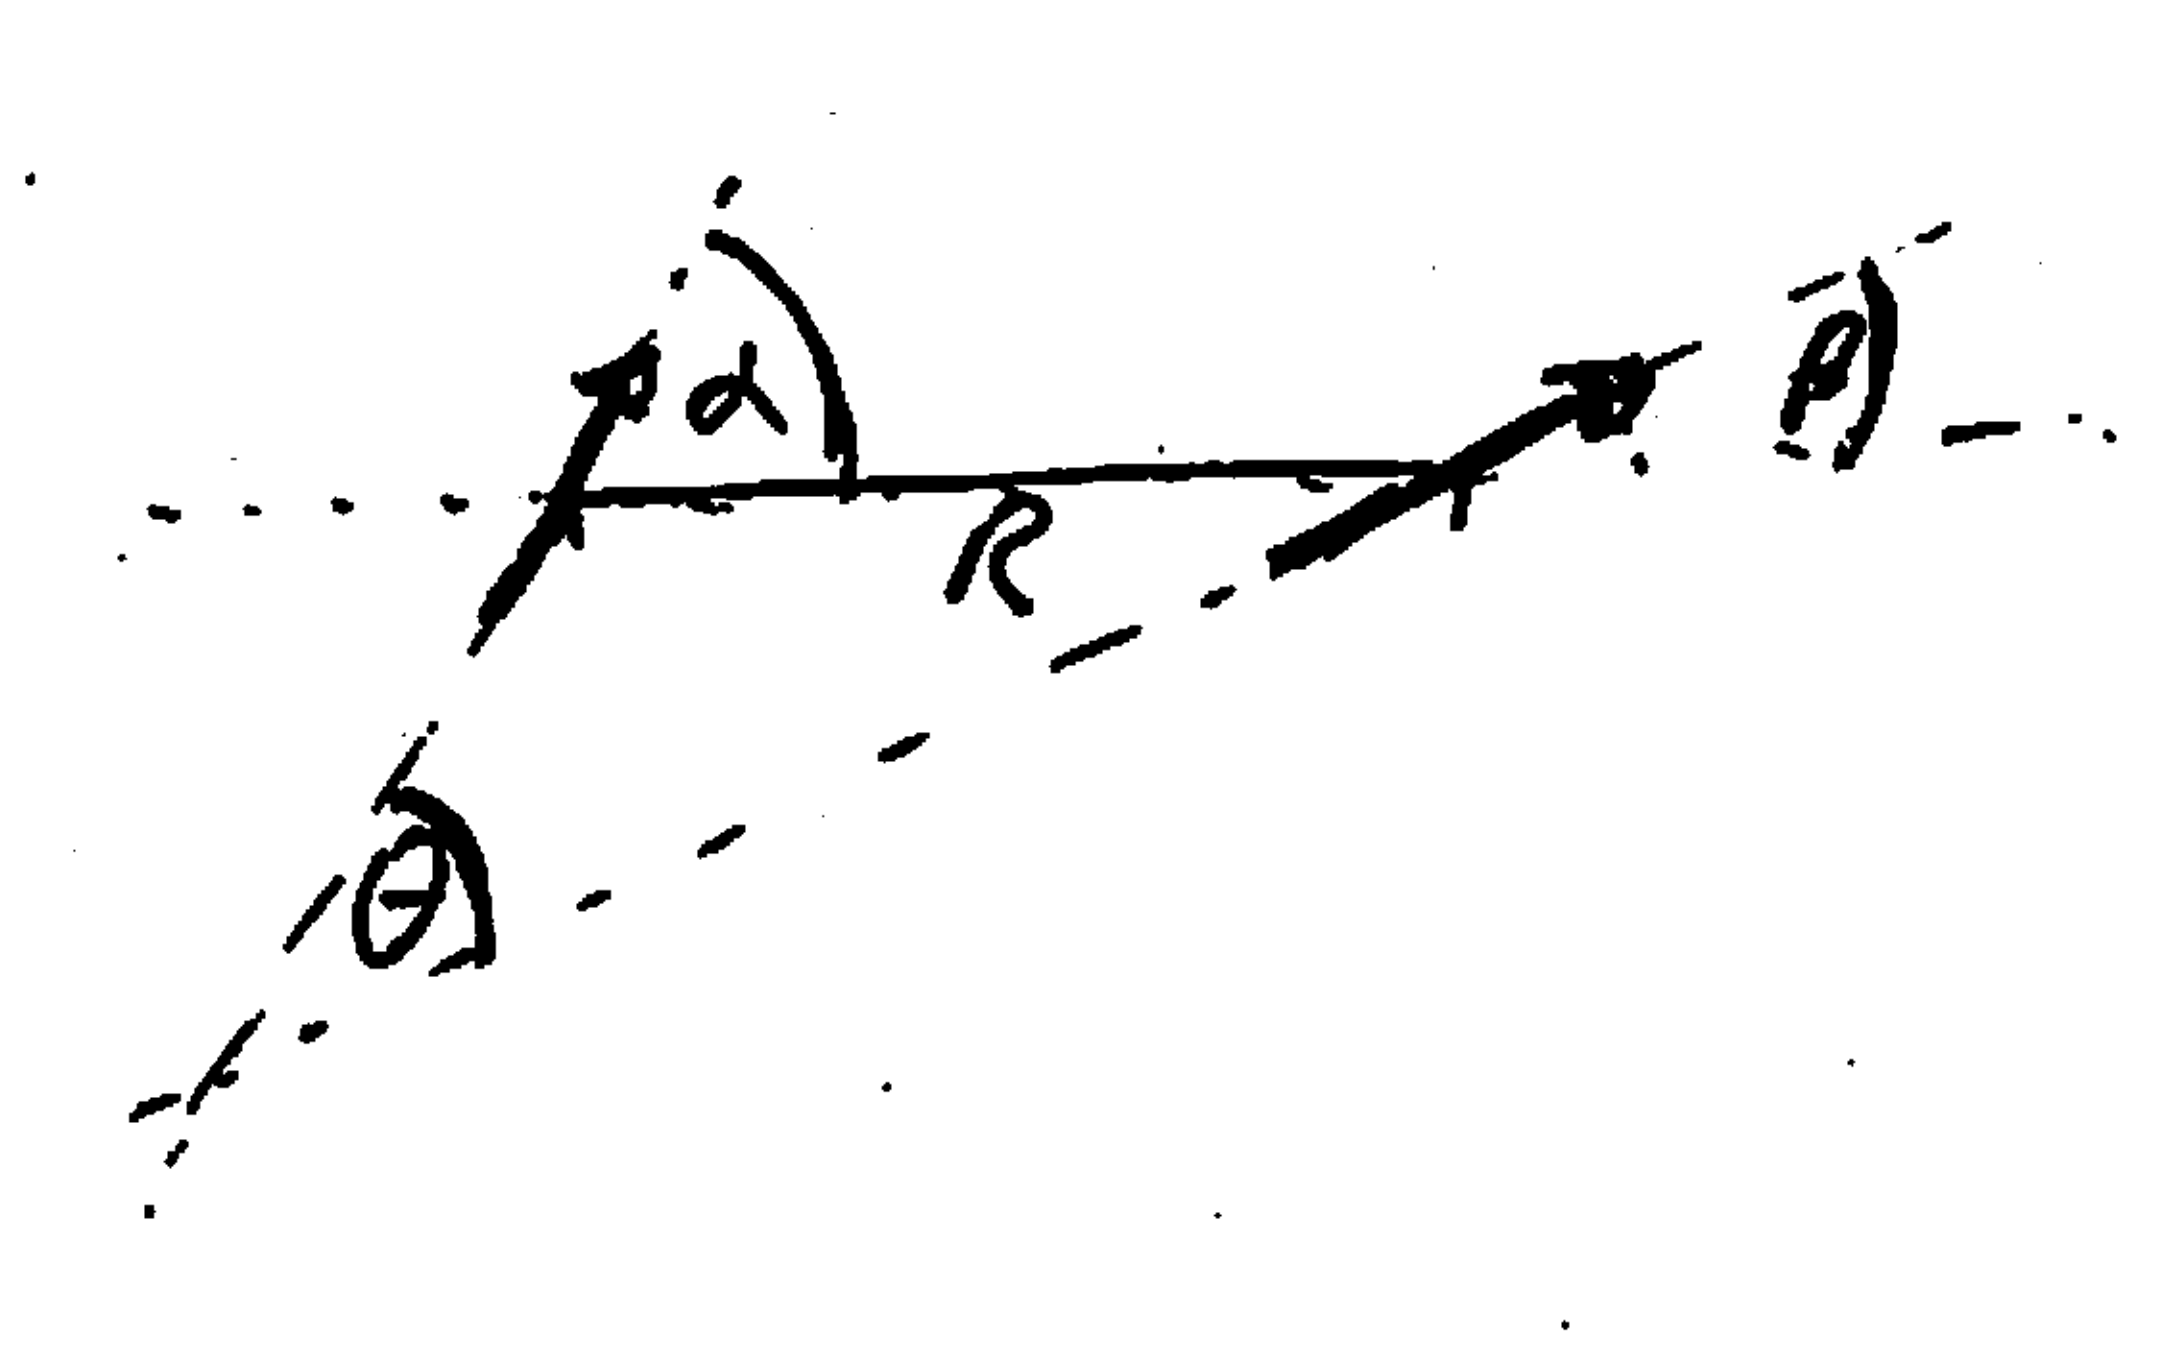
\includegraphics[width=\textwidth]{\currfiledir/angles.png}
   \inputtikz{\currfiledir/angles}

\caption{Sketch showing 
the angles used to calculate the coupling factor $\kappa$}
\end{marginfigure}

A similar coupling term also exist for the non-resonant coupling\footcite{knoester-book}
\begin{equation}
\hat{H}_{non-res} = J \left(  \ket{11}\bra{00} + \ket{00}\bra{11}  \right)
\end{equation}
but this can be ignored, as it is non-resonant. Altogether, the Hamilton operator reads in matrix form
\begin{equation}
\hat{H} = \begin{pmatrix}
0   					& \mu_a 						&	\mu_b						& 		J 		\\
\mu_a^\star	& \hbar \omega_a		&	J								& \mu_b	\\
\mu_b^\star  &  J^\star					& \hbar \omega_b		& \mu_a	\\
J^\star				& \mu_b^\star			& \mu_a^\star			& \hbar (\omega_a + \omega_b) \\
\end{pmatrix} \quad .
\end{equation}
When we ignore the double-excited state $\bra{11}$, the essence in contained in the center $2 \times 2$ matrix which we discussed already in the preceding section.

When $\ket{\psi}$ is a linear combination of $\ket{01}$ and $\ket{10}$, then also the transition dipole moment from $\ket{00}$ to $\ket{\psi}$ is a linear combination of $\mu_a$ and $\mu_b$ with the same weights. When $J \gg |E_a - E_b| / 2$ then we get
\begin{equation}
 \boldsymbol{\mu}_{\pm} = \sqrt{1/2} \, \left( \boldsymbol{\mu}_a \pm  \boldsymbol{\mu}_b  \right)  \quad .
\end{equation}
The brightness of the absorption line is for identical molecules, i.e. $\mu = \mu_a = \mu_b$
\begin{equation}
 I \propto |\boldsymbol{\mu}_{\pm}|^2 = (1/2) \, \left| \boldsymbol{\mu}_a \pm  \boldsymbol{\mu}_b  \right|^2 =  \left( 1 \pm \cos \theta \right) \, \left| \boldsymbol{\mu}   \right| ^2  \quad ,
\end{equation}
where $\theta$ is as above the angle between the transition dipole moments. The same relation hold for the radiative rate.

The spectroscopic signature of coherent coupling between two molecules is thus a splitting of the absorption line into two lines, separated by twice the coupling energy $J$. The sum of the line amplitudes remains unchanged, but in some cases (H- and J-aggregates, see below) one transition will take the whole amplitude and the other remains dark. In these cases, no splitting but a shift of the absorption line is observed. The coupling vanishes when both dipoles are oriented perpendicular to each other ($\theta = 90^\circ$)


\section{H- and J-aggregates}

\begin{marginfigure}
%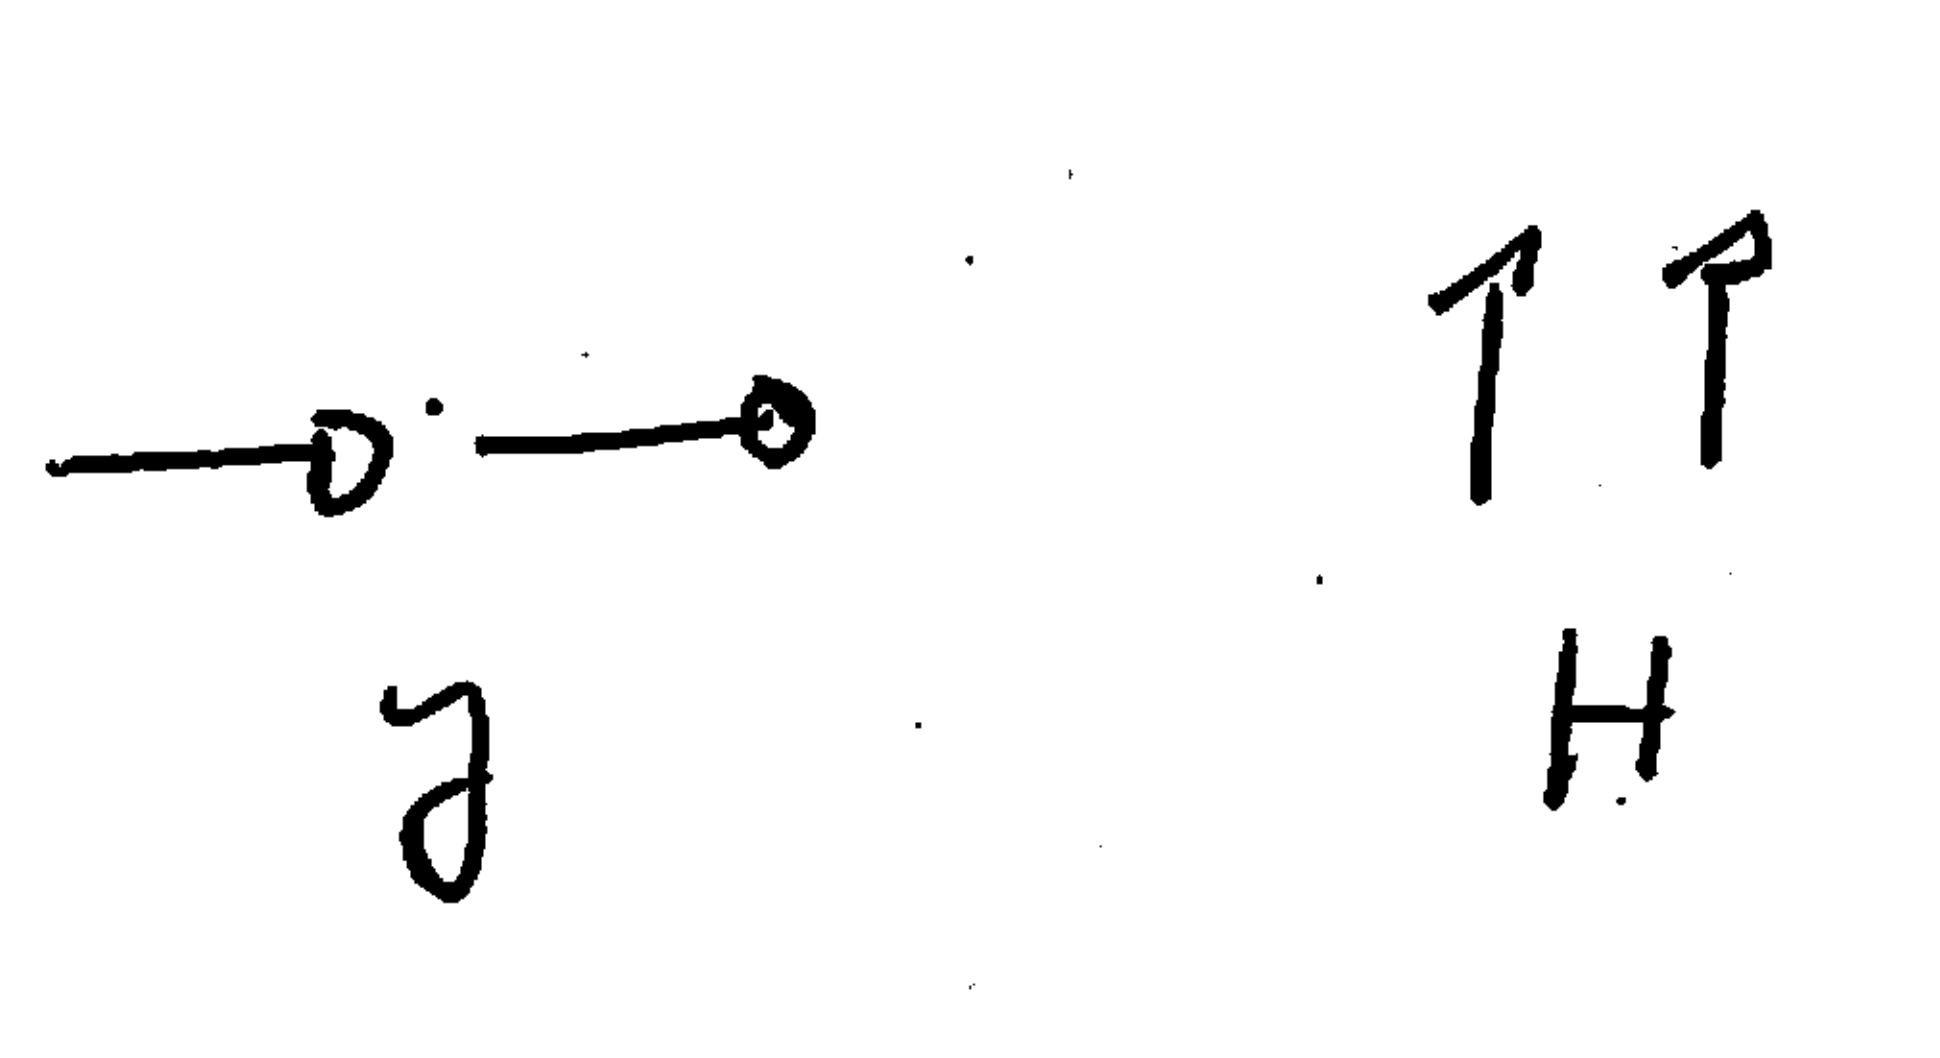
\includegraphics[width=\textwidth]{\currfiledir/aggregates.png}
   \inputtikz{\currfiledir/jh}

\caption{J- and H aggregates.}
\end{marginfigure}


Two important limiting cases are the H- and J-aggregates\footcite[chapters 2.1.4.3, 2.2.5.3]{KoehlerBaessler2015} In a J-aggregate, the dipoles are oriented parallel and head-to-tail, i.e. $\alpha = \beta = \theta = 0$ and therefore $\kappa = -2$. A negative $\kappa$ implies that the coupling constant $J$ is negative. The state $\Psi_+$, which carries all the oscillator strength, has the energy $E_+ = (E_a + E_b) / 2 + J$, which is lower than the average energy of the uncoupled states. The absorption line thus shifts to the red. The same hold for the fluorescence emission spectrum.

In an H-aggregate, the dipoles orient also parallel, but side-to-side, i.e.  $\alpha = \beta = 90^\circ$ and $\theta = 0$. In this case is $\kappa =1$ and $J$ positive. The absorption line shifts to the blue upon formation of aggregates, as again the  $\Psi_+$ state gets all the oscillator strength. However, as fluorescence emission is slow compared to other relaxation processes, this high energy state does not emit light. In emission, H-aggregates appear dark.

The width of the absorption line of a dye at room temperature is determined by dephasing, i.e., fluctuations in the environment that are fast compared to the lifetime of the excited state, and by static differences in the environment of different chromophores. The spectral position of the absorption line in a molecular aggregate is the average of two single chromophore transitions. As in the propagation of uncertainties in an experiment, the width of the new distribution, generated as the average over two values from the old distribution, is reduced by a factor of $\sqrt{2}$. This holds more generally\footcite{Knapp1984}, so that an aggregate of $N$ chromophores is expected to have a spectral line width reduced\sidenote{This is the same physics as motional narrowing in NMR.} by $\sqrt{N}$.




%\begin{tabular}{llll}
%$\theta$	&	$0^\circ$ & $90^\circ$ & $0^\circ$  \\
%$\alpha$ & $0^\circ$ & $0^\circ$ & $90^\circ$  \\
%$\beta$ & $0^\circ$ & $90^\circ$ & $90^\circ$  \\
%$\kappa$  & $-2	$	& 	 $	0	$				& $1$   \\
%\end{tabular}




\printbibliography[segment=\therefsegment,heading=subbibliography]

%
%%%

\chapter{Raman Scattering}

\textit{Ordnen sie die Linien zu und bestimmen sie so die Polymere
}
\section{Experiment}

The data sets contain absorption spectra as measured with a commercial UV/VIS spectrometer. Determine the absorption cross section of each species and compare to its geometrical size. Determine also the oscillator strength, the transition dipole moment, and the transition matrix element.

assuming that almost all atoms are in the ground state ($N_2 \ll N_1$). Note that this absorption cross section $\sigma$ is not a function of angular frequency $\omega$ anymore, but an spectral integrated cross section assuming a black body spectrum.\sidenote{really ???}





\printbibliography[segment=\therefsegment,heading=subbibliography]

%
%%%%-------
%%
%%
\part{Two Level Systems}

\renewcommand{\lastmod}{May 3, 2024}
\renewcommand{\chapterauthors}{Markus Lippitz}


\chapter{Rabi Oscillations}



\section{Tasks}

\begin{itemize}
\item  Visualize the  path of the Bloch vector and its components when a laser pulse shines on a two-level system. Use a numerical method to integrate the differential equation. Investigate both resonant and non-resonant cases.
\end{itemize}



\section{Experiment}

Many experimental realizations show Rabi oscillations. We will discuss them in terms of a two-level system interacting with an optical field, such as an atom in a vacuum or a molecule or quantum dot in a solid state at low temperature. But the same description applies to many other systems. In fact, a two-level system is equivalent to a spin $1/2$ system, such as an electron spin or a nuclear spin. So the same concepts are used in electron spin resonance or nuclear magnetic resonance experiments (ESR and NMR).

We shine a laser beam on an atom, a molecule, a quantum dot. The laser frequency is close to the optical transition. We measure the populations of the excited state, e.g. by fluorescence emission or tunneling of the electron out of this state. We turn on the laser for a given time $t$ and measure the signal amplitude as a function of $t$. This somewhat indirect experiment is necessary because in many cases $t$ is short compared to the emission or tunneling rate. Only in theory can we measure the population of the state as it evolves. We find periodic oscillations of the signal amplitude, the Rabi oscillations.\sidenote{needs papers!}

\section{Density Matrix}


We start by introducing the density matrix.\footcite{Rand2016,Parson,Hamm-dummies}
It is a tool in quantum mechanics to describe not only purely coherent states, but also statistical mixtures, as we will see below. The density matrix is a bit at the edge of the classical canon of quantum mechanics lectures.

When  writing our wave function $\ket{\psi}$ in  a basis $\ket{n}$ as
\begin{equation}
 \ket{\psi} = \sum_n c_n \, \ket{n}
\end{equation}
then we can define a density operator $\hat{\rho}$ as
\begin{equation}
\hat{\rho} =  \ket{\psi}\bra{\psi} = \sum_{m,n} c_n c_m^\star \, \ket{n}\bra{m}
\end{equation}
and the matrix elements of $\hat{\rho}$ are $\rho_{n,m} =  c_n c_m^\star$ or 
\begin{equation}
 \rho = \begin{pmatrix}
  \rho_{00} &   \rho_{01} \\  \rho_{10} &  \rho_{11} \\
 \end{pmatrix} \quad .
\end{equation} 
The density matrix allows to calculate the expectation value of any operator $\hat{A}$ as
\begin{equation}
 \braket{\hat{A}} =  \braket{\psi | \hat{A} | \psi}  = \sum_{m,n} c_n c_m^\star \, A_{m,n} = \sum_{m,n} \rho_{n,m} \,  \, A_{m,n} = Tr ( A \rho) \quad ,
\end{equation}
where the trace sums over the diagonal elements
\begin{equation}
 Tr (U ) = \sum_n U_{n,n}  \quad .
\end{equation}
The trace of the density matrix is one for normalized states 
\begin{equation}
 Tr (\rho) = \sum_n \rho_{n,n} = \sum_n c_n c_n^\star = 1 \quad \text{if normalized} \quad .
\end{equation}
The interesting thing comes when looking at pure and mixed states. Pure states are the 'conventional' states discussed in quantum mechanics, for example this superposition of states
\begin{equation}
\ket{\psi} = \sqrt{\frac{1}{2}} \left( \ket{1} + \ket{2} \right)  \quad .
\end{equation}
In this example, the density matrix reads
\begin{equation}
 \rho = \frac{1}{2} \begin{pmatrix}
 1 & 1 \\ 1 & 1 \\
 \end{pmatrix}
\end{equation}
and its trace is one. But the density matrix also allows to describe new things, beyond pure states, namely statistical mixtures of states. We can describe an ensemble of two-level systems, of which half the ensemble is in state $\ket{1}$, the other half in state $\ket{2}$. This can \emph{not} be written as 
$\ket{1} + \ket{2} $, but a density matrix description is possible. If the statistical probability of each pure state with density matrix $\rho_i$ is $p_i$, then the density matrix of the mixed state is given by
\begin{equation}
\rho_\text{mixed} = \sum_i \, p_i \, \rho_i \quad .
\end{equation}
For a $50:50$ mixture of $\ket{1}$ and  $\ket{2}$ we get
\begin{equation}
 \rho = \frac{1}{2} \begin{pmatrix}
 1 & 0 \\ 0 & 1 \\
 \end{pmatrix} \quad .
\end{equation}
We can distinguish between pure and mixed states by looking at the trace of the squared density matrix
\begin{eqnarray}
 Tr (\rho^2) & = & 1 \quad \text{pure state} \\
 				& < & 1 \quad \text{mixed state.}
\end{eqnarray}

Mixed states can be used not only to describe an ensemble of systems in different states, but also to describe a single system that is in different states at different times. Even if we can do an experiment on a single quantum system, we have to repeat it very often to reduce the noise by averaging. But the experiment does not always follow the same path: either a photon is absorbed or not, but it will most likely not always be absorbed. The time average of such an experiment therefore needs a statistical mixture to describe it.

The diagonal elements of the density matrix describe the populations of the states, i.e. $|c_n|^2$. The off-diagonal elements describe coherence between states. 'Coherence' means 'constant phase relation' or 'possibility to interfere', as with coherent (laser) or incoherent (candle) light. When writing $\ket{1} + \ket{2} $ we have defined the phase between the states to be zero, as  
\begin{equation}
r \, e^{i \phi} = \frac{c_1}{c_2} \quad \text{gives here} \quad \phi = 0 \quad .
\end{equation}
In a statistical mixture there is no\sidenote{better: not enough} coherence between the states, as one sub-ensemble is in one state, another in another state, and they don't know anything of each other.




\begin{questions}

\item For which values of $b$ is the following density matrix describing a pure state ?
\begin{equation*}
 \rho = \frac{1}{2} \, \begin{pmatrix}
1+a & b^\star \\ b & 1-a \\
 \end{pmatrix} 
\end{equation*}
where $a$ is real and $b$ could be complex.

\item Assume a normalized wave function $\ket{\psi} = c_1 \ket{1} + c_2 \ket{2}$. Calculate its density matrix and convince yourself that it describes a pure state.

\item Investigate the off-diagonal elements of a density matrix describing a $50:50$ mixture of $\ket{1}$ and $\sqrt{1/2}(\ket{1} + \ket{2})$. \label{q:rabi_coherence_mixture}


\end{questions}




\section{Liouville--von Neumann equation}

We can construct a differential equation for the time evolution of the density matrix that is a direct analogue of the Schrödinger equation, just that is also takes mixed states into account.

The time-derivative of the density operator $\hat{\rho}$ is
\begin{equation}
 \frac{d}{dt} \hat{\rho}= \frac{d}{dt} \left( \ket{\psi} \bra{\psi} \right) 
 =  \left( \frac{d}{dt}  \ket{\psi} \right) \bra{\psi} 
 + \ket{\psi} \left( \frac{d}{dt}  \bra{\psi} \right)  \quad .
\end{equation}
Making use of the Schrödinger equation
\begin{equation}
 \frac{d}{dt} \ket{\psi} = - \frac{i}{\hbar} \, \hat{H} \, \ket{\psi}
\end{equation}
we get the \emph{Liouville--von Neumann equation}
\begin{equation}
 \frac{d}{dt} \hat{\rho} = - \frac{i}{\hbar} 
 \left[ \hat{H} ,\hat{\rho} \right]  \quad .
\end{equation}

As an example, let us look at a two-level system with the eigen-energies $E_0= 0$ and $E_1 = \hbar \omega_0$. The Hamilton operator is thus
\begin{equation}
 H  = \begin{pmatrix}
  0 & 0 \\ 0 & \hbar \omega_0 \\
 \end{pmatrix} \quad .
\end{equation}
The commutator becomes
\begin{equation}
 \left[ \hat{H}, \hat{\rho}\right] = 
 \begin{pmatrix}
 0 & - \hbar \omega_0 \, \rho_{01} \\   \hbar \omega_0 \, \rho_{10} & 0 \\
 \end{pmatrix} \quad . \label{eq:rabi_density_commutator}
\end{equation}
The  diagonal elements of the density matrix $\rho$, i.e., the populations, remain thus constant in time, as expected for this Hamiltonian. The off-diagonal elements, the coherences acquire a phase-factor proportional to the energy difference, i.e.
\begin{equation}
 \rho_{01}(t) =  \rho_{01}(0) \, \exp \left(i \, \omega_0 \, t \right)  \quad . \label{eq:rabi_coherence_time_evolution}
\end{equation}



\begin{questions}
\item Derive eqs. \ref{eq:rabi_density_commutator} and \ref{eq:rabi_coherence_time_evolution}.
\end{questions}


\section{Optical Bloch Equations}

Now we switch on light and add an interaction Hamiltonian $\hat{H}_I = -\boldsymbol{\mu} \, \boldsymbol{E}$ with the  dipole operator $\boldsymbol{\mu} $ and the optical field   $\boldsymbol{E}$. In total, the Hamilton operator reads\footcite[chap. 3.8]{Rand2016}
\begin{equation}
 \hat{H } = \begin{pmatrix}
  0 & - {\boldsymbol{\mu}} \, \boldsymbol{E} \\ - {\boldsymbol{\mu}}^\star \, \boldsymbol{E}^\star & \hbar \omega_0 \\
 \end{pmatrix} \quad . \label{eq:rabi_bloch_hamiltonian}
\end{equation}
The differential equations for the density matrix become the \emph{Bloch equations}
\begin{eqnarray}
\dot{\rho}_{00} &=&  - \frac{i}{\hbar} \left( \rho_{01} \boldsymbol{\mu}^\star \, \boldsymbol{E}^\star - \rho_{10} \boldsymbol{\mu} \, \boldsymbol{E} \right) 
\label{eq:rabi_bloch_rho00}  \\
%
\dot{\rho}_{11} &=&  - \frac{i}{\hbar} \left( \rho_{10} \boldsymbol{\mu} \, \boldsymbol{E} - \rho_{01} \boldsymbol{\mu}^\star \, \boldsymbol{E}^\star \right) \\
%
\dot{\rho}_{01} &=& - \frac{i}{\hbar}  \left( - \rho_{01} \hbar \omega_0 + (\rho_{00} - \rho_{11})  \boldsymbol{\mu} \, \boldsymbol{E}\right) \\
%
\dot{\rho}_{10} &=& - \frac{i}{\hbar}  \left( + \rho_{10} \hbar \omega_0 + (\rho_{11} - \rho_{00})  \boldsymbol{\mu}^\star \, \boldsymbol{E}^\star \right) 
\label{eq:rabi_bloch_rho10}  %
\end{eqnarray}
These are effectively only 3 differential equations, as the wave function has to stay normalized, i.e., $\rho_{00} +\rho_{11} = 1$.
We can simplify things by skipping some algebraic transformations and introducing the \emph{Bloch vector} $\boldsymbol{S}$ with
\begin{equation}
\boldsymbol{S} = 
\begin{pmatrix}
u \\ v \\ w \\
\end{pmatrix}
= 
\begin{pmatrix}
\rho_{01} + \rho_{10} \\ i (\rho_{01} - \rho_{10}) \\ \rho_{00} - \rho_{11} \\
\end{pmatrix}
= 
\begin{pmatrix}
2 \Re (\rho_{01})  \\ \ 2 \Im (\rho_{01}) \\ \rho_{00} - \rho_{11} \\
\end{pmatrix} \quad .
\end{equation}
The density matrix elements are recovered by
\begin{equation}
 \rho = \frac{1}{2} 
 \begin{pmatrix}
 1+ w & u - i v \\ u + i v & 1 - w\\
 \end{pmatrix}
\end{equation}
With this we can write the system of differential equation as 
\begin{equation}
 \dot{\boldsymbol{S}} = \boldsymbol{M}   \times \boldsymbol{S} 
 \quad \text{with} \quad 
 \boldsymbol{M}  = 
 \begin{pmatrix}
 -\frac{2}{\hbar} \, \Re ( \boldsymbol{\mu} \, \boldsymbol{E} ) \\
 - \frac{2}{\hbar} \, \Im ( \boldsymbol{\mu} \, \boldsymbol{E} ) \\
  \omega_0
 \end{pmatrix} \quad .
\end{equation}
The time evolution of the Bloch vector, and by this of the density matrix, can be described by the action of a torque vector $\boldsymbol{M}$. 


These equations were derived by Felix Bloch for the magnetization of an ensemble of atomic nuclei in an NMR experiment. For nuclear or electronic (ESR) magnetic moments, the vector corresponds to the direction of the ensemble average of the magnetization, i.e. it is a real-space vector in the laboratory frame. In our case, $\mathbf{S}$ is a vector in an abstract 3d vector space describing the density matrix of an ensemble of two-level systems. So I use $uvw$ instead of $xyz$, but the physics is the same. Also spin-1/2 systems like electron spins or nuclear spins in ESR and NMR experiments form a two-level system.


Without optical field, the Bloch vector rotates around its $w$ axis, as seen in the phase oscillation of the coherences in the last section. With optical field, also the populations changes, and things become complicated.
To simplify things, we assume that our optical field is a single mode with a slowly varying amplitude only, i.e.
\begin{equation}
 \boldsymbol{E}(t) = \boldsymbol{x} \, E_0(t) \left( e^{i \omega_L t} + e^{-i \omega_L t} \right) \quad .
\end{equation}
The time-dependence of $E_0(t)$ should be slow compared to $\omega_L$. This is the slowly varying amplitude approximation (SVEA). We do the same with the off-diagonal elements of the density matrix
\begin{equation}
 \rho_{01}' = \rho_{01} \, e^{-i \omega_L t}  \quad \text{and} \quad
 \rho_{10}' = \rho_{10} \, e^{+i \omega_L t} = \rho_{01}'^\star \quad .
\end{equation}
We thus factor out a phase oscillation with the laser frequency and keep only the slowly varying rest.\sidenote{The diagonal elements do not phase-rotate and remain unchanged.} Inspecting the differential equations for the density matrix, this leads together with our definition of $\boldsymbol{E}$ to the following modifications
\begin{equation}
 \omega_0 \rightarrow \omega_0 - \omega_L \quad \text{and} \quad 
 \boldsymbol{\mu} \, \boldsymbol{E}  \rightarrow \mu \, E_0  \, ( 1+ e^{i 2\omega_L t} ) \approx \mu \, E_0  \quad .
\end{equation}
As we assumed the elements of $\rho'$ to vary slowly, we neglect the term $\exp(i 2 \omega_L t)$, as it will average out.  This is the rotating wave approximation (RWA). Effectively, we are going into a 
rotating frame. Our new coordinate system rotates around the $w$ axis with the angular frequency of the laser $\omega_L$. The optical frequency of the transition $\omega_0$ is close to this laser frequency. We neglect terms of $\omega_0 + \omega_L$ and only keep terms of  $\omega_0 - \omega_L$. In total we get\sidenote{someone should check this!}
\begin{equation}
 \dot{\boldsymbol{S}'} = \boldsymbol{M}'   \times \boldsymbol{S}' 
 \quad \text{with} \quad 
 \boldsymbol{M}'  = 
 \begin{pmatrix}
- \mu    E_0(t) / \hbar \\
0 \\
\omega_0 - \omega_L
 \end{pmatrix} = 
  \begin{pmatrix}
- \Omega \\
0 \\
\omega_0 - \omega_L
 \end{pmatrix}  \label{eq:rabi_bloch_vector_RWA}
\end{equation}
with the (angular) Rabi frequency\sidenote{Some definitions include a factor of 2 here.} $\hbar \Omega = \mu    E_0(t) $ and $\mu = \boldsymbol{\mu \, x}$ the projection of the transition dipole moment on the polarization direction of the light field. In the following, we stay in the rotating frame and leave out the prime symbols.



\begin{questions}

\item Derive the Bloch  equations \ref{eq:rabi_bloch_rho00}  to \ref{eq:rabi_bloch_rho10}  
from the Hamilton operator eq. \ref{eq:rabi_bloch_hamiltonian} and the Liouville-von Neumann equation.

\end{questions}

\section{Rabi Oscillations}

Let us discuss the time evolution of the Bloch vector in the rotating frame. Applying only a torque $\boldsymbol{M}$, the length of the Bloch vector does not change. It moves along the surface of a sphere, the \emph{Bloch sphere}. The sphere has a diameter of one when the density matrix describes a normalized pure state. For mixed states, the Bloch vector is shorter. Below we will see how dephasing and relaxation processes reduce the length of the Bloch vector.


A two-level system in the ground state is on the north pole of the sphere. The state $\ket{0} + \ket{1}$ is on the equator, pointing along the $u$ axis. All points except the poles contain a coherence between the two levels.


\begin{marginfigure}
\centering
\input{\currfiledir blochsphere.tikz.tex}
\caption{Some Bloch vectors and their positions on the Bloch sphere. \label{fig:rabi_bloch_sphere}}
\end{marginfigure}


The torque $\boldsymbol{M}$ rotates the Bloch vector around  $\boldsymbol{M}$ with a angular frequency  $|\boldsymbol{M}|$. A resonant laser field, i.e., $\omega_L = \omega_0$ rotates the Bloch vector around the $u$ axis. When this field acts continuously, the Bloch vector moves from the north pole via the equator to the south pole and back to the north pole and so on. The population of the state changes periodically from zero to one:
\begin{equation}
 \rho_{00} = \cos ( \Omega \, t / 2)^2 \quad .
\end{equation}
These are the \emph{Rabi oscillations}. In a laser pulse, the amplitude $E_0(t)$ of the optical field varies, for example like a Gaussian. In this case, the instantaneous Rabi frequency $\Omega$ also varies and it is convenient to quantify the total effect of a single pulse by the \emph{pulse area $\theta$}
\begin{equation}
 \theta = \int_{pulse} \Omega (t) \, dt \quad .
\end{equation}
A $\pi$ pulse, acting on a system in the ground state, will thus lead to a system in the excited state. A $2\pi$ pulse leaves the populations unchanged.\sidenote{but has an effect on the phase}


When the laser is not fully resonant, the Bloch vector is rotated around an axis in the $u$-$w$ plane. Starting from the ground state at the north pole, it thus does not reach the south pole anymore. The population of the excited state will  not reach one. At the same time, the phase oscillations of the two-level system are not fully taken care of by the rotating frame anymore. A little bit of rotation remains. In combination, this gives a complicated precession of the Bloch vector $S$ around the torque $M$ with an effective Rabi frequency 
\begin{equation}
 \Omega_\text{eff} = \sqrt{\Omega^2 + (\omega_0 - \omega_L)^2 } \quad .
\end{equation}

\begin{marginfigure} 
  \inputtikz{\currfiledir rabiosc}
    \caption{Rabi oscillations}
    \label{fig:Rabi}
\end{marginfigure}

We can observe these oscillations by any method that can determine the population of the excited state, for example fluorescence emission, electron emission or (transient) absorption.



\begin{questions}

\item Re-visit questions 1--3 from above and discuss the density matrix on the Bloch sphere.

\item Write a computer program to calculate the trajectory of the Bloch vector in the rotating wave approximation, eq. \ref{eq:rabi_bloch_vector_RWA}. Use
\begin{equation*}
 \boldsymbol{S}'(t + \Delta t) \approx  \boldsymbol{S}'(t ) + \Delta t \,  \boldsymbol{M}'   \times \boldsymbol{S}' (t)
\end{equation*}
with a small enough $\Delta t$. The approximation holds when $|\boldsymbol{S}' (t)| $ remains close to one. Plot $\boldsymbol{S}' (t)$ in 3D on the Bloch sphere (Fig.\ref{fig:rabi_bloch_sphere}) and in 2D as function of time.

\end{questions}

\section{Damping and dephasing}

In reality, both a coherence as well as the population of an excited state decays in the course of time. Without going into further detail, we can add these processes phenomenologically as Lindblad operator $\boldsymbol{L}$ to the Liouville-von Neumann equation
\begin{equation}
    i\hbar \dot{\hat{\rho}} =
    [\hat{H},\hat{\rho}] - \boldsymbol{L}  \hat{\rho} \quad .
\end{equation}
Excited state populations decay exponentially with a lifetime $T_1$. The coherence between two states decays with a time constant $T_2$ with
\begin{equation}
    \frac{1}{T_2} = \frac{1}{T_2^\star} + \frac{1}{2 \, T_1} \quad ,
\end{equation}
where $T_2^\star$ is called pure dephasing time. The $T_1$ time enters, as a decaying population also removes coherence. The prefactor of $2$ is a consequence of effective spin-$1/2$-system. On the Bloch sphere, these processes let the Bloch vector move back to the north pole, but not along the surface of the sphere but with varying length of the vector.\sidenote{In the original work of Bloch this scheme was applied to the magnetization of a spin-$1/2$ system which decays towards the center of the sphere, as thermal energy leads to almost equal population of both states.}



\printbibliography[segment=\therefsegment,heading=subbibliography]

\renewcommand{\lastmod}{Mai 29, 2024}
\renewcommand{\chapterauthors}{Markus Lippitz}


\chapter{(Perturbed) Free Induction Decay}
\label{chap:fid}


\section{Tasks}

\begin{itemize}
\item Reproduce Fig. 4b of \cite{Wolpert:2012hs} to model the data in Fig. 4a. As the quantum dot is buried beneath the surface, the reflected reference field $E_0$ is in its phase earlier than the signal field $E_S$ of the dot. In this sample, the lag is $\Delta \phi = 0.4 \pi$. See also question \ref{qe:7_fid_sim} below.
\end{itemize}

\begin{figure}
\centering
\includegraphics[width=0.8\textwidth]{\currfiledir figure_rho.pdf}
\caption{Perturbed free induction decay (at negative delay $\tau$) of a single GaAs quantum dot measured by pump-probe spectroscopy \citep{Wolpert:2012hs}. At negative delay, the pump comes after the probe pulse.} \label{fig:fid_wolpert}
\end{figure}

\section{Experiment}

In the experiment, one measures the change in the spectrum of a probe pulse due to the presence of a pump pulse. The probe pulse is reflected at a sample surface under which a quantum dot is buried. The vertical slices of the figure contain the spectrum. The energy axis is relative to the quantum dot transition energy. The pulse is temporally short ($\approx 1 $ps) and thus spectrally broad. The pump pulse is also short, and comes at a variable delay before or after the probe pulse (positive delay means pump before probe). The pump pulse is switched on and off, and the figure contains only the difference in reflected probe spectrum (grey means no difference). As only the quantum dot is influenced by the pump pulse, this makes visible the small contribution of the quantum dot reflectivity.
At positive pump-probe delays, the pump comes before the probe and the spectrum is just the expected absorption spectrum. At negative delays, the probe comes before the pump pulse, and the spectrum shows fringes that increase in spacing with decreasing pump-probe delay. This is the perturbed free induction decay. The diagonal element of the density matrix is created by the probe pulse and removed by the pump. In between, it radiates a field that we see in the spectrum.

\begin{marginfigure}
\inputtikz{\currfiledir v-system}
\caption{Sketch of a V-level system. The energy difference is the fine structure splitting (FSS).}
\end{marginfigure}


To understand the influence of the pump pulse, we need to look more in detail at the levels of an epitaxial  quantum dot, which can  can be approximated by a V-shaped level system: depending on the polarization direction of the light, two different excited states $\ket{h}$ and $\ket{v}$
 can be populated. The excited states differ in the spin of the electron, so that an interchange is slow on the relevant timescales. Such a V-system allows to use one transition as 'normal' two-level system, and the other transition to switch off the first: when the system is in $\ket{v}$, the transition $\braket{h | \mu | g}$ is not possible anymore. This does not change much the physics, but makes experiments much simpler, as the influence of the  $\braket{h | \mu | g}$ transition can be modulated in a pump-probe scheme and is such much easier to detect.
 


\section{Pump-Probe Experiments}

The timescale of the experiment is set by the decay of the coherence and the populations. In many cases, this is faster than the temporal resolution of photodetectors. One method to investigate the dynamics of a system under these conditions is pump-probe spectroscopy. A pump-pulse starts a process and some (short) time later, a probe-pulse interrogates the system. The detector does not need a time resolution and can average over many pump-probe pulse pairs. The time resolution comes by the pulse length and their temporal separation. In many cases, the effect of the pump pulse on the system is weak, i.e. the probe pulse would measure almost the same, independent whether the pump was present or not. To increase the signal to noise ratio in these cases, on investigates the relative change of the signal
\begin{equation}
 \frac{\Delta I}{I} = \frac{I_\text{with pump} - I_\text{without pump} }{I_\text{without pump}} \quad .
\end{equation}
The pump-pulse is switched using a mechanical chopper or an acousto-optical modulator at as high as possible frequencies to avoid $1/f$-noise. The detector should only detect the probe pulse (and the field radiated by the coherence), otherwise $\Delta I$ is overwhelmed by leaking pump pulse. A convenient way to discriminate pump and probe is the polarization direction of the light field, setting the orientation of the transition dipole moment at $45^\circ$ between pump and probe.

\begin{questions}

\item Estimate the fraction of probe power that is absorbed by the quantum dot, i.e., that is then missing in the reflected beam. The numerical aperture of the microscope objective is about 0.5. The spectral width of a pixel of the CCD camera is about 100 \textmu eV.

\end{questions}
 

\section{Coherence as a Source of Radiation}


Let us look at methods to measure elements of the density matrix $\rho$. We can measure populations, i.e., diagonal elements of $\rho$ by fluorescence emission or electron tunneling. If an atom, molecule, quantum dot is in the excited state, it can emit a fluorescence photon and revert to the ground state. All coherence is lost in this process, neither the fluorescence photon nor the ground state carries any phase relation to the excited state. The excited state is also destroyed, as afterwards the system is in the ground state. But we can observe the fluorescence photon and from the fluorescence rate we can determine how many systems of an ensemble or how often a single system is (better: was) in the excited state. We thus measure population of the emitting state. In the same way, we can use electrons tunneling out of the excited state, for example in a diode structure which also supplies  a new electron to the ground state. Also this tunneling signal is incoherent.

We can also measure coherences, i.e., off-diagonal elements in the density matrix $\rho$, as these coherences are the source of radiation. To see this, we need to connect the microscopic description by the density matrix to the macroscopic world of Maxwell's equations, resulting in the Maxwell-Bloch equations \footcite[chapter 8.3]{MilonniEberly1988} \footcite[chapter 3.9]{Rand2016}\footcite{Meschede-OLL}. This is what the expectation value does. The  polarization $p$ of a single two-level system at position $z$ in the  laser beam is given by the expectation value of the polarization operator $\hat{\mu}$
\begin{equation}
 p(t,z) = \braket{\hat{\mu}} = Tr ( \mu \, \rho) = \mu_{01} \rho_{10}'  \, e^{-i (\omega_L t - k z)}  \quad ,
\end{equation}
where the polarization operator has only off-diagonal entries in the matrix representation.\sidenote{Only the real part has physical significance, or, we leave out the complex-conjugate part here.} The prime signals denote once more the density matrix in the rotating frame. The macroscopic polarization $P = N \, p$ of a volume of identical atoms is a source term in the one-dimensional wave equation
\begin{equation}
  \frac{\partial^2}{\partial z^2} \boldsymbol{E}_S  - \frac{1}{c^2} \frac{\partial^2}{\partial t^2} \boldsymbol{E}_S 
 =  
\frac{1}{c^2\, \epsilon_0} \frac{\partial^2}{\partial t^2} \boldsymbol{P}   \quad .
\end{equation}
$ \boldsymbol{E}_S$ is the  generated field:
\begin{equation}
 \boldsymbol{E}_S =   E_S(z,t) \, e^{-i (\omega_L t - k z)}   \quad . \label{eq:fid_def_ES}
\end{equation}
We assume that its amplitude $E_S(z,t) $ varies slowly in time and space, i.e., we use the  slowly-varying envelope approximation and get (with $\rho_{10}' = u - i v$)
\begin{equation}
  \frac{\partial}{\partial z} E_S  - \frac{1}{c} \frac{\partial}{\partial t} E_S
 =  
N \frac{i k }{2 \epsilon_0}  \mu_{01} ( u - i v) \quad .
\end{equation}
This forms together with the Bloch equations from last chapter the Maxwell-Bloch equations of a coupled light-matter system. As solution we find
\begin{equation}
 E_S = N L \frac{i k }{2 \epsilon_0}  \mu_{01} ( u - i v)
 =
  N L \frac{k }{2 \epsilon_0}  \mu_{01} (v + i u)
  \propto \mu_{01} \Im (\rho_{01}' )  \quad .
\end{equation}
It is thus the $v$ component of the Bloch vector (or $\Im (\rho_{01}'$) ) that produces the optical field\footcite[chapter V.B.1]{CT-atom-photon}.
%
%The resulting field is\footcite[eq. 4.4]{Hamm-dummies}\footcite[eq. 3.9.16 !! update nomenclature !!]{Rand2016}
%\begin{equation}
%  E_{out} \propto -i \, P \propto - \mu_{01} \, \Im ( \rho_{01} )
%\end{equation}


\begin{questions}

\item Read in a  textbook of your choice on the wave equation with a source term. Usually this is discussed in 3d for dipole radiation and in 1d for lasers.

\item Which requirements on  $E_S(z,t) $ does the slowly-varying envelope approximation have to transform second to first order derivatives along space and time?

\item Think about Fermi's Golden Rule (chapter 1) and how the transition matrix element $\braket{2|\hat{\mu}|1}$ is necessary for absorption. Compare the temporal evolution of $\braket{2|\hat{\mathbf{r}}|1}$ with that of a system at the equator of the Bloch sphere.
\end{questions}



\section{Absorption of a single photon}

\begin{marginfigure}
\hspace*{\fill} \input{\currfiledir blochsphere_pi.tikz.tex}
\caption{A $\pi$ pulse acting on the ground state.}
\end{marginfigure}


Let us discuss as example the absorption of a single photon, which transfers the system from the ground state to the excited state, or equivalently is the action of a $\pi$-pulse. We start by a two-level system in the ground state. The Bloch vector points to the north pole. We shine in an optical field on resonance with the system ($\omega_0 = \omega_L$). The duration of the light pulse $\Delta t$ should be such that is a $\pi$-pulse, i.e.
\begin{equation}
 \theta = \pi = \int_0^{\Delta t} \, \Omega(t) \, dt =  \int_0^{\Delta t} \, \frac{ \mu \, E(t)}{\hbar} \, dt \quad .
\end{equation}
When the light pulse has the amplitude $E_0$ during $t= 0 \cdots \Delta t$ we get
\begin{equation}
 \Delta t = \pi \frac{\hbar}{\mu E_0}  = \pi \, \frac{1}{\Omega} \quad .
\end{equation} 
The $w$ component of the Bloch vector follows the Rabi oscillation, i.e.
\begin{equation}
 w(t) = \cos ( \Omega t  ) = \cos \left( \pi  \frac{t}{\Delta t} \right) 
\end{equation}
and the excited state population accordingly
\begin{equation}
 \rho'_{11}(t) = \frac{1 - w}{2}  = \sin^2 ( \Omega t /2 ) \quad .
\end{equation}
%
\begin{marginfigure}[-49mm]
\inputtikz{\currfiledir rho_photon}
\caption{Absorption of a photon as seen in the density matrix}
\label{fig:fid_rho_single_photon}
\end{marginfigure}
%
The imaginary part of the coherence, related to the $v$ component of the Bloch vector, is
\begin{equation}
 \Im (\rho'_{01} ) = \frac{1}{2} v =  - \frac{1}{2}  \sin \left( \pi \frac{t}{\Delta t} \right) \quad .
\end{equation}
The radiated field is 
\begin{equation}
 E_S  = N L \frac{k }{\epsilon_0}  \mu_{01} \Im (\rho_{01}' ) 
 = - N L \frac{k }{2 \epsilon_0}  \mu_{01} \sin \left( \pi \frac{t}{\Delta t} \right) \quad .
\end{equation}
On the detector, the pumping field $E_0$ and the radiated field $E_S$ interfere. We measure the power $P$ of a single pulse per area of the beam  
\begin{equation}
P  = \frac{1}{2} \epsilon_0 c \, \int_\text{pulse} | E_0 + E_S |^2 \ dt \quad .\label{eq:fid_P}
\end{equation}
The presence of the absorbing two-level system leads to a change in detected power density, assuming real-valued amplitudes with $E_S \ll E_0$
\begin{equation}
 \Delta P = \frac{1}{2} \epsilon_0 c \,  
\int_\text{pulse} 2 E_0 E_S  \ dt
  =-   \sigma \frac{k c }{2}  E_0 \mu_{01}  \int_0^{\Delta t}   \sin \left( \pi \frac{t}{\Delta t} \right)  \,  dt  \label{eq:fid_delta_P}
\end{equation}
where $\sigma = N L $ is the projected area density of the two-level systems. The integral gives $2 \Delta t/\pi$ so that
\begin{equation}
 \Delta P =-  \sigma \frac{k c}{2}  E_0 \mu_{01} \frac{2 \Delta t}{\pi}
= -  \sigma k c   E_0 \mu_{01}  \frac{\hbar}{\mu E_0} 
= -  \sigma \,  \hbar \omega   \quad .
\end{equation}
Each atom removes the energy of one photon!


\begin{questions}
\item Using your code to integrate the Bloch equations from last chapter, reproduce fig. \ref{fig:fid_rho_single_photon}. Calculate $\Delta P$  with eqs. \ref{eq:fid_P} and \ref{eq:fid_delta_P} for arbitrary detuning between laser and quantum dot and for arbitrary pulse length. Plot an absorption spectrum by scanning the laser frequency. What determines the spectral width?
\end{questions}



\section{Absorption of half of a photon}

\begin{marginfigure}
\input{\currfiledir blochsphere_pi_half.tikz.tex}
\caption{A  $\pi/2$ pulse acting on the ground state.}
\end{marginfigure}

We keep the amplitude of the laser field the same but reduce the pulse length to $\Delta t / 2$, i.e. a $\pi/2$ pulse. This does only change the upper limit in the integral, so that 
\begin{equation}
 \Delta P 
= -  \frac{1}{2} \sigma \,  \hbar \omega   \quad .
\end{equation}
Each atom removes half the energy  of a photon. How is that possible?  Here the power of the density matrix comes into play. It describes a statistical ensemble. Half of the atoms absorb a photon, half of them don't. But all atoms undergo the $\pi/2$ Rabi cycle, moving the Bloch vector into the equatorial plane, and describing a state $\ket{\psi}$
\begin{equation}
 \ket{\psi} = \sqrt{\frac{1}{2}} \left( \ket{0} - i \, \ket{1} \right) \quad .
\end{equation}
However, at this point our experiment is not finished yet. We still have coherence in the system, it is not decided yet if  Schrödinger's cat is dead or alive. The experiment is finished only when all coherence has decayed, into
\begin{equation}
 \ket{\psi} = \ket{0}  \quad \text{or} \quad \ket{\psi} = \ket{1}  \quad .
\end{equation}
When the decay of  coherence is much faster than population decay,  both final states will be reached with equal probability. On average, each atom absorbs half the energy of a photon.


\section{Spectra}

Even after applying the slowly-varying envelop approximation, the amplitude $E(t)$ of the electric field is varying so fast that we can not measure it. Even the fastest photo detectors have a response time of only picoseconds. We can measure time-integrated properties, such as $P$ in eq. \ref{eq:fid_P}. Or we can measure properties related to the Fourier transform of  $E(t)$. This is what a spectrometer does. Diffraction at the grating performs the Fourier transform. The CCD chip then measures
\begin{equation}
 P (\omega) d\omega =  \frac{1}{2} \epsilon_0 c \,  \left| E(\omega) \right|^2 \ d\omega =  \frac{1}{2} \epsilon_0 c \,  \left|  \mathcal{FT} ( E(t) ) \right|^2 \ d\omega
\end{equation}
When interpreting the frequency $\omega$ in this equation, we have to pay attention to the definition of $E(t) $. If it contains a part $e^{i \omega_0 t}$ oscillating with the frequency of the optical field, then also $\omega$ is an optical frequency of some 100~THz. If the carrier frequency is split off, as in eq.  \ref{eq:fid_def_ES}, the frequency of the Fourier transform is only additive to the carrier frequency, can thus be much lower than THz. This comes from the convolution property of Fourier transforms
\begin{align}
 \mathcal{FT} \left( E(t) \, e^{i \omega_0 t} \right) 
  = &
  \mathcal{FT} \left( E(t)  \right)  \otimes
 \mathcal{FT} \left(  e^{i \omega_0 t} \right)  \\
 = &
  E(\omega) \otimes
\delta (\omega - \omega_0 ) =  
E (\omega - \omega_0 )
\end{align}
where $\otimes$ is the convolution operator. 

We  Fourier transform the fields with and without pump pulse 
and subtract the resulting intensities. Using $E_S \ll E_0$ we get
\begin{equation}
 \left| E_0(\omega) + E_S(\omega) \right|^2 -  \left| E_0(\omega)  \right|^2 \approx 2  \Re \left[ E_0(\omega)^\star   \, E_S(\omega)  \right] \label{eq:fid_delta_E_spec}
\end{equation}
or
\begin{equation}
\Delta P (\omega) =  \epsilon_0 c \, \, \Re \left[  E_0(\omega)^\star   \, E_S(\omega)  \right] \label{eq:fid_delta_P_spec}
\end{equation}


\begin{questions}

\item Derive  eqs. \ref{eq:fid_delta_E_spec} and\ref{eq:fid_delta_P_spec}.% (and check if there is a factor $2$ missing).

\end{questions}
 

\section{Free induction decay}

We discussed how a coherence in a two-level system is generated, but not so much how it decays. At the end of last chapter we mentioned the Lindblad $\boldsymbol{L}$ operator that decays entries of the density matrix. But it is this decay that defines the spectral shape of an absorption line.

We assume a short laser pulse, shorter than any characteristic decay time of a coherence or population in our system. Such a pulse will generate a coherence, move the Bloch vector away from the north pole. A $\pi/2$ pulse would generate the maximum possible coherence, but any other pulse (except an exact $\pi$ pulse) will also create a coherence. After the pulse,  coherence  and population decay like
\begin{align}
 \rho_{11}(t) \propto & \rho_{11}(0)  \, e^{- t / T_1} \\
 \rho_{01}(t) \propto & \rho_{01}(0)  \, e^{- t / T_2} \quad .
\end{align}
Excited state populations decay exponentially with a lifetime $T_1$. The coherence between two states decays with a time constant $T_2$ with
\begin{equation}
    \frac{1}{T_2} = \frac{1}{T_2^\star} + \frac{1}{2 \, T_1} \quad ,
\end{equation}
where $T_2^\star$ is called pure dephasing time. The $T_1$ time enters, as a decaying population also removes coherence. The prefactor of $2$ is a consequence of effective spin-$1/2$-system.

This decay of the coherence is called \emph{free induction decay} (dt: 'freier Induktionszerfall') in NMR experiments. In these experiments, the Bloch vector corresponds to a magnetization vector that rotates with the eigenfrequency of the system. This rotation induces a current in a pickup coil that is detected. The induction decays freely after switching off the exciting fields. This term in taken for the same effect in all equivalent spin-1/2 systems, so also for the decay of the coherence in our two-level system.

The coherence, the off-diagonal entry of the density matrix $\rho_{01}(t)$ is source of the radiated field $E_S$. The time-dependence of the decay thus determines via Fourier transformation the spectral shape of the radiated field\sidenote{see also appendix on Fourier pairs}
\begin{equation}
 f(t) = \left\{ \begin{array}{ll}
e^{- \gamma t } & \text{for} \quad t > 0 \\
 0 & \text{else} \\
 \end{array}
 \right.
 \quad 
 \leftrightarrow \quad
  F(\omega) = \frac{1}{\gamma + i \, \omega}
\end{equation}
The absorption spectrum is thus
\begin{equation}
\Delta P (\omega)  \propto \Re \left[  \frac{e^{i \phi}}{\gamma + i \, \omega}       \right] \, \overset{\phi = 0}{=} \, \frac{\gamma}{\omega^2 + \gamma^2}
\end{equation}
where we have assumed that the driving probe pulse $E_0(\omega)$ is spectrally much broader than the absorption line and thus assumed to be constant. The factor $e^{i \phi}$ allows a phase lag between incoming and radiated field, as needed for buried quantum dots. For $\phi = 0$ we recover the expected Lorentz function. For other values the spectral shape changes.

\begin{questions}

\item Using a computer program of your choice, calculate  the numerical Fourier transform of an exponential decay and compare to the Lorentz function. Take care to get the frequency axis right.

\end{questions}
 
 
 
\section{Perturbed free induction decay}

A second laser pulse can perturb the decay of the coherence. In the experiment described at the beginning of this chapter, a pump-pulse acts on the other transition in the V-shaped level scheme. A full model, as used in \citep{Wolpert:2012hs}, would need a $3 \times 3$ density matrix and 9 coupled differential equations for its entries. We can simplify things when we do not care so much what happens during the laser pulses, but only how the relevant entry of the density matrix evolves between the pulses.

The relevant entry is the  coherence  $\rho_{hg}  = c_h c_g^\star$ that is generated by the probe pulse and observed by measuring the reflected spectrum of the probe pulse. Without the pump pulse, it follows an exponential decay as described above. If the pump pulse comes before the probe pulse (positive delays in the figure), the pump has moved population to $\ket{v}$, i.e., $\rho_{vv}  = |c_v|^2 \neq 0 $. This reduces the population of the ground state and therefore also the coherence $\rho_{hg} $ that the probe pulse can generate. The radiated field will be lower, but have the same spectral shape.

Things change when the pump pulse comes after the probe pulse. The action of  $\braket{v| \mu | g}$ increases $c_v$, but also decreases $c_g$ which decreased the probe coherence  $\rho_{hg}  = c_h c_g^\star$. The pump pulse leads to an abrupt drop in the coherence that is observed by the probe pulse. One can approximate 
\begin{equation}
\rho_{hg}(t) = \rho_{hg}(0) \, e^{- t / T_2} \, \left[ 1  - \beta \, \Theta( t - t_\text{pump} ) \, \right] \label{eq:fid_perturbed_fid}
\end{equation}
where $\Theta$ is the Heaviside step function and $\beta$ describes the effect of the pump pulse on the coherence. The two laser pulses define a rectangle of the coherence. Its Fourier transform, a sinc, causes the fringes at negative delay in the figure.


\begin{questions}

\item Calculate numerically the Fourier transform of \ref{eq:fid_perturbed_fid} and adjust the parameters to obtain Fig. \ref{fig:fid_wolpert}.  My solution is \pluto{task_fid}. \label{qe:7_fid_sim}

\end{questions}


\printbibliography[segment=\therefsegment,heading=subbibliography]

%\renewcommand{\lastmod}{March 26, 2020}


\chapter{quantum Beats}


\textit{Simulate CD / CW paper}




\section{Experiment}







\printbibliography[segment=\therefsegment,heading=subbibliography]

\renewcommand{\lastmod}{April 15, 2020}


\chapter{Strong coupling of cavity and emitter}




\section{Tasks}

\begin{itemize}
\item Pelton data ?
\end{itemize}



\section{Experiment}

some text


\section{Quantization of the light field}
The Rabi model assumed a classical electrical field in which the particle nature of light is not relevant. But now we need to take the quantized nature of light into account. In quantum mechanics this is often called 'second quantization' and we will briefly have a look at the main results.

The principle idea is very similar to a quantum mechanical harmonic oscillator, i.e. a series of equidistant states that has a bottom boundary. We describe the states by a quantum number $n$, starting from $n=0$. The Hamiltonian reads
\[
\hat{H} \ket{n} = E_n \ket{n} = \left( n + \frac{1}{2} \right) \, \hbar \omega \, \ket{n}
\]
where $\hbar \omega$ is the energy distance between the states.

It is convenient to use ladder operators for the creation ($\hat{a}^\dagger$) and annihilation ($\hat{a}$) of  a quantum of energy, i.e.
\[
 \hat{a}^\dagger \ket{n} = \sqrt{n+1}\, \ket{n+1}  \quad \text{and} \quad
  \hat{a} \ket{n} = \sqrt{n}\, \ket{n-1}
\]
Useful properties are 
\[
 \hat{a} \ket{0} = \ket{0}  \quad \text{and} \quad
  \hat{a}^\dagger  \hat{a} \ket{n} = n \ket{n}
\]

Now this needs to be connected to  classical electrodynamics. We assume a single optical mode in a small optical resonator, similar to a laser cavity. In the dark, i.e. in the state $\ket{0}$, quantum mechanics gives an eigen-energy $E_n = 1/2 \, \hbar \omega$. This is what we require also from classical electrodynamics:\footcite[chap. 7.5]{Fox}
\[
E_0 = 
 \int_\text{cavity} \frac{1}{2} 
 \left( \boldsymbol{H} \cdot  \boldsymbol{B} + \boldsymbol{E} \cdot  \boldsymbol{D} \right) \, dr = 
  \int_\text{cavity}  \epsilon_0 \boldsymbol{E}^2 \, dr = \frac{1}{2} \, \hbar \omega
\]
so that
\[
E_{vac} = \sqrt{\frac{\hbar \omega}{2 \epsilon_0 \, V}}
\]
is the amplitude of the field in the dark vacuum, with $V$ being the volume of the cavity.\sidenote{This is the reason we require a cavity. Otherwise the integral would diverge.} One obtains the volume by integrating over full space, weighted by the local intensity:
\[
V =  \frac{1}{\text{max}(\boldsymbol{E}_c)^2} \, \int_\text{cavity} \boldsymbol{E}_c^2\, dr
\]
where $\boldsymbol{E}_c$ can be a field of any amplitude inside the cavity.

The electrical field of a single optical mode in a cavity then becomes\footcite[chap. 2.1 and 2.4]{GerryKnight2005}\footcite[chap. 6.1]{Rand2016}
\[
\hat{\boldsymbol{E}}(z,t) = \boldsymbol{x} \, E_{vac} \, (\hat{a} \, e^{i (k z - \omega t)} + \hat{a}^\dagger   \, e^{-i (k z - \omega t)} ) 
\]
where $\boldsymbol{x}$ is a unit vector defining the direction of polarization. 

\section{Pauli matrices for atoms}

The two-level system representing our atom is a spin $1/2$ system, i.e., a Fermion, not a Boson as the photons in the cavity. We can use operators similar to the ladder operators to excite ($  \hat{\sigma}_+$) or relax ($  \hat{\sigma}_-$) the two-level system
\[
 \hat{\sigma}_+ = \ket{e} \bra{g} \quad \text{and} \quad 
  \hat{\sigma}_- = \ket{g} \bra{e}
\]
The third operator to complete the Pauli spin algebra is the inversion operator, i.e. the third component of the Bloch vector
\[
 \hat{\sigma}_3 = \ket{e} \bra{e} - \ket{g} \bra{g}
\] 



\section{Jaynes-Cummings-Model}
Now we put everything together to  the Jaynes-Cummings-model. Sometimes this model is also called 'dressed atom' model.\footcite[chap. 6.8]{Rand2016} \footcite[chap. 4.5]{GerryKnight2005} \footcite[chap. 10.4]{Fox}  \footcite[chap. 3.4]{HarocheRaimond2006}

We construct an Hamiltonian of three parts:  atom, optical field, and light-matter interaction. The atom part is, using $\hbar \omega_0 = E_e - E_g$ 
\[
\hat{H}_A = \frac{1}{2} \, \hbar \omega_0 \, \hat{\sigma}_3
\]
where we have set the zero of the energy scale half way between ground and excited state. The optical field part is
\[
\hat{H}_F = \hbar \omega \, \hat{a} \hat{a}^\dagger
\]
with the optical frequency $\omega$ and the zero of the energy scale set to the vacuum energy. Light-matter interaction is given in the dipole approximation and neglecting terms that violate energy conservation by\footcite[chap. 6.7.1]{Rand2016}
\[
\hat{H}_I = - \boldsymbol{\mu} \, \boldsymbol{E} =
 \hbar g \, (\hat{\sigma}_+ \, \hat{a} + \hat{\sigma}_- \,\hat{a}^\dagger )
\]
Absorption of a photon ($\hat{a}$) excites the atom ($\hat{\sigma}_+$) and the other way round.
The coupling constant $g$ is given by
\[
 g = - \mu_{eg} \, \sqrt{\frac{\omega}{2 \hbar \, \epsilon_0 \, V}}
\]
where $\mu_{eg} $ is the projection of the transition dipole moment on the polarization direction of the light field. In total we have thus
\[
 \hat{H} = \frac{1}{2} \, \hbar \omega_0 \, \hat{\sigma}_3 
 +  \hbar \omega \, \hat{a} \hat{a}^\dagger
 + \hbar g \, (\hat{\sigma}_+ \, \hat{a} + \hat{\sigma}_- \,\hat{a}^\dagger )
\]

The idea of the Jaynes-Cummings-Model is to find eigen-states of this Hamiltonian. This is the same idea as in a coupled pendulum: the atom is one pendulum, the light field another, and the spring connecting the pendula is the coupling constant $g$. The uncoupled eigen-states are $\ket{g, n}$ and  $\ket{e, n-1}$, i.e. atom in ground or excited state, and either $n$ or $n-1$ photons in the cavity. For these two states, the Hamilton operator reads in matrix form
\[
\hat{H} = \hbar 
\begin{pmatrix}
n \omega - \frac{1}{2} \omega_0  & g \sqrt{n} \\
g \sqrt{n} & (n-1) \omega + \frac{1}{2} \omega_0 \\
\end{pmatrix}
\]
The new eigen-states are linear combinations of the old, obtained by diagonalizing the Hamilton operator in matrix form. For the eigen-energy we get
\[
E_\pm = \left( n - \frac{1}{2} \right) \hbar \omega \, \pm \, \frac{1}{2} \hbar
\sqrt{\Delta^2 + 4 |g|^2 n}
\]
where $\Delta = \omega_0 - \omega$
is energy difference between the uncoupled eigen-states, or the detuning between atom and field. The square-root is called generalized Rabi frequency $\Omega_R = \sqrt{\Delta^2 + 4 |g|^2 n}$. The new eigen-states are called dressed states $\ket{D_\pm}$ as the photons are 'dressing' the atom
\begin{eqnarray*}
\ket{D_+} = \sin \theta \ket{g,n} + \cos \theta \ket{e,n-1} \\
\ket{D_-} = \cos \theta \ket{g,n} - \sin \theta \ket{e,n-1} 
\end{eqnarray*}
with $\cos 2\theta = \Delta / \Omega_R$. On resonance, i.e. $\Delta = 0$, the two dressed states are the symmetric and anti-symmetric combinations of the uncoupled states.

\section{Mollow Triplet}

%https://demonstrations.wolfram.com/MollowTriplet/

%https://demonstrations.wolfram.com/CavityQuantumElectrodynamicsWithBosonsEmissionSpectraInTheSt/

\section{Vacuum Rabi Splitting}


\printbibliography[segment=\therefsegment,heading=subbibliography]

\renewcommand{\lastmod}{June 18, 2021}
\renewcommand{\chapterauthors}{Markus Lippitz}


\chapter{Weak coupling of cavity and emitter: Purcell Effect}

\label{chap:purcell}


\section{Tasks}

\begin{itemize}
\item This is an experiment you can do at home: test the Purcell effect in acoustics\footcite{Langguth16} ! You need a suspended gong (or metal plate) and a small spherical object which you let roll down a slide to excite the gong as controlled as possible. Acquire with your smartphone\sidenote{\href{https://phyphox.org/}{phyphox.org}} or a computer the  emitted sound as function of distance to a hard wall. Plot the width of the peaks in the Fourier spectrum and compare with theory.\newline  NB: in this text the optical equations are given. You need the acoustical variants from the paper to compare to your data.
\end{itemize}



\section{Weak and strong coupling}

Already in the last chapter we discussed the properties of an optical cavity that contains a two-level system such as an atom or molecule. Atom and cavity couple because the transition dipole operator interacts with the field of the cavity. In the last chapter we assumed that this coupling is 'strong'. This means that the effect of the coupling dominates other effects. We have seen that atom and cavity loose their identity. We found new eigenstates as a symmetric and antisymmetric combination of 'photon in the atom and not in the cavity' and 'photon in the cavity and not in the atom'. In this chapter, we continue to discuss atoms in cavities, but we relax the condition on the coupling strength. 'Weak' coupling is enough. Atom and cavity will no longer loose their identity. The excitation is either in the atom or in the cavity.


Let us without going much into the details\footcite{Khitrova06,Pelton19,Thomas20} look at the parameters that decide whether a system is in the weak or strong coupling limit. Already in the chapter on molecular aggregates we have required that the coupling energy $J$ is larger than the difference in eigen-energies of the systems to be coupled, i.e.
\begin{equation}
J \gg | E_a - E_b| \quad \text{or} \quad g \gg | \Delta | = | \omega_0 - \omega | \quad .
\end{equation}
While this is still required, it is not sufficient. In many cases, the atom is resonant with the cavity, i.e. $\Delta = 0$. This does not automatically lead to strong coupling. We require that the energy can make one round trip from cavity to  atom and back to cavity without being dissipated. Then one can not say any more if the excitation is in atom or cavity and we are in the regime of string coupling. In this way, the decay rates of atom $\gamma_A$ and cavity $\gamma_C$ come into play. We require for strong coupling
\begin{equation}
4 g > \gamma_A + \gamma_C \quad .
\end{equation}
This is similar, but not in all cases  identical to requiring that a dip should be seen between the two split states, i.e., their separation should be larger than their width.


\section{Spontaneous Emission}
Spontaneous emission like fluorescence is a tricky problem from the point of view of quantum mechanics, which we tried to avoid up to now. The reason is that the electronic excited state is an eigen-state of the Hamilton operator and should be stable in time. As fluorescence also happens in the dark, an electric field that couples states in a perturbation operator does not help here. We circumvented this point by either discussing absorption (bright fields that couple states) or by using Einstein coefficients (no quantum mechanics). The quantization of the electrical field introduced in the last chapter now in principle allows to investigate spontaneous emission with the tools of quantum mechanics.

We again couple two states of the type $\ket{g, n}$ and $\ket{e, n-1}$, i.e. $n$ photons in the cavity and the atom in either ground or excited state. Let us look at the case $n=1$, i.e. $\ket{g, 1}$ and $\ket{e, 0}$. This is what we need to describe spontaneous emission: an exited atom in a dark cavity coupled to the atom in the ground state with a single photon in the cavity. The coupling constant is again $g$, as defined in the last chapter, without any prefactors.

The first thing to note is that a dark cavity without any photons ($n=0$) is not dark in all senses. The expectation value of the electric field is zero in this case
\begin{equation}
 \braket{ 0 | \hat{E} | 0} = 
    E_{vac} \braket{0 | \hat{a}  + \hat{a}^\dagger    | 0  } 
       = 0 \quad , \label{eq:purcell_E00}
\end{equation}
while the intensity does not vanish
\begin{equation}
 \braket{ 0 | \hat{E}^2 | 0} = E_{vac}^2
    \braket{0 | (\hat{a}  + \hat{a}^\dagger )^2   | 0  }  
    =    E_{vac}^2 \quad . \label{eq:purcell_E00_sq}
\end{equation}
We required the vacuum to contain the ground state energy of $\frac{1}{2} \hbar \omega$ which results in a non-zero in intensity. While the average value of the field is zero, its fluctuations lead to an average non-zero intensity. These vacuum fluctuations cause spontaneous emission. Spontaneous emission is stimulated emission by vacuum fluctuations.

Second, spontaneous emission depends on the position of the atom in the cavity. The coupling constant $g$ is defined by
\begin{equation}
\hbar  g = \mu_{eg} \, E_{vac}  \quad ,
\end{equation}
but the field amplitude $ E_{vac} $ inside the cavity is not constant, but a standing wave. At the nodes of the field the coupling constant $g$ is zero, for example when the two mirrors are separated by exactly a wavelength and the atom is positioned in the exactly the middle. In such a situation, the states $\ket{g, 1}$ and $\ket{e, 0}$ are \emph{not coupled} and the excited atom will not decay by spontaneous emission.\sidenote{Better: will not decay into this cavity mode. If other modes are available, for example of the free space, then the atom can decay by emission into these modes.}

At this level of description, the excited atom will be converted into an atom in the ground state plus a photon in the cavity, but also the other way round. The atom undergoes permanent, undamped vacuum Rabi oscillations between ground and excited state. Only taking an ensemble of optical modes into account, as done in the Weisskopf-Wigner theory\footcite[chapter 8.4]{Novotny-Hecht2012}\footcite[chapter 14.3]{MeystreSargent2007}, leads to an exponential decay of the excited state population.

In contrast to the effects of strong coupling between atom and cavity, the effects of weak coupling are also obtained from a classical theory of an emitting classical dipole.\footcite[chapter 4.10]{Loudon}

\begin{questions}
\item Derive eqs. \ref{eq:purcell_E00} and \ref{eq:purcell_E00_sq}

\item How long would it take that an emitted  fluorescence photon would be absorbed back into the atom when only a single optical mode would exist?
\end{questions}




\section{Purcell Effect}

Let us ignore the problem of the semi-classical description of spontaneous emission and just use Fermi's Golden Rule\footcite[chapter 10.3]{Fox}
\begin{equation}
 \Gamma_\text{spontaneous} = \frac{2 \pi}{\hbar} \, \left| \bra{g} H' \ket{e} \right|^2 \, \rho(E) \quad ,
\end{equation}
where we use as perturbation operator $H'$ 
\begin{equation}
H' = \frac{1}{\sqrt{3}} \, \mu_{ge} \, E_{vac}
\end{equation}
the orientation-averaged interaction of the transition dipole moment with the vacuum field. We thus plug a result from the quantized field in a semi-classical theory.
The density of final states $\rho(E)$ is defined by the states for the photon, as the atom will always be in its ground state. For free space, i.e., a very large 3D cavity of volume $V$, we have the free-space density of states\sidenote{this is $d\omega \, dV$ but we need only a $d\omega$ density}  times the cavity volume
\begin{equation}
 \rho(E) = \frac{\rho(\omega) }{\hbar } = \frac{1}{\hbar} \frac{\omega^2}{ \pi^2 \, c^3 } \, V \quad .
\end{equation}
Plugging everything together we get
%\begin{equation}
% \Gamma_\text{spontaneous} = \frac{2 \pi}{\hbar} \, \frac{1}{3} \left| \, \mu_{ge} \right|^2  \frac{\hbar \omega}{2 \epsilon_0 \, V}\,  \frac{\omega^2}{\hbar \, \pi^2 \, c^3 } \, V 
%\end{equation}
%
\begin{equation}
 \Gamma_\text{spontaneous, free space} =  \frac{\omega^3  \left| \, \mu_{ge} \right|^2   }{ 3\, \pi  \, \epsilon_0 \, \hbar \, c^3   }  \quad , \label{eq:purcell_gamma_sp}
\end{equation}
which is identical to the Einstein $A_{21}$ coefficient.

This formalism allows us now to change the environment of the emitter. The simplest is a cavity with only a single optical mode. In this case 
\begin{equation}
\int_0^\infty \, \rho(\omega) \, d \omega = 1
\end{equation}
and 
\begin{equation}
 \rho(\omega)  = \frac{1}{2 \pi} \frac{Q}{\omega_c} \,
  \frac{(\omega_c / Q)^2}{(\omega - \omega_c)^2 + \frac{1}{4} (\omega_c / Q)^2} \quad ,
\end{equation}
where $\omega_c$ is the center frequency of the  mode and $Q$ is the quality factor of the cavity. On resonance, this becomes 
\begin{equation}
 \rho(\omega_c)  = \frac{2 Q} {\pi \, \omega_c}  \quad .
\end{equation}
Plugging again everything together, assuming $\omega = \omega_c$ we get
%\begin{equation}
% \Gamma_\text{spontaneous, single mode} = \frac{2 \pi}{\hbar} \, \frac{1}{3} \left| \, \mu_{ge} \right|^2  \frac{\hbar \omega}{2 \epsilon_0 \, V}\,  \frac{1}{\hbar} \frac{2 Q} {\pi \, \omega}  
%\end{equation}
\begin{equation}
 \Gamma_\text{spontaneous, single mode} =   \left| \, \mu_{ge} \right|^2  \frac{2 Q }{ 3 \epsilon_0 \, \hbar \, V}  \quad .
\end{equation}
The Purcell Factor is the ratio of emission rate into the cavity compared to that of free space, i.e.
\begin{equation}
F_\text{Purcell} = \frac{\Gamma_\text{cav}}{\Gamma_\text{free}} =
%  \frac{2 Q }{V}   \, \frac{  \pi   \, c^3   } {\omega^3    } = 
  \frac{ Q }{V}   \,  \frac{    (\lambda / n)^3   } {4 \pi^2   }  \quad .
\end{equation}
It is by a factor of 3 larger when the transition dipole moment is optimally aligned with the optical field of the cavity. A single-mode cavity of small mode volume and large quality factor thus drastically increases the spontaneous emission rate of an emitter\sidenote{when it is not placed in a node of the field}. The emission rate is not a property of the emitter alone, but also depends on the environment.  The environment changes the density of optical modes in frequency space.

The Purcell effect can be observed in the fluorescence lifetime of emitters. An increased spontaneous emission rate reduces the excited state lifetime. The concept is derived having atoms in cavities in mind.  Solid-state and nanophotonic realizations have been demonstrated.
However, in such experimental realizations one has to take care that the environment  does not also modifies non-radiative rates. Quenching of emission would lead to a similar reduction of excited state lifetime but is not a Purcell effect.


\begin{questions}
\item Convince yourself that eq. \ref{eq:purcell_gamma_sp} holds, i.e., was derived correctly.

\item Discuss potential solutions to the problem that also other effects of the nano-environment could change the excited state lifetime and make is thus  challenging to demonstrate a Purcell effect.
\end{questions}


\section{Classical description}

To be able to describe more complicated environments than single-mode cavities, we now move to a purely classical description of spontaneous emission. A damped harmonic oscillation is triggered in an electric dipole. We do not care how this oscillation has started, but just follow its evolution afterwards. The dipole emits radiation that is reflected back by the environment and then acts as 'driving' term on the dipole\footcite[chapter 8.5.2]{Novotny-Hecht2012}
\begin{equation}
 \ddot{\mu} + \gamma_0 \, \dot{\mu} + \omega_0^2 \, \mu = \frac{q^2}{m} \, E_s(t) \quad .
\end{equation}

Let us first discuss the dipole alone, without back-scattered field. It will oscillate with a frequency
\begin{equation}
 \omega = \sqrt{\omega_0 ^2 - \frac{1}{4} \gamma_0^2}
\end{equation}
and its oscillation amplitude will decay proportional to $\exp(- \gamma_0 t /2)$ (the stored energy drops as $\exp( - \gamma_0 t)$). We now require that all energy removed from the oscillator is converted into radiated power and no other sources of damping are present. This fixes the damping rate\footcite{Novotny-Hecht2012}
\begin{equation}
\gamma_0 = \frac{1}{4  \pi  \epsilon_0} \, \frac{2 q^2 \omega_0^2}{3 m c^3}
\quad .
\end{equation}


When we now include the back-scattered field, we find\footcite[chapter 8.5.2]{Novotny-Hecht2012} that both the damping rate as well as the oscillation frequency change. Not even the emission frequency is the property of an emitter alone, but also it is influenced by the environment.
\begin{eqnarray}
 \frac{\gamma}{\gamma_0}  = &
  1 +  q_e \, \frac{6 \pi \epsilon_0}{|\mu_0|^2} \, \frac{1}{k^3} 
  \, \Im \left( \mu_0^\star \cdot E_s(r_0) \right) \\
 \frac{P}{P_0} =  &  \left. \frac{\gamma}{\gamma_0}  \right|_{q_e = 1} \\
 \frac{\Delta \omega}{\gamma_0} = &
 q_e \, \frac{3 \pi \epsilon_0}{|\mu_0|^2} \, \frac{1}{k^3} 
  \, \Re \left( \mu_0^\star \cdot E_s(r_0) \right)
\end{eqnarray}
where $q_e$ is the quantum efficiency of the emitter.
As the amplitude of $ E_s(r_0)$ at the position of the dipole depends on the dipole's oscillation amplitude $|\mu_0|$, the latter cancels out, as expected. The easiest way to calculate $ E_s(r_0)$, the field of the source at the source, is to use the dyadic Green's function as shown in \cite{Novotny-Hecht2012} and \cite{Hohenester2020}. At the end of chapter \ref{chap:tmatrix} we discuss the case of a dipole in a layered medium.


When we are only interested in the decay rate or the emitted power, then an alternative point of view comes to help. We now continuously drive the dipole oscillator and calculate the optical far-field as superposition of direction emission into the direction of the observer and emission into other directions, that is in the following reflected towards the observer. These fields interfere constructively or destructively, depending on their phase relation. The total emitted power is obtained by integration over a suitable surface.


\section{Drexhage's Experiment}

The most famous experiment on this topic is that of Karl Drexhage\footcite{Drexhage74} who studied the fluorescence of a layer of emitters near a silver mirror. The distance to the mirror was varied by stacking of multiple molecular spacer layers. He found an oscillation of both emission rate and emission frequency with the distance to the mirror, as $\mu_0$ and $E_s(r_0)$ change their phase relation with the distance to the mirror. 

\begin{marginfigure}
\inputtikz{\currfiledir drexhage}
\caption{Two paths of emission interfere at the observer. This can be seen as additional emission of an image dipole.}
\end{marginfigure}

Following the notation of \cite{Langguth16}, the field at the observer in distance $R$ can be written as
\begin{equation}
E(R) \propto \frac{e^{i \, k \, R}}{R} \, S(\theta, \phi) \, \left( e^{i \psi} + r  e^{- i \psi} \right) \quad ,
\end{equation}
where $r$ is the (Fresnel) reflection coefficient of the surface and $\pm \psi = \pm k d \cos \theta$ the phase difference between the two paths. $S(\theta, \phi)$ describes the dipolar emission pattern. Now we assume a perfect reflection ($r=1$), abbreviate  the phase difference by $x = 2 k d$ and integrate over the half space above the mirror. One gets
\begin{eqnarray}
 \frac{\gamma_\perp }{\gamma_0} & = & 1 + 3 \left( - \frac{\cos x}{x^2} + \frac{\sin x}{x^3} \right) \\
  \frac{\gamma_\parallel }{\gamma_0} & = & 1 + \frac{3}{2} \left( - \frac{\sin x}{x} - \frac{\cos x}{x^2}  + \frac{\sin x}{x^3} \right)  \quad .
\end{eqnarray}
For completeness, the relative shift of the eigen-frequencies in this case are
\begin{eqnarray}
 \frac{\Delta \omega_\perp }{\gamma_0} & = & - \frac{3}{2} \left(  \frac{\sin x}{x^2} + \frac{\cos x}{x^3} \right) \\
  \frac{\Delta \omega_\parallel }{\gamma_0} & = & \frac{3}{4} \left(  \frac{\cos x}{x} - \frac{\sin x}{x^2}  - \frac{\cos x}{x^3} \right)  \quad .
\end{eqnarray}





\printbibliography[segment=\therefsegment,heading=subbibliography]

%%
%-------
%
\part{Nonlinear Spectroscopy}

%\renewcommand{\lastmod}{May 22, 2020}
\chapter{Second Harmonic Generation}


\section{Tasks}

\begin{itemize}
\item The data set contains the electric field at the surface of two gold nanostructures for two different laser polarization directions at the same laser power. Compare the (relative)  efficiency of second harmonic generation for these four cases.

\item Assuming that the fundamental field distribution would not change (which is not true), estimate how large the nanorod would need to be so that opposing surfaces do not cancel out anymore. Calculate the angular emission pattern in this case.
\end{itemize}

\section{Experiment}

Metal nanostructures of almost arbitrary (two-dimensional) shape can be fabricated by electron beam lithography (EBL). A resist is patterned by the electron beam, similar to how a photoresist is exposed by a light beam. During development, the resist is dissolved at the exposed positions. At these places, an evaporated metal film touches the glass substrate and sticks to the substrate. Dissolving now also the remaining resist (in another solvent than the developer), the metal film on top is lifted off and only the patterned surfaces remain as metal patterns.

In the experiment, rectangular and U-shaped structures are investigated. The rectangular ones are called 'rods', the U-shaped 'split rings', as one can imagine a ring that is cut open. The spectroscopic properties of these split rings go beyond the scope of this chapter\footcite{klein06_science}. We stick here to a single wavelength.

For second-harmonic generation, one focuses a  laser beam of short pulses (about 100 fs) on the sample and detects in transmission or reflection the generated light at half the wavelength. Experiments on single nanostructures are possible using a microscope objective.

\section{Nonlinear Susceptibility}

The interaction of light with a dielectric medium is described\footcite{MilonniEberly1988,Yariv1989} by the  susceptibility $\chi$.
An electric field $E$ moves the
charge carriers and generates a polarization $P$
\begin{equation}
  P(E) = \epsilon_0 \; \chi \; E \quad.
\end{equation}
This can be described by the classical Lorentz oscillator model,
in which electrons are bound  in a one-dimensional potential $V(x)$. In first approximation this potential is a
harmonic potential so that the deflection
$x$ of the electrons is proportional to the incoming field $E$.
If the field strength of the field $E$ increases, the deflection
$x$ sometime is so large that the approximation of the potential by a
parabola is no longer valid and higher-order terms in the
potential need to be added. This then leads to the deflection
$x$ and thus also the polarization $P$ depending also in higher
order  on the electric field $E$:
\begin{equation}
  P(E) = \epsilon_0 \, \left( \chi^{(1)} E + \chi^{(2)} E^2 + \chi^{(3)}
  E^3 + \cdots \right)  \quad .
\end{equation}
The higher-order terms in $E$  put an end to the 
superposition principle of linear optics. Waves of different
frequency $\omega$ can no longer be treated independently.
A $n$-th order process in $E$ mixes $n$ monochromatic
waves $E(\omega_i)$. In addition, the individual waves
$E(\omega_i)$ do not have to have parallel wave vectors and also the
polarization $P$ not necessarily needs to be parallel to the electric field. The susceptibilities $\chi^{(i)}$ are therefore tensors of
$(i+1)$-th rung, so that the above equation
 should be written as
\begin{align}
  P_i = \epsilon_0 \, & \left(  \sum_j \chi^{(1)}_{ij} E_j(\omega_1)
     + \sum_{j,k} \chi^{(2)}_{ijk} E_j(\omega_1) E_k(\omega_2)  \right. \nonumber \\+
     & \left.
    \sum_{j,k,l} \chi^{(3)}_{ijkl} E_j(\omega_1) E_k(\omega_2) E_l(\omega_3) + \cdots \right)  ,
\end{align}
where $E_i(\omega_j)$ is the $i$-th vector component of a
monochromatic wave with frequency $\omega_j$. The
polarization $P$ in turn is the source of the electric field $E$:
\begin{equation}
   \nabla^2 E - \epsilon_0 \, \mu_0 \, \ddot{E} = \mu_0 \ddot{P}  \quad .
   \label{eq_shg_wave equation}
\end{equation}

Due to the non-linear relationship between the field $E$ and the
polarization $P$ new frequency components appear in $E$. This
is shown in  figure \ref{fig_shg_nonlinear_polarization},
where the series expansion was limited to the quadratic term. In the output field $E$, there is  additional to the 
input frequency $\omega$ a component with frequency zero and --- based on the asymmetry of the positive and negative half-waves ---
one with the doubled frequency. The first causes a
shifting the average value compared to the input field, the second
an asymmetry of the oscillation around this mean value. The absolute value of the polarization $P$ is not invariant under flipping of the  sign of the electric field $E$ , as can be seen in part A of the figure.


\begin{figure}
\center
\includegraphics[width=\textwidth]{\currfiledir theo_nlo_nl_polarisation.pdf}
\caption{Influence of a non-linear relationship between
incident field $E$ and polarization $P$. A: linear and non-linear relationship
between $E$ and $P$. B: in the linear case the polarization follows
the field. C: in the nonlinear case, on the one hand the mean value
shifted (DC part of the output field) and on the other hand the
curve is deformed (additional component with doubled frequency).}
\label{fig_shg_nonlinear_polarization}
\end{figure}



Let us investigate the mixing of waves more in detail.
We assume the fields $E(\omega)$ as plane waves
\begin{equation}
  E(\omega) = \hat{E}(z) \, e^{-i \, (\omega \,
  t - k \, z)} 
\end{equation}
with
\begin{equation}
 k = n
  \omega / c = \omega \, \sqrt{\epsilon_0 \, \mu_0 \, [1+
  \chi^{(1)}(\omega)]} \quad.
\end{equation}
The left side of the wave equation
\ref{eq_shg_wave equation} is calculated using the slowly varying envelope approximation (SVEA), i.e., assuming that 
 the amplitude $ \hat{E}(z)$ does not vary much on the wavelength scale. We get
\begin{eqnarray}
 \nabla^2 E & \approx &  \left( 2 i k \frac{d
 \hat{E}(z)}{dz} - k^2 \hat{E}(z) \right) e^{-i \, (\omega \,
  t - k \, z)}  \quad ,\label{gl_theo_nlo_nabla2E}\\
%
 \epsilon_0 \, \mu_0 \, \frac{\partial^2 E}{\partial t^2} &=& -   \epsilon_0 \,
 \mu_0 \omega^2 E(\omega)  \quad .\label{gl_theo_nlo_partial2E_t2}
\end{eqnarray}
%
In the collinear case, the second time derivative 
$\ddot{P}$ of the polarization on the right-hand side of the wave equation Eq.~\ref{eq_shg_wave equation} becomes, again limiting us the quadratic terms, 
\begin{equation}
  \mu_0 \ddot{P} = - \mu_0 \epsilon_0 \, \left( \sum_j \chi^{(1)}_{j}\, \omega_j^2 \, E(\omega_j)
     + \sum_{j,k} \chi^{(2)}_{jk} \, (\omega_j + \omega_k)^2 \, E(\omega_j) E(\omega_k) \right) \quad .
     \label{eq:shg_ddot_p}
\end{equation}
If the wave equation  has to be fulfilled for
three fixed but different frequencies $\omega_i$ for all
times $t$ , it must be fulfilled independent of  $t$ for each
$\omega_i$. To simplify things, we distinguish 
incoming waves from outgoing waves by the sign of the
frequency $\omega$ or the wave vector $k$: 
incoming waves are given a negative sign.
Likewise, their amplitude $\hat{E}$ will be inserted as complex conjugated. Conservation of energy can then be conveniently expressed as $\sum
\omega_i = 0$. Finally, one obtains after some shuffling
 three
equations 
\begin{equation}
 \frac{d  \hat{E_a}(z)}{dz} \,
= %
- \, \frac{i}{2}   \sqrt{ \frac{\mu_0} {\epsilon_a}}\,\epsilon_0
  \, \omega_a \, \chi^{(2)} \, \hat{E}_b^{\star} \hat{E}_c^{\star}  e^{-i  \Delta k \, z}
  \qquad \text{with} \qquad \Delta k = \sum k_i
  \label{eq_shg_e_of_z_nl}
\end{equation}
with  cyclically swapped  indices
$\{a,b,c\} = \{1,2,3\} $.

\begin{questions}

\item Derive eq. \ref{eq:shg_ddot_p}

\item Compare the generation of a new field $\hat{E_a}(z)$ in eqs. \ref{eq_shg_e_of_z_nl} and   \ref{eq_shg_wave equation} with the formalism we used to describe the wave emitted by a coherence in a two-level system in chapter \ref{chap:fid}.


\end{questions}


\section{Frequency Doubling}

The simplest case of non-linear generation of new frequencies
is the one already shown in figure \ref{fig_shg_nonlinear_polarization}: 
 frequency doubling or second harmonic generation. It results from the equation
\ref{eq_shg_e_of_z_nl}, if we set
\begin{equation}
  \omega_1 = \omega_2 = - \omega \qquad \text{and} \qquad
  \omega_3 = 2\omega
\end{equation}
This satisfies  energy conservation. The
conservation of momentum, in this context also called phase matching, is described by
\begin{equation}
 \Delta k = 2 k_{\omega} - k_{2 \omega} = 2 \omega
 \sqrt{\epsilon_0 \, \mu_0} \left[ n(\omega) - n(2 \omega) \right]
\end{equation}
We will consider only the case of non-depleted pump, i.e., that the amplitude of the incoming wave does not change although energy is transferred into the beam at the second harmonic, so that
$\hat{E}_1(z) = \hat{E}_2(z)
= const$. This allows simple integration of $\hat{E}_3(z) = \hat{E}_{2\omega}(z)$
and we obtain
\begin{eqnarray}
 \hat{E}_{2\omega}(L) &=& - \, \frac{i}{2}   \sqrt{ \frac{\mu_0} {\epsilon_{2\omega}}}\,\epsilon_0
  \, (2 \omega) \, \chi^{(2)} \, (\hat{E}_{\omega})^2   \int_0^L  e^{i  \Delta k \,
  z'} dz  \\
  &= & %
- \,    \sqrt{ \frac{\mu_0} {\epsilon_{2\omega}}}\,\epsilon_0
  \,  \omega \, \chi^{(2)} \, (\hat{E}_{\omega})^2  \, \frac{  e^{i  \Delta k \,
  L} -1}{\Delta k}
\end{eqnarray}
and
\begin{equation}
  \left| \hat{E}_{2\omega}(L) \right|^2 = %
  \frac{\mu_0} {\epsilon_{2\omega}} \, \left(\epsilon_0
  \,  \omega \, \chi^{(2)} \right)^2 \, (\hat{E}_{\omega})^4  \, L^2 \, \text{sinc}^2 ( \Delta k \, L /2 )
   \quad . \label{eq_shg_efficiency_shg}
\end{equation}
The intensity at the doubled frequency is proportional to
the square of the intensity of the incident wave, since two photons
of frequency $\omega$ are converted into one photon of frequency $2\omega$. The conversion efficiency increases with the
square of the crystal  length $L$. At the same time with 
growing $L$ the condition for phase matching becomes stricter, because we need 
$\Delta k \, L / 2 \ll 1 $. To obtain a high
conversion efficiency, phase matching should therefore be
 optimal. This also holds if the above restriction to
constant intensity of the excitation wave is dropped.

The idea of phase matching is qualitatively shown in figure
\ref{fig_shg_phase_matching}. The upper part shows the nonlinear 
polarization $P \propto E_{\omega}^2$. It oscillates
at twice the frequency of the incident field. At the instances indicated by the circles,  a partial wave should  be generated with
the doubled frequency (half wavelength). If the
refractive index $n$ at both wavelengths $\lambda_1$ and
$\lambda_2$ is equal, then both partial waves overlap
constructively, and the initial intensity of the second harmonic
is rising. However, if the refractive index $n(\lambda_2)$ is higher,
the two partial waves are partially extinguished, and the
output intensity is lower. Equation
\ref{eq_shg_efficiency_shg} also shows that 
phase matching (i.e. momentum conservation) does not need to be fulfilled  exactly.  The Heisenberg uncertainty relation gives some freedom
\footcite{Demtroeder_laser,SalehTeich1991}:
The conversion of the two fundamental photons into one second-harmonic photon 
must occur somewhere in the crystal. This gives an upper limit for  the position uncertainty and thus a lower limit for the momentum uncertainty.
Within  this  range of momentum mismatch frequency doubling  is possible, which is described by $\text{sinc}(\Delta k L/2)$.\sidenote{This is the same Fourier transform that also connects a slit and its diffraction pattern.}




\begin{figure}
\center
\includegraphics[width=\textwidth]{\currfiledir theo_nlo_shg_phasematching.pdf}
\caption{Schematic representation of 
phase matching.
In the instances marked by circles a
partial wave with doubled frequency is launched. When the
refractive indices $n(\omega)$ and $n(2 \omega)$ do not
match, the partial waves cancel out each other  and
the intensity of the second harmonic does not increase.}
\label{fig_shg_phase_matching}
\end{figure}


\begin{questions}

\item Explain the phase matching condition $\text{sinc} ( \Delta k \, L /2 )$ using the space-momentum uncertainty relation.

\item Explain the need of phase matching by requiring energy and momentum conservation.

\end{questions}


\section{Phase matching by birefringent crystals}


For optimum phase matching, the refractive index of
excitation wave and second harmonic need to coincide. Since the
refractive index  depends on the frequency of the field, this
match is  usually not given. 
Birefringent crystals provide a way out. In such crystals, the refractive index differs  
 between ordinary and extraordinary
polarized waves as long as the propagation direction is not along the
optical crystal axis. Figure
\ref{fig_shg_birefringence} shows the relationship between
the axes. For the refractive index $n_{eo}(\omega, \theta)$ of a
extraordinary wave holds
\begin{equation}
  \frac{1}{n_{eo}^2(\omega, \theta)} = \frac{\cos^2
  \theta}{n_{o}^2(\omega)}+ \frac{\sin^2 \theta}{n_{eo}^2(\omega)} \quad
  , \label{eq:shg_neo}
\end{equation}
where $n_{eo}(\omega) = n_{eo}(\omega, \theta = \pi/2)$. 
By choosing the 
angle $\theta$ between the direction of propagation and
of the optical crystal axis, the refractive index can now be tuned
so that (in case of a negative uniaxial crystal with
$n_{eo} < n_o$)
\begin{equation}
  n_{eo}(2 \omega, \theta) = n_o(\omega) \quad.
\end{equation}
This is illustrated by the example of $\beta$-bariumborate (BBO,
$\beta$-BaB$_2$O$_4$) in figure
\ref{fig_shg_birefringence}. Fundamental  and
second harmonic  wave are polarized perpendicular to each other. With
this method it is therefore possible to achieve optimum phase matching for
a pair of frequencies $\omega$, $2\omega$. But it 
has several disadvantages: The crystal must be rotated
to achieve phase matching. This results in a variable beam
offset
when tuning the fundamental frequency, so that this method can only be used with great effort in a laser
resonator. Moreover, to achieve a high intensity of the incident field, the laser beam
needs to be focused tightly. However, this changes the angle of incidence over
the beam cross section and thus the quality of the
phase matching, so that not the whole beam is frequency doubled. Finally, birefringence means that the propagation direction of  ordinary and  extraordinary ray is different, so that they do not overlap optimally over the whole crystal length. The beams walk off.
All these disadvantages are compensated by
the so-called \emph{non-critical phase matching}
\footcite{Demtroeder_laser,Hopf86}:
the angle $\theta$ is chosen to be 90 degrees. Thus the
refractive index $n_{eo}(\omega, \theta)$ depends only very weakly
(not critical) on the angle of incidence $\theta$, so that
the phase adjustment is equally good even with strong focusing. In this case
the direction of propagation does not differ between ordinary and
extraordinary beam, so that the entire crystal length
can be exploited. To use  non-critical
phase matching, the different
temperature dependence of the two refractive indices is exploited  and
the crystal is either cooled or heated. This process
does not require a change of the beam path with variation
the wavelength anymore, making it suitable for use in a
laser resonator.

\begin{figure}
\center
\includegraphics[width=\textwidth]{\currfiledir theo_nlo_shg_doppelbrech.pdf}
\caption{Phase matching by birefringence using the example of
$\beta$-barium borate (BBO). By suitable choice of the angle
$\theta$ of the optical crystal axis to the direction of propagation of
beams, the refractive index for the extraordinary wave is adjusted
so that $n_{eo}(2 \omega, \theta) = n_o(\omega)$. }
\label{fig_shg_birefringence}

\end{figure}

\begin{questions}
\item Read in an optics textbook of your choice on birefringence and eq. \ref{eq:shg_neo}.

\item Calculate the phase-matching angle for frequency doubling of 700 nm light using BBO. You will need the Sellmeier coefficients of BBO, which can be found online.
\end{questions}


\section{Symmetry}

Second harmonic generation cannot take place in all media. It requires that the medium does not have a center of inversion, i.e., is not centrosymmetric. The medium needs to be able to distinguish an electric field pointing to the left from one pointing to the right. Not many materials fulfill this requirement.

Centrosymmetry means that we  mirror all points at a center of inversion, i.e., $(x,y,z) \rightarrow (-x, -y, -z)$, assuming the origin to be the center of inversion. If a material possesses  this symmetry, it will \emph{not} show SHG. To see this, let's assume an electric field $E(t)$ that produces a nonlinear polarization
\begin{equation}
P^{(2)}(t) = \chi^{(2)} \, E(t)^2 \quad .
\end{equation}
\emph{With} inversion symmetry, we can just mirror all vectors, i.e., it should hold
\begin{equation}
- P^{(2)}(t) = \chi^{(2)} \, \left( - E(t) \right)^2 = \chi^{(2)} \, E(t)^2  \quad .
\end{equation}
Both equations can only be fulfilled if $ \chi^{(2)} =0$.

We have seen this effect already in Fig \ref{fig_shg_nonlinear_polarization}. An electric field pointing into the positive direction has a different effect, produces a different polarization than the same amplitude of electric field pointing in negative direction. Only if this is the case, then second harmonic can be generated.


Typical materials used for second harmonic generation such as BBO or LBO have a crystal structure that lacks centrosymmetry.

\begin{questions}
\item Convince yourself that BBO is not centrosymmetric.

\item Draw a sketch similar to Fig. \ref{fig_shg_nonlinear_polarization}, but for a centrosymmetric material, which does not allow $\chi^{(2)}$ but only $\chi^{(3)}$  processes.


\end{questions}


\section{SHG at surfaces}

A surface by definition violates centrosymmetry. Inside has to be different from outside, or there would be no interface. This means that second harmonic generation is possible at the interface of two centrosymmetric media. Interface-SHG or -SFG (sum frequency generation) is a spectroscopic method to investigate molecules at interfaces of, e.g., droplets. The signal stems from the molecules at the interface and is thus able to discriminate against molecules in bulk solution.


Let us discuss interface SHG at the example of a metal surface, that is responsible for the signal in the experiment of this chapter. Which elements of the nonlinear susceptibility tensor $\chi^{(2)}$  do contribute? As the interface is responsible, we describe everything in a local coordinate system where $n$ is the surface normal and $t$  and $s$ are parallel to the surface and perpendicular to each other. The tensor components are $\chi^{(2)}_{ijk}$ where $  i,j,k  \in \{n , t, s \}$. The  value of these tensor components was determined experimentally\footcite{Makitalo11_OE,Wang09_prb}, but we can estimate some things.

At least one vector component needs to be along the surface normal $n$, as otherwise the surface would not contribute. It is not surprising that 
\begin{equation}
\chi^{(2)}_{nnn} = 250 \chi^{(2)}_0
\end{equation}
 is the largest component, where both incoming fields and the generated polarization is perpendicular to the surface. A much weaker effect is observed when only one of the vectors is oriented along the surface normal 
\begin{equation}
\chi^{(2)}_{nts} = \chi^{(2)}_{nst} = 1 \chi^{(2)}_0 \quad \text{and} \quad
\chi^{(2)}_{tsn} = \chi^{(2)}_{tns} = \chi^{(2)}_{stn} = \chi^{(2)}_{snt}= 3.6 \chi^{(2)}_0 \quad.
\end{equation}
All other tensor components are zero up to experimental accuracy.


\begin{questions}
\item Assume that the optical field at the equator  (coordinates $x^2 + y^2 = 1$)  of a gold sphere (coordinates $x^2 + y^2 + z^2 = 1$) is constant in amplitude and points everywhere in the $+x$ direction. Calculate the nonlinear polarisation $P^{(2)}$ along the equator. 

\end{questions}


\section{SHG at nanostructures}

A nanostructure is on the size of the wavelength of light or smaller. At all surface elements a second order nonlinear polarization can be generated. However, in the optical far field, the contributions of all surface elements interfere with each other. At this point, the symmetry of the nanostructure enters, while the symmetry of the material is broken by the surface.

In case the nanostructure is centrosymmetric, we find for  each surface element  an identical but mirrored element with opposing direction of the surface normal. As the direction of the surface normal enters in the direction of the nonlinear polarization and thus the direction of the generated second harmonic field, the contributions of opposing surface elements cancel out in the optical far field. This breaks down as soon as the size of the structure is not small anymore. Then the field emitted at one surface element can acquire a phase difference relative to the field generated at the opposing surface so that the interference is not fully destructive anymore.

If the nanostructure is not centrosymmetric, the fundamental field at two opposing surface elements will not be the same. Then the nonlinear polarization differs, and the two partial fields do not cancel. Second harmonic generation at nanostructure is thus a sensitive measure for the symmetry of the particle. In reality, nominally symmetric structures such as spheres are never ideally symmetric. Small protrusions and facets break the symmetry. Gold 'spheres' produce a stronger second harmonic signal than third harmonic, although the latter is symmetry-allowed (but a higher order of nonlinearity and therefor weaker).




\begin{questions}
\item What is the minimum distance of the grooves in a grating (at a given wavelength) so that the structure works as dispersive grating?

\item How could one design a grating that does not have a zeroth order in transmission?

\end{questions}




\printbibliography[segment=\therefsegment,heading=subbibliography]

\renewcommand{\lastmod}{May 22, 2020}
\chapter{Four-Wave Mixing}


\section{Tasks}

\begin{itemize}
\item A laser shines on a gold film which generates almost degenerate four-wave mixing signal, i.e., close in frequency but not identical. Predict the FWM spectrum and compare with the experiment (Data by Christoph Schnupfhagn, Bayreuth). You can assume a spectrally constant nonlinear  susceptibility.

\item In a similar experiment, the relative phase between two parts of the laser spectrum is modified by a pulse shaper. Predict the resulting FWM spectrum and compare with the experiment.
\end{itemize}

\section{Experiment}

The laser creates pules that are shorter than 10 fs, or about 250 nm wide. Such pulses are very delicate, as almost all reflecting and transmitting optical elements change the phase differently for the red and the blue part of the laser pulse spectrum. For longer, i.e. spectrally narrower pulses, this does not pose a relevant problem, but for wide pulses, this has to be taken into account. A 'pulse shaper' is a device to compensate these effects and will be discussed in a separate chapter.

Such a pulse shaper allows to generate laser pulses of almost arbitrary amplitude and phase spectrum. Here, we use it to demonstrate four-wave mixing. The data gives the laser intensity spectrum. The phase is either made to be constant, or varies linear  in time.
We separate excitation and detection spectrally by a dichroic beam splitter, and detect all light below a certain corner wavelength. 

\section{Generation of short pulses}


All non-linear effects  require high
intensities of at least one wave. This 
is relatively
easy to achieve, if not one for the entire period
constantly high intensity is required, but periodic
intensity peaks are sufficient. During these pulses the
intensity  is sufficiently high for nonlinear optics. Between the pulses 
the intensity is so low that no other processes take place. The averaged power of such a laser can therefore
be in the range of about one Watt and still 
peak values of about 100~kW are reached when a pulse duration of
100~fs is compared to a pulse spacing of 13~ns. In
this section we will discuss how such short
laser pulses can be generated.


The starting point is the  wide gain spectrum of a
titanium-sapphire laser. The coupling of the atomic titanium levels to
vibrational states of the sapphire crystal cause a strong
homogeneous widening of the transitions\footcite[chapter 4]{Rulliere2005}, so that
this type of laser can operate in the wavelength range 700--1000~nm. This allows many longitudinal modes $E_n$  of
electric field in the cavity  to reach the laser threshold. The resonator length $L$ defines the frequency spacing of the
modes. Mode $n$ has the frequency 
\begin{equation}
 \omega_n = n \; \pi c / L \quad.
\end{equation}
The output field of a multi-mode laser is the sum of its
modes:
\begin{equation}
  E(t) = \sum_n E_n(t) = \sum_n \; \hat{E}_n \; e^{i \phi_n} e^{i (c/L) \pi n \; t} \quad .
\end{equation}
The temporal evolution of the initial field is thus  the Fourier transform of the  spectral amplitudes $\hat{E}_n$ multiplied by a phase factor $e^{i \phi_n} $. The pulse period  $T = 2L /c$  corresponds to the round-trip  time in the resonator.
If no further precautions are taken, the
phase $\phi_n$ of each mode take a random  and fluctuating value. This
results\footcite{DielsRudolph1996} in a  pattern of incoherent light, repeating with the period $T$.
However, if the individual modes are coupled, i.e., if they 
have a fixed phase relationship to each other,
\begin{equation}
   \delta \phi = \phi_{n+1} - \phi_n = \text{const.} \quad,
   \label{gl_theo_nlo_ml_phiconst}
\end{equation}
then the temporal evolution of the electric field corresponds to the
Fourier transforms the amplitude distribution. The constant
$\delta \phi$ leads to a shift in  time. A typical resonator length is $L = 2$~m. At
a center wavelength of $\lambda_0 = 800$~nm and a
spectral width of the gain range (limited through 
wavelength selective Lyot filters) of $\Delta \lambda =
4$~nm, about
\begin{equation}
 N \approx \frac{\delta \lambda}{ \lambda^2} \; \frac{L}{\pi} =
 3980
\end{equation}
modes are above the gain threshold. It is thus justified to assume  a
continuous amplitude distribution $\hat{E}(\omega)$.

As an example, we discuss a Gaussian distribution, others are found in the literature. \footcite{DielsRudolph1996,Rulliere2005}.
We write the spectral amplitude distribution $\hat{E}(\omega)$ as
\begin{equation}
  \hat{E}(\omega) = \hat{E}_0 \; \sqrt{\pi} \; \tau_G \; e^{-
  \frac{1}{4} \; (\omega - \omega_0)^2 \; \tau_G^2} \quad .
\end{equation}
The temporal evolution of the electric field follows from this by
Fourier transformation
\begin{equation}
  \hat {E}(t) = \hat{E}_0 \; e^{- ( t / \tau_G ) ^2}
  \qquad\text{and}\qquad E(t) = \hat{E}(t)\; e^{i \omega_0 \, t} \quad .
\end{equation}
The pulse width $\tau_p$ is the full width at half maximum (FWHM) of the electric field envelop
\begin{equation}
  \tau_p = \sqrt{2 \; \ln 2} \; \tau_G \quad.
\end{equation}
The spectral width of the laser is expressed as FWHM $\Delta
\nu$ of the laser spectrum $S(\omega) =
|\hat{E}(\omega)|^2$ and
\begin{equation}
  \delta \nu = \frac{\delta \omega}{2 \pi} = \frac{\sqrt{8 \; \ln
  2}}{2 \pi \; \tau_G} \quad.
\end{equation}
The Fourier transform relates these two quantities and leads to the so-called time-bandwidth-product
\begin{equation}
  \delta \nu \; \tau_p = \frac{2 \; \ln 2}{\pi} \approx 0.441 \quad .
\end{equation}
Laser pulses whose time-bandwidth product reach this value
are called Fourier-limited. If the available
 spectral bandwidth $\Delta \nu$ is not used
to get the shortest possible pulses, i.e. the smallest $\tau_p$,
then the measured time-bandwidth product exceeds the
value of 0.441. Provided that pulse shape is Gaussian, the time-bandwidth product tells whether the 
laser system is adjusted optimally .

\section{Dispersion}

How does it come that the time-bandwidth product is increased? 
Let us investigate the  influence of a time-dependent phase $\phi(t)$
of the electric field. For simplification we 
assume that $\phi(t)$ is a polynomial in $t$. This means that
\begin{equation}
  E(t) = \hat{E}(t) \; e^{i ( \omega_0 \; t + \phi(t))}
  = \hat{E}(t) \; e^{i ( \omega_0 \; + d\phi(t)/dt) \; t} \; e^{i
  \; \phi_0}  \quad . \label{gl_theo_nlo_ml_field_with_phase}
\end{equation}
As long as $\phi(t)$ is only linearly dependent on the time $t$, the effect is
 only a shift the central frequency $\omega_0$ to
$\omega_0' = \omega_0 + d\phi(t)/dt$.  In frequency space -- through
Fourier transform of the above equation --  this means that the
phase $\phi$ depends only linearly on the frequency $\omega$. This
is what we required already above by  
$\delta \phi =$~const. . For a square
dependence of the phase on the time a temporal variation occurs
in the central frequency $\omega_0$ of the pulse. One  speaks
of \emph{chirp}, because in the acoustic analogy of a
rising or falling tone sequence. Square
(and higher) dependence of the phase on time (and thus on
of frequency) is determined by the group velocity dispersion
(GVD) in optical elements,
e.g. glasses, but also mirrors. This is associated with the
first and second derivative of the refractive index with 
wavelength. Assuming $\phi = - a \;
t^2 / \tau_G^2$ we then get
\begin{equation}
  \hat{E}(t) = \hat{E}_0 e^{- (1 + i \; a) \; ( t / \tau_G ) ^2}
\end{equation}
and for the time-bandwidth product
\begin{equation}
  \delta \nu \; \tau_p = \frac{2 \; \ln 2}{\pi} \; \sqrt{1 + a^2} \approx
  0.441 \; \sqrt{1 + a^2} \quad ,
\end{equation}
as the spectral bandwidth $\Delta \nu$ is just increased by a factor of
$\sqrt{1 + a^2}$. Higher order polynomial terms in the time-dependence of the phase $\phi$ are discussed in the chapter on  pulse shaping.






Group velocity dispersion (GVD) can not be avoided  in an
optical resonator . How transmitting and
also reflective elements change the phase of the
electromagnetic wave  depends strongly on the wavelength. In order to still achieve an optimal, i.e. Fourier limited pulse
the entire GVD must be as wavelength-independent as possible. The influence of the individual elements should therefore 
compensate  each other. In glasses, the positive second derivative of the refractive index
is dominating  the GVD. To compensate for this, a section with
negative GVD is needed in the resonator. This can be  achived by two prisms as shown in figure
\ref{fig_pulses_prism}. Two equal
prisms are placed in front of a mirror such 
that all spectral components hit the mirror perpendicularly
and  the resonator is closed.  

 Detailed calculations \footcite{DielsRudolph1996},
show that the pure geometric path length difference causes 
negative GVD. The path inside the prisms contributes  positive GVD.  By varying the position $z$ one can obtain almost arbitrary values of net GVD of this prism system.


\begin{marginfigure}
\center
\includegraphics{\currfiledir theo_nlo_ml_prismen.pdf}
\caption{prismatic section
group velocity dispersion can be set.}
\label{fig_pulses_prism}
\end{marginfigure}

\section{Autocorrelation}

A pulse width $\tau_P$ in the range of a few pico- or femto-seconds can not be measured electronically, as the involved frequencies  would be too high. The idea is to measure the pulse length optically, using the  laser pulse to sample itself. The beam is divided into two parts, one of which is delayed with respect to the other before they are overlaid again.
 Times in the 
range of femtoseconds correspond to lengths in the range of
micrometers, which can be easily controlled. A detector that responds quadratically in intensity (not field!) is able to measure  overlap of two halves $a$ and $b$ as
\begin{equation}
 \ \text{after each other} \qquad a^2 + b^2 \neq (a+b)^2 \qquad
 \text{simultaneously.}
\end{equation}
Often  frequency doubling is used for this purpose by focusing the
recombined beam onto a frequency doubling crystal.
The detector is sensitive only for light at half the wavelength. With variable delay $\tau$ the time-integrated signal is sufficient and  the temporal resolution
of the detector is  irrelevant. One thus measures
\begin{equation}
  G(\tau) = \left< I(t) \times I(t-\tau) \right> \quad.
\end{equation}
The function $G(\tau)$ is called as intensity autocorrelation function. It is always symmetrical ($G(\tau) = G(-\tau)$) and
is relatively insensitive to the actual pulse shape.  One has to assume a pulse as Gaussian
 or
$\text{sec}^2$-shaped to calculate\footcite{DielsRudolph1996} the pulse length $\tau_{P} $ from the 
FWHM of the autocorrelation
$\tau_{AC}$ 
\begin{align}
  \tau_{P} &= \tau_{AC} / \sqrt{2} &\quad& \text{for Gauss pulses,} \\
           &= \tau_{AC} / 1,543 && \text{for $\text{sec}^2$-shaped pulses.}
\end{align}

		
\section{Four-wave mixing}

Let us now turn to the spectroscopic consequences of the phase dispersion over the spectral width of a laser pulse. We use the example of four-wave mixing. In general, a third-order nonlinear can be written as
\begin{equation}
  P^{(3)}_i = \epsilon_0 \; 
    \sum_{j,k,l} \chi^{(3)}_{ijkl} E_j(\omega_1) E_k(\omega_2) E_l(\omega_3)  
\end{equation}		
where three optical waves produce a nonlinear polarization which radiates a new optical field\sidenote{Similar to the chapter on the free induction decay}. This field is sometimes directed directly, sometimes interfered with  a forth field acting as local oscillator. A \emph{third-order} nonlinearity describes thus the mixing of \emph{four} waves.
		
		
Several different processes are 	summarized as four-wave mixing (FWM) effects and depicted in figure \ref{fig:processes}.  The generated nonlinear polarization oscillates at the sum of the three input frequencies. Complex conjugate input fields are again counted as negative frequencies and depicted as downward arrows in Fig. \ref{fig:processes}.
	
\begin{figure}
\centering\includegraphics[width=\textwidth]{\currfiledir  chi3-processes.pdf}
\caption{Sketches of  $\chi^{(3)}$ processes:
%
third-harmonic generation (THG), pump-probe spectroscopy (PP), coherent anti-Stokes Raman scattering (CARS), and  non-degenerate four-wave mixing (FWM).
%
 All processes start and end at a real state  that can be populated (solid horizontal line). Intermediate states can be virtual states (dashed horizontal line). The interaction between light and matter occurs in time from left to right within each diagram. The last downward arrow symbolizes the emission process. Other downward  arrows symbolize incoming complex-conjugate fields that count negative when calculating the emission frequency.
\label{fig:processes}}
\end{figure}

In third-harmonic generation, one optical wave at frequency $\omega$ generates a new optical field at frequency $3 \omega$: 
%
\begin{equation}
P^{(THG)}(3 \omega) = \epsilon_0 \chi^{(3)} E(\omega)^3  \quad .
\label{eq:chi3-thg}
\end{equation}
%
This is a coherent process, i.e., the phase of the new field is related to the phase of the fundamental wave, but homodyne interference is in contrast to linear absorption not possible. The detected signal intensity $I^{(THG)}$ is thus proportional to the third power of the fundamental intensity $I(\omega)$
\begin{equation}
I^{(THG)} \propto \left| P^{(THG)}(3 \omega) \right|^2 = \left| \epsilon_0 \chi^{(3)} E(\omega)^3 \right|^2 \propto I(\omega)^3 \quad .
\label{eq:intensi-thg}
\end{equation}


In pump-probe spectroscopy, a pump-beam is absorbed and its influence on the absorption of a second, probe beam is monitored. Here it is the intensity of the pump beam, not the field amplitude that enters. The probe beam appears only linear in field amplitude as in linear absorption spectroscopy.
All together pump-probe spectroscopy can be written as
%
\begin{equation}
P^{(pp)}(\omega_{\text{probe}}) = 
\epsilon_0 \chi^{(3)} \; \ E(\omega_{\text{pump}}) \ E^*(\omega_{\text{pump}})  \; E(\omega_{\text{probe}}) 
=
\epsilon_0 \chi^{(3)} \; \left| E(\omega_{\text{pump}})  \right|^2 \; E(\omega_{\text{probe}})  
\quad .
\label{eq:chi3-pp}
\end{equation}
%
From this notation, it is obvious that pump-probe spectroscopy does not depend on the phase relation between pump- and probe-beam.
The generated nonlinear polarization oscillates at the frequency of the incoming probe beam which again allows homodyne detection. The observed signal is thus proportional to the amplitude of the interference between nonlinear polarization and probe field and not to the square of the nonlinear polarization itself as in third-harmonic generation. The  signal  scales linearly both  in pump and in probe power.


In coherent anti-Stokes Raman scattering (CARS) the pump field also enters twice, as in pump-probe spectroscopy, but here it enters twice with the same phase. Both pump arrows point up in Figure \ref{fig:processes}. The nonlinear polarization is given by 
%
\begin{equation}
P^{(CARS)}(\omega_{\text{CARS}}) = 
\epsilon_0 \chi^{(3)} \; \ E(\omega_{\text{pump}}) \ E(\omega_{\text{pump}})  \; E^*(\omega_{\text{Stokes}}) 
\label{eq:chi3-cars}
\end{equation}
%
and oscillates at a new frequency $\omega_{CARS} = 2 \omega_{pump} - \omega_{Stokes}$. Either one detects its square (similar to third-harmonic generation) or one supplies an additional field acting as local oscillator to produce a signal that is linear in the generated polarization. The intermediate state of lowest energy in Fig. \ref{fig:processes} is a vibrational state of a molecule. It enhances the efficiency of this process which can also take place without a real state at this energy. In this review, we only call processes that are resonantly enhanced coherent anti-Stokes Raman scattering.

In the most general case of four-wave mixing all three input waves differ in frequency. The examples {above} are cases of degenerate four-wave mixing (DFWM) where some frequencies coincide. In this review, we use the term 'four-wave mixing' only for the non-degenerate case and stick to the more specialized terms otherwise. An experimentally accessible variant of four-wave mixing is depicted in Fig. \ref{fig:processes} where three similar but not identical waves produce a fourth wave which again {is} spectrally close to the input waves. This process scales linearly in all three input powers and also the phase relation between all waves is relevant.

Note that for a given material the value of $\chi^{(3)} $ depends on all three incoming frequencies $\omega_1, \omega_2, \omega_3$ and the outgoing frequency $\omega_4$, which is written as  $\chi^{(3)}(\omega_4; \omega_1, \omega_2, \omega_3)$. 

\section{Spectral interference}

How does now the spectral phase enter? With the broad spectrum of  a laser pulse, many different combinations of $\omega_1, \omega_2, \omega_3$ lead to the same outgoing frequency $\omega_4$. All these paths interfere with each other so that with each frequency $\omega_i$ also its phase $\phi_i$ enters.

Neglecting the tensorial nature of $\chi$ we can write
\begin{equation}
  P^{(3)}(\omega_4) = \epsilon_0 \; 
    \int_{\omega_1, \omega_2} \chi^{(3)}(\omega_4; \omega_1, \omega_2, \omega_3) \,  E(\omega_1) E(\omega_2) E(\omega_3) \, d\omega_1 \, d\omega_2  
\end{equation}	
where $\omega_3$ is calculated at each point of the integral such that energy conservation is fulfilled, e.g. $\omega_3 = \omega_4 - \omega_1 - \omega_2$. Again the above rule for negative frequencies, complex conjugates, and downward arrows applies.

The spectral dependence of $\chi^{(3)}(\omega_4; \omega_1, \omega_2, \omega_3)$ is determined by the process that causes the nonlinearity. As in linear spectroscopy, the spectral shape if  $\chi^{(3)}$ is related to the response of the system in time domain, its pulse response\sidenote{Multiplication in frequency domain becomes by Fourier transform a convolution in time domain.} A fast system has thus a spectrally flat susceptibility. In the limit of instantaneous response, the nonlinear susceptibility is spectrally constant.
		
When assuming a flat nonlinear susceptibility is too much of an approximation, one can make use of Miller's rule\footcite{Boyd2008,Miller64,Obermeier18}, which connects linear and nonlinear optical properties
\begin{equation}
  \chi^{(3)}(\omega_4; \omega_1, \omega_2, \omega_3) \propto  \chi^{(1)}(\omega_1) \;   \chi^{(1)}(\omega_2)  \;   \chi^{(1)}(\omega_3)  \;   \chi^{(1)}(\omega_4)  \quad .
 \end{equation}
 		

 
\printbibliography[segment=\therefsegment,heading=subbibliography]


%\renewcommand{\lastmod}{June 15, 2020}
\chapter{Two-Photon Absorption}


\section{Tasks}

\begin{itemize}
\item Derive eq. \ref{eq:tpe_vib_ex_final} which is the same as the result of section 2.3.(i) in \cite{Winterhalder11} and plug in some typical values. The paper investigates the possibility of single molecule vibrational spectroscopy by stimulated Raman scattering followed by a 'normal' electronic excitation. The interesting part is the first half of the process, a two-photon excitation of a vibrational state. The technique to 'read' the formula from the interaction diagram will be discussed in a chapter on 2d spectroscopy.
\end{itemize}



\section{History of Two-Photon Absorption}

The possibility of simultaneous absorption of two photons in
a quantum process was  described already  in 1931  by Maria Göppert-Mayer in
of her dissertation\footcite[About elementary acts with two quantum jumps]{goeppert31}  'Über Elementarakte mit zwei Quantensprüngen'. One year
after the realization of the ruby laser by Maiman
\footcite{maiman60} succeeded in 1961 the first experimental proof of
two-photon excitation of CaF$_2$:Eu$^{2+}$ by Kaiser and
Garrett \footcite{Kaiser61}. Two years later, fluorescence of 
organic crystals (pyrene, anthracene) was observed after 
two-photon excitation  \footcite{peticolas63}.  Important
fields of application of two-photon absorption are
Doppler-free spectroscopy of atoms and molecules in the
molecular beam (introduction in 
\cite{Demtroeder_laser}) and the optical
spectroscopy of transitions which are forbidden for a single-photon process \footcite{birge86}. The development of 
two-photon microscopy with the aim of detecting individual
molecules began with the work of  \cite{denk90}. Nowadays, two-photon absorption is widely used in live science for imaging in tissues.





\section{Second-order perturbation theory}

\begin{marginfigure}
%\includegraphics[width=\textwidth]{\currfiledir theo_nlo_tpe_qm_system.pdf}
\inputtikz{\currfiledir tpe_states}

\caption{
We distinguish between the states of the absorbing system
($\ket{g}$, $\ket{e'}$, $\ket{e}$) and the states of the whole system, which
also includes the light field with initially $n$ photons: $\ket{i}$, $\ket{x}$, $\ket{f}$. }
\label{fig_tpe_qm_system}
\end{marginfigure}

In this section, we derive an expression for
the absorption rate of a two-photon transition using 
time-dependent perturbation theory
\footcite{Haken_wolf_II,mystre_quantum_optics}.
Figure \ref{fig_tpe_qm_system} outlines the involved
states. We only  consider the case
that both absorbed photons come from the same monochromatic
wave of the frequency $\omega$. The intermediate state 
$\ket{e'}$
does not necessarily have to be energetically below the final state $\ket{e}$.
The wave function $\psi$ of the entire system is
\begin{equation}
\psi = \sum_{\mu \in \{i, x, f\}} c_{\mu} \psi_{\mu} \quad.
\end{equation}
At the beginning the system is in the ground state, so $c_i(0)
= 1$ and all others $c_{\mu}(0) = 0$. We are looking for the population
of the final state $\ket{f}$ depending on the time $t$, i.e.,
$|c_f(t)|^2$. The Hamilton operator $H$ is split in a fixed and a perturbing part as
 $H = H^0 + H^S$ . 
The matrix elements of the perturbing part evolve in time as
\begin{equation}
H^S_{\mu \nu} (t) = H^S_{\mu \nu} (0) \; e^{i \, \omega_{\mu \nu}
t}
\end{equation}
where $\hbar \omega_{\mu \nu} = E_{\mu} - E_{\nu}$.
We now only consider processes that require the absorption of two photons at times $t_1$ and $t_2$. We get\footcite{Haken_wolf_II}
\begin{equation}
c_f(t) = - \frac{1}{\hbar^2} \sum_{\mu} H^S_{f \mu} (0) H^S_{\mu
i} (0)\int_0^t e^{i \,\omega_{f \mu} t_1} dt_1 \int_0^{t_1} e^{i
\,\omega_{\mu i} t_2} dt_2 \quad .
\end{equation}
The inner integral gives
\begin{equation}
\int_0^{t_1} e^{i \,\omega_{\mu i} t_2} dt_2 =
% \left[ \frac{1}{i \,\omega_{\mu i}} e^{i \,\omega_{\mu i} t_2} \right]_0^{t_1} =
\frac{1}{i \,\omega_{\mu i}} \left( e^{i \,\omega_{\mu i} t_1} -1
\right)
\end{equation}
and the outer integral
\begin{equation}
\int_0^t e^{i \,\omega_{f \mu} t_1} \frac{1}{i \,\omega_{\mu i}}
\left( e^{i \,\omega_{\mu i} t_1} -1 \right) dt_1 = %
\int_0^t  \frac{e^{i \,(\omega_{f \mu}+\omega_{ \mu i}) t_1}}{i
\,\omega_{\mu i}} %
-   \frac{e^{i \,\omega_{ f \mu } t_1}}{i \,\omega_{\mu i}} dt_1
\end{equation}

\begin{equation}
= \left[  \frac{e^{i \,\omega_{fi} t_1}}{(-1)
\,\omega_{\mu i} \, \omega_{fi}} %
+   \frac{e^{i \,\omega_{ f \mu } t_1}}{\omega_{f \mu}\,
\omega_{\mu i}} \right]_0^t %
= -  \frac{e^{i \,\omega_{fi} t} -1}{
\omega_{\mu i} \, \omega_{fi} } %
+   \frac{e^{i \,\omega_{ f \mu } t} -1}{\omega_{f \mu}\,
\omega_{\mu i}}  %
\end{equation}
While $\omega_{f \mu}+\omega_{ \mu i}= (E_e - E_g)/ \hbar - 2 \omega = \Delta \omega \approx 0$ guarantees  energy conservation,  terms with 
 $\omega_{f \mu} \gg 1$ oscillate so fast that they
 average out and can be neglected. This is again the rotating wave approximation. This   results in
\begin{equation}
c_f(t) =  \frac{1}{\hbar} \frac{e^{i \,\Delta \omega t} -1}{
\Delta \omega } \sum_{\mu} \frac{H^S_{f \mu} (0) H^S_{\mu i}
(0)}{E_{\mu} - E_i} =  \frac{1}{\hbar} \frac{e^{i \,\Delta \omega t}
-1}{ \Delta \omega } \; X_{fi}
\end{equation}
and
\begin{equation}
|c_f(t)|^2 = \frac{|X_{fi}|^2}{\hbar^2} \cdot t^2 \cdot
\text{sinc}^2(\Delta \omega \,t / 2) \quad .
\end{equation}
This is the most interesting point, the definition of an effective transition  matrix element $X_{fi}$
\begin{equation}
X_{fi} = \sum_{\mu} \frac{H^S_{f \mu} (0) H^S_{\mu i}
(0)}{E_{\mu} - E_i}  \quad .
\end{equation}

From now on, we follow the normal route also used when deriving Fermi's Golden Rule. The effect of the second order in the perturbation theory is collapsed into  $X_{fi}$. Again we realize that with
 infinitesimally sharp optical transitions
the transition rate $w_{fi}$ at resonance ($\Delta \omega =
0$) increase linearly with time $t$:
\begin{equation}
 w_{fi} = \frac{d |c_f(t)|^2}{dt} = 2 \frac{|X_{fi}|^2}{\hbar^2} \cdot t \cdot
\text{sinc}^2(\Delta \omega \,t / 2) \quad .
\end{equation}
By assuming a Lorentz-shaped line of width $\Gamma$, whose
form is described by the function $D(\Delta \omega)$,
\begin{equation}
D(\Delta \omega) = \frac{\Gamma / \pi}{(\Delta \omega)^2 +
\Gamma^2}
\end{equation}
the population $P_e$ of $\ket{e}$ can be calculated 
\footcite{mystre_quantum_optics}:
\begin{equation}
P_e = \int D(\Delta \omega) \frac{|X_{fi}|^2}{\hbar^2} \; t^2 \;
\text{sinc}^2\left[ \Delta \omega  \,t / 2 \right] \; d (\Delta
\omega) \quad .
\end{equation}
For times $t \gg 1 / \Gamma$ we find that $\text{sinc}^2\left[ \Delta
\omega \,t / 2 \right]$ is different from zero only for $\Delta \omega = 0$  so that
\begin{equation}
P_e =  \frac{2}{ \Gamma} \frac{|X_{fi}|^2}{ \hbar^2} \; t \qquad
\text{and} \qquad w_{fi} =  \frac{2}{ \Gamma} \frac{|X_{fi}|^2}{
\hbar^2} \quad . \label{eq:tpe_pe_xfi}
\end{equation}

Let us examine the term $|X_{fi}|^2$  more closely. The
matrix elements of the perturbation operator $H^S$ are the product of the
complex dipole matrix element $\mu_{\mu \nu}$ and the amplitude of the electric field
\begin{equation}
  H^S_{\mu \nu} = \hat{E}(\omega) \; \mu_{\mu \nu} \quad .
\end{equation}
The energy difference $E_\mu - E_i$ can also be expressed as $E_u - \hbar
\omega$ ($u \in \{g, e', e \}$) so that
\begin{equation}
|X_{fi}|^2 = \left| \sum_{\mu} \frac{H^S_{f \mu} (0) H^S_{\mu i}
(0)}{E_{\mu} - E_i} \right|^2 = \left| \hat{E}(\omega) \right|^4
\;  \left| \sum_{u} \frac{\mu_{e u} \; \mu_{u g}}{E_{u} - \hbar
\omega} \right|^2 \quad .
\end{equation}
All in all, this results in the following transition rate $w_{fi}$ 
\begin{equation}
w_{fi} =  \frac{2}{\hbar^2 \Gamma} \; \left| \hat{E}(\omega) \right|^4  \; \left|
\sum_{u} \frac{\mu_{e u} \; \mu_{u g}}{E_{u} - \hbar \omega}
\right|^2 = \frac{1}{2} \; \sigma_{TPE} \;
\left(\frac{I(\omega)}{\hbar \; \omega}\right)^2 \quad ,
\label{gl_theo_nlo_tpe_uebergansgrate}
\end{equation}
where $\sigma_{TPE}$ is the two-photon absorption cross section
and the factor $1/2$ takes into account\footcite{xu97} that two photons
must be absorbed. The
excitation intensity $I$ is  usually not temporally
constant, because it is advantageous to use a pulsed laser. This leads to an average excitation rate $\alpha$
\begin{equation}
  \alpha = \left< w_{fi} \right> =
  \frac{1}{2} \; \sigma_{TPE} \; \frac{ \left<I^2 \right>}{(\hbar \; \omega)^2}
  = \frac{1}{2} \; \sigma_{TPE} \; g^{(2)}(\tau = 0) \;
  \left(\frac{\left< I \right>}{\hbar \; \omega}\right)^2 \quad .
\end{equation}
Here $g^{(2)}(\tau = 0)$ denotes the 
intensity autocorrelation function, evaluated at  time zero. 
Knowing the pulse shape we can calculate 
 $g^{(2)}(\tau
= 0)$ so that
\begin{equation}
  \alpha
  = \frac{1}{2} \; \sigma_{TPE} \; \frac{g_P}{f \; \tau_P} \;
  \left(\frac{\left< I \right>}{\hbar \; \omega}\right)^2 \quad .
\end{equation}
For Gaussian pulses the pulse shape factor $g_P$ has the value
$g_P = 0.66$, for sec$^2$-shaped pulses $g_P = 0.59$ applies
\footcite{xu97}. $f$ denotes the repetition rate of the laser and
$\tau_P$ the temporal FWHM of the pulse. 




\section{Selection rules and cross sections}

For two-photon absorption to take place, the
final state $\ket{e}$ has to be reached  over two successive electrical
dipole transitions from the ground state  $\ket{g}$.  
All intermediate states  $\ket{x}$ of the molecule contribute, weighted  with their energetic
distance to the photon energy.
Since the summation occurs before taking the absolute value squared, interference between individual terms may arise.



An estimation of the order of magnitude of typical
two-photon absorption cross sections can
be obtained by 
assuming only one   intermediate state $\ket{x}$, which is also close to the
final state $\ket{e}$. The two-photon absorption cross section is then related to the product of two one-photon absorption cross sections\footcite{xu97}:
\begin{equation}
\sigma_{TPE} \approx \frac{\sigma_{OPE} \; \sigma_{OPE}}{ \omega}
= \frac{(10^{-17} \text{ cm}^2)^2}{10^{15} \text{ sec}^{-1}} =
10^{-49}\text{ cm}^4\text{sec}^{1} = 10\text{ GM} \quad .
\end{equation}
In a first approximation, the TPE absorption cross section is therefore
proportional to the square of the OPE absorption cross section. The
two-photon absorption cross section $\sigma_{TPE}$ is often given in
of the unit Göppert-Meier (1~GM =
$10^{-50}\text{ cm}^4\text{sec}^{1}$) and typical values are
between 1 and 500~GM. 
Some  values are given  in
table \ref{tab_tpe_sigma}.



\begin{margintable} \renewcommand{\arraystretch}{1.1}
\begin{tabular}{lll}
 Dye & $\lambda_{\text{ex}}$ (nm) & $\sigma_{TPE}$ (GM) \\
\hline Rhodamin B & 840    & $210 \pm 55$ \\
DiI      & 700    & $95 \pm 28$   \\
Fluorescein & 782  &  $38 \pm 9.7$ \\
Coumarin 307 & 776  &  $19 \pm 5.5$   \\
Indo-1   & 700    &  $12 \pm 4$ \\
Bis-MSB & 691    & $6.3 \pm 1.8$ \\
Lucifer Yellow & 860  &  $0.95 \pm 0.3$   \\ 
\end{tabular}
\caption{Two photon absorption cross sections $\sigma_{TPE}$
for dyes at different excitation wavelengths
$\lambda_{\text{ex}}$ (from \cite{xu96mar}). } \label{tab_tpe_sigma}
\end{margintable}


Things get even simpler if 
\emph{no} intermediate state $x$ is assumed, e.g. because all states in
question are energetically too far away. Then the
sum runs only over the states $e$ and $g$, so that
\begin{equation}
\sigma_{TPE} \propto \left| \frac{\mu_{eg}}{\omega} \right|^2 \;
\left| \mu_{ee} -  \mu_{gg} \right|^2 \quad .
\end{equation}
The absorption cross section is therefore proportional to the change in
static dipole moment $\mu_{ii}$ from ground to excited
state. The change of the dipole moment then becomes particularly large,
if charges in the molecule are shifted during excitation.
Efforts to find molecules with particularly large
two-photon absorption cross section,
concentrate on this effect and find values of  $\sigma_{TPE}$ of more than 1000~GM\footcite{albota98}.

 

%
%\begin{figure}
%\center
%\begin{tabular}{cccc}
%\begin{minipage}{1.6cm}
%\includegraphics[scale=0.8]{\currfiledir  theo_nlo_tpe_molekuel_trp.pdf}
%\end{minipage}&
%\begin{minipage}{2.8cm}
%\includegraphics[scale=1.2]{\currfiledir  theo_nlo_tpe_rhems_trp.pdf}
%\end{minipage}&
%\begin{minipage}{2.8cm}
%\includegraphics[scale=1.2]{\currfiledir  theo_nlo_tpe_rhems_tyr.pdf}
%\end{minipage}&
%\begin{minipage}{1.6cm}
%\includegraphics[scale=0.8]{\currfiledir  theo_nlo_tpe_molekuel_tyr.pdf}
%\end{minipage}
%\end{tabular}
%\caption{One and two-photon absorption of tryptophan and
%tyrosine(amide).  Spectra of one-photon absorption
%(OPA) and two-photon excitation (TPE) (from \cite{rehms93}). The
%OPA spectra are plotted for better comparison at the double
%wavelength. Outer panels: molecular structure } \label{fig_tpe_trp}
%\end{figure}


With two-photon excitation 
states in atoms and molecules can be reached that are not accessible for
 one-photon absorption (OPA).
In the case of TPE  the parity of the
initial state is equal to the final state, whereas it
must be different for OPE.  However, even for
large atoms the selection rules are relaxed, so that the distinction between
different classes of molecular states is not always
 possible. 
 
% Figure~\ref{fig_tpe_trp} shows
%absorption spectra of two amino acids, tryptophan and tyrosine,
%recorded with OPA and TPE. In both cases
%transitions of the aromatic part of the molecule are excited. 
%
%In the spectra of tyrosine, it can be seen that the
%two-photon transition occurs at wavelengths shorter than one expects from 
% single-photon absorption. The latter is plotted for better
%comparability at twice the wavelength. With
%TPE, a state is reached which is energetically higher than the final state of   OPA. However, the fluorescence is emitted after relaxation from the same state as reached by OPA.
%
%
%In the case of tryptophan, however, the spectra overlap almost 
%completely. Both  TPE and  OPA reach the same state.
%The selection rules are no longer strictly valid. The
%difference in the selection rules between tryptophan and tyrosine
%leads to the fact that a mixture of these two amino acids in
%ratio Trp:Tyr = 1:25 for single-photon excitation ($\lambda =
%285$~nm) is dominated by tyrosine emission,  but at
%two-photon excitation at twice the wavelength  the
%tryptophan emission dominates\footcite{kierdaszuk95}. Therefore, proteins can be excited by two-photons with  wavelengths shorter than 295~nm
%without generating tyrosine fluorescence which is not the case for one-photon absorption.





\section{Stimulated Raman Scattering}


\begin{marginfigure}

\inputtikz{\currfiledir sms_cars}
\caption{ Level scheme }
\end{marginfigure}


As an example, we discuss stimulated Raman scattering to populate a vibrational excited state of the electronic ground state. This follows the same formalism as two-photon absorption, although the second photon is a stimulated emission. The two interactions with a light field lead in both cases to second-order perturbation theory. As intermediate states, we take the electronic excited state and its first vibrational excitation into account. We find interference between these two paths, i.e., the amplitudes have to be added to a common $X_{fi}$ before we take the absolute square of $X_{if}$. In contrast to two-photon absorption, the two interactions happen with   different fields, defined by the frequencies $\omega_1,\omega_2$ and amplitudes $E_1, E_2$. The table summarizes the variables used.

\begin{table}

\begin{tabular}{l|lll|ll}
state & atom & elec. & vibr. & light $\omega_1$ & light
$\omega_2$ \\ \hline%
initial $|i>$ & ground  $|g>$ & 0  & 0 & a  & b  \\%
intermediate $|x>$ & excited  $|e>$& 1 & 0  & a-1 & b \\%
intermediate' $|x'>$ & excited '  $|e'>$& 1 & 1& a-1  & b \\ %
final $|f>$ & vibronic  $|v>$ & 0 &1& a-1 &b+1
\end{tabular}
\caption{States of the quantum mechanical system}
\end{table}

The vibrational energy is denoted as $ \Omega_v$. The detuning of the first light field from the electronic resonance is very large compared to the vibrational frequency, i.e.,  $\delta_1 = \omega_{eg} - \omega_1  \gg
\Omega_v$. We write the Frank-Condon-Integral
from vibronic level $a$ in the electronic ground state to $b$ in the
electronic excited state as$F_a^b$. We assume  $F_0^0 = F_1^1 \approx 1$ and $F_0^1 = - F_1^0$. The only transition dipole moment that we need is that for the transition g $\rightarrow$ e, i.e.
 $\mu_{eg}$.

With this, eq. \ref{eq:tpe_pe_xfi} from above becomes 
\begin{equation}
P_v(t)    =   \frac{2 t}{ \Gamma_v}
 \left|
 \frac{ |\mu_{eg}|^2 \, E_1 \, E_2  \, F_0^1}{\hbar^2}%
 \frac{\Omega_v}{(\delta_1)^2 } \right|^2
 \label{eq:tpe_vib_ex_final}
\end{equation}
which agrees\sidenote{The paper make the difference between $\omega_{eg}$ and $\omega_{wg}$ which is dropped here.} with the outcome of section 2.3(i) in \cite{Winterhalder11}. Calculate the population  of the vibrational state at the end of a laser pulse, using the parameters of the table below. These are  a bit more optimistic than the values in the publication.


\begin{table}
\begin{tabular}{ll}
parameter & value \\ \hline
wavelength $\lambda$ & 570 nm \\
fluorescence lifetime $\tau_{fl}$ & 4 ns \\
laser power $P_1 = P_2$ & 100 mW \\
laser repetition rate $f$ & 76 MHz \\
laser pulse width $\tau$ & 1 ps \\
laser spot radius $r$ & 3 $\mu$m \\
Franck-Condon factor $F_0^1$ & 0.5 \\
vibrational frequency $\Omega_v$ & 1500 cm$^{-1}$ \\
vibrational width $\Gamma_v$ & 10 cm$^{-1}$ \\
detuning $\delta_1$ & 8000 cm$^{-1}$
\end{tabular}
\caption{Numerical values which are more optimistic that those in \cite{Winterhalder11}.}
\end{table}

\newpage

\printbibliography[segment=\therefsegment,heading=subbibliography]

\renewcommand{\lastmod}{July 10, 2020}
\chapter{Two-Dimensional Spectroscopy}


\section{Tasks}

\begin{itemize}
\item Find all possible Feynman diagrams for a 3-level V-system, by hand or using a computer. Group them by their phase-matching condition. Assume some parameters and plot 2D spectra. The elearning course has some useful Matlab routines.

\item Investigate the possibility of 2D spectroscopy to find coupling between systems with the example of a 'diamond' level system. A ground state $\ket{0}$ is connected to a top-most excited state $\ket{3}$ via two 'paths' passing state $\ket{1}$ or $\ket{2}$. The energetic position of state $\ket{3}$ is $E_3 = E_1 + E_2 + \delta$ ($E_0= 0$). Discuss why $\delta = 0$ corresponds to two uncoupled systems. Plot the rephased and non-rephased spectra and their sum for zero and non-zero values of $\delta$.


\end{itemize}

\section{Interaction Picture}

A more complete introduction into 2D-spectroscopy and double-sided Feynman Diagrams can be found in \cite{Hamm-dummies} which is a short version of \cite{HammZanni2011} which is a short version of \cite{Mukamel1995}.


In the Schrödinger picture, all the time-dependence sits in the wave function
\begin{eqnarray}
 \hat{H} & = & const. \\
 \frac{d}{dt} \ket{\psi(t)} &=& - \frac{i}{\hbar} \, \hat{H} \, \ket{\psi(t)} \\
 \braket{\hat{A}} &=& \braket{\psi(t) \, | \,\hat{A} \, |\, \psi(t) } 
\end{eqnarray}
The solution to the differential equation for $\ket{\psi(t)}$ is
\begin{equation}
 \ket{\psi(t)} =  \exp \left(- \frac{i}{\hbar} \hat{H} \, t \right) \,\ket{\psi(0)} 
\end{equation}


In the Heisenberg picture, all the time-dependence sits in the operator
\begin{eqnarray}
 \ket{\psi} &=& const. \\
 \frac{d}{dt} \hat{A}(t) &=& - \frac{i}{\hbar} \, \left[ \hat{H} , \hat{A}(t) \right] \\
 \braket{\hat{A}} &=& \braket{\psi \, | \,\hat{A} (t) \, |\, \psi } 
\end{eqnarray}
The solution to the differential equation for  $\hat{A}(t)$ is
\begin{equation}
 \hat{A}(t) = \exp \left(+ \frac{i}{\hbar} \hat{H} \, t \right) \, \hat{A}(0) \, \exp \left(- \frac{i}{\hbar} \hat{H} \, t \right)
\end{equation}


In the following, we will use the interaction picture, which is in a sense half-way between Schrödinger and Heisenberg: We assume a small perturbation $\hat{H}'(t)$ addition to an unperturbed $\hat{H}_0$
\begin{equation}
 \hat{H}(t) = \hat{H}_0 + \hat{H}'(t)
\end{equation}
The effect of  $\hat{H}_0$ is to modify the operators, while $\hat{H}'(t)$ modifies the wave functions
\begin{eqnarray}
  \frac{d}{dt} \ket{\psi(t)} &=& - \frac{i}{\hbar} \, \hat{H}' \, \ket{\psi(t)} \\
 \frac{d}{dt} \hat{A}(t) &=& - \frac{i}{\hbar} \, \left[ \hat{H}_0 , \hat{A}(t) \right] \\
 \braket{\hat{A}} &=& \braket{\psi(t) \, | \,\hat{A} (t) \, |\, \psi(t) } 
\end{eqnarray}

Using this formalism, we now integrate up the Schrödinger equation
\begin{equation}
\frac{d}{dt} \ket{\psi(t)} = - \frac{i}{\hbar} \, \hat{H}(t) \, \ket{\psi(t)} 
\end{equation}
and get
\begin{eqnarray}
\ket{\psi(t)}  & = & \ket{\psi(t_0)} - \frac{i}{\hbar} \int_{t_0}^t d \tau \, \hat{H}(\tau) \, \ket{\psi(\tau)} \\ 
 & \approx & \ket{\psi(t_0)} - \frac{i}{\hbar} \int_{t_0}^t d \tau \,  U_0( t - \tau) \,\hat{H}'(\tau) \,  U_0 (\tau - t_0) \, \ket{\psi(t_0)}  \label{eq:2d_time_evol}
\end{eqnarray}
with the operator for free (= unperturbed) time evolution $U_0$ from time $t_1$ to $t_2$
\begin{equation}
 U_0(t_2, t_1) = \exp \left(- \frac{i}{\hbar} \hat{H}_0 \, ( t_2- t_1) \right)
\end{equation}
The interpretation of eq. \ref{eq:2d_time_evol} is that the system experiences a perturbation by the operator $\hat{H}'$ at time $\tau$, but evolves unperturbed in the remaining parts of the time interval from $t_0$ to $t$. We made the approximation that only one interaction takes place in that interval, which is only the first element of a power series 

We are especially interested in the time evolution of the density matrix according to the Liouville-von Neumann equation. Starting from $\tau = t_0$, we take more and more interactions into account. $\rho^{(n)}$ describes the change of the density matrix assuming $n$ interactions between $\tau = t_0$ and $\tau = t$
\begin{equation}
\rho(t) = \rho(t_0)  + \sum_n  \rho^{(n)} (t)
\end{equation}
The term for $n=1$ reads, equivalent to eq.  \ref{eq:2d_time_evol}  above,
\begin{equation}
 \rho^{(1)} (t) = - \frac{i}{\hbar} \int_{t_0}^t \, d\tau \, U_0(t, t_0) \, \left[ \hat{H}'_I(\tau) \, , \, \rho(t_0) \right] \, U_0^\star (t, t_0)
\end{equation}
where $\hat{H}'_I(\tau) $ is the perturbation operator in the interaction representation, i.e., decorated with $\exp(\pm i H_0 (t-t_0)/\hbar)$ on both sides. Multiple interactions now lead to cascaded commutators, i.e.
\begin{equation}
 \rho^{(2)} (t) = \left(- \frac{i}{\hbar}\right)^2   \int_{t_0}^t \, d\tau_2   \int_{t_0}^{\tau_2} \, d\tau_1 \, U_0(t, t_0) \, \left[ \hat{H}'_I(\tau_2) \, , \, \left[ \hat{H}'_I(\tau_1) \, , \, \rho(t_0) \right] \right] \, U_0^\star (t, t_0)
\end{equation}

In spectroscopy, we are interested in a perturbation operator $\hat{H}'$ that contains an $\mu \cdot E$ term for the incoming, exciting field. We see that $\rho^{(n)}$ depends on $n$ optical fields, so that we identify  these processes with the $n$-th order nonlinear processes described by the nonlinear susceptibility $\chi^{(n)}$. This nonlinear susceptibility creates a nonlinear polarization $P^{(n)}$. In quantum mechanics, this is the expectation value of the dipole operator 
\begin{equation}
P^{(n)} (t) = \braket{ \mu \, \rho^{(n)}(t) }
\end{equation}
For third-order nonlinear effects, we thus get
\begin{equation}
 \left(- \frac{i}{\hbar}\right)^3   \iiint E(\tau_3) E(\tau_2) E(\tau_1)
 \braket{ \mu \, 
  \left[ \mu_3 , \, \left[ \mu_2 , \, \left[ \mu_1 , \, \rho(t_0) \, \right] \right]  \right] }
  \label{eq:2d-p3-commutator}
\end{equation}
The cascaded commutator expands to $2^3=8$ terms, where one half is the complex-conjugate of the other, effectively giving $4$ terms.

In the experiment, the electric fields for a third-order nonlinearity would be created by three different laser pulses. Generally, each  electric field $E(\tau_i)$ at time $\tau_i$ could be a superposition of the three pulses. We make the approximation, that the pulses do not overlap in time (time ordering). We also assume that the pulses are shorter  than the time scale of the system\footnote{and thus shorter than the delay between the pulses}, but much longer than the oscillation period of the light wave. Each electric field can thus be described by two terms of the form $\exp( \pm i (\omega t - k r) )$. In total, this makes $2^3=8$ terms for the field, multiplied by the 4 terms from the commutator gives 32 terms.
In the remaining, we try to keep track of all these terms.


\section{Double-Sided Feynman Diagrams}

\begin{marginfigure}
\includegraphics[width=\textwidth]{\currfiledir f1.png}
\caption{
Example of a Double-Sided Feynman Diagram.}
\label{fig_2d_f1}
\end{marginfigure}

The idea is to describe the evolution of the density matrix when interacting with multiple optical fields.
Time runs from bottom to top. The two vertical lines represent the ket (left) and bra (right) part of the density matrix element. The quantum numbers are written between the lines and we start from the ground state $\ket{0}\, \bra{0}$. Diagonal arrows represent the light fields interacting with the system. Inwards pointing arrows increase the quantum number, outwards pointing fields are the complex-conjugate with negative frequency that decrease the quantum number. The last, top-most arrow is drawn with a dashed or wavy line and represents the dipole operator $\mu$ outside the commutator in eq. \ref{eq:2d-p3-commutator}. This is the radiating nonlinear polarization. By convention, it is on the left side and points to the top left. This convention fixes the mirror symmetry that all schemes would exist also in a complex-conjugate form. At the end, after the nonlinear polarization is emitted, all coherences have to have vanished and the system has to be in a population state, i.e., both quantum number have to be identical\sidenote{but not necessarily zero}.



We still have the choice of the sign in $E \propto \exp( \pm i (\omega t - k r) )$. We write this as  $\exp(- i (\omega t - k r) )$ and chose the sign of $\omega$ and $k$.
A positive sign is represented by an arrow pointing to the right, a negative sign pointing to the left. The positive frequency is thus absorption at the left vertical line, or emission at the right, and the vice versa. Phase matching, i.e, $\Delta k = 0$ and the rotating wave approximation come together here. The number of left and right going arrows have to agree when including the special radiation polarization arrow.

Each diagram has an overall sign, stemming from the minus sign in the commutators in eq. \ref{eq:2d-p3-commutator}. The sign is $(-1)^m$ where $m$ is the number of interactions on the right side of the diagram.

The diagram represents a path between elements of the density matrix. As we have seen in the chapter on Rabi Oscillations when introducing the density matrix, a light field causes as first step a non-zero value of the corresponding off-diagonal element. A field acting from the left generates $\ket{1} \bra{0}$, while a field acting from the right generates $\ket{0} \bra{1}$. Figure \ref{fig_2d_path} shows possible path in Liouville space (that do not correspond to our example Fig. \ref{fig_2d_f1}).

\begin{marginfigure}
\includegraphics[width=\textwidth]{\currfiledir f4.png}
\caption{
Two different paths  through the density matrix by applying four times the dipole operator.}
\label{fig_2d_path}
\end{marginfigure}

At the end, we are interested in $P^{(3)}(t)$ or $P^{(3)}(\omega)$. We can easily obtain it by multiplying the elements along the path. In time domain\footcite{Mukamel1995,HammZanni2011,Hamm-dummies}, each interaction with an optical field contributes
\begin{equation}
 - \frac{i}{\hbar} \, \mu_{ba} \, E_i(t)  \, e^{-i \omega_i \, t}
\end{equation}
where $a$ ($b$) is the quantum number before (after) the interaction. When the arrow points to the left, the field is taken complex-conjugate (and thus with negative frequency, see below). The time interval $t_i$ between two interactions contributes 
%
\begin{equation}
 e^{-i \, \omega_{ab} \, t_i - \Gamma_{ab} \, t_i}
\end{equation}
%
where we have assumed the state to be $\ket{a} \bra{b}$, and 
$\hbar \omega_{ab} = E_a - E_b$ so that $\omega_{ab}  = - \omega_{ba} $. The last outgoing arrow of the radiating polarization only contributes a dipole moment, as this is the dipole moment multiplied to the left of the cascaded commutators.

In frequency domain\footcite{Boyd2008,Shen2003}, we get for the interactions
\begin{equation}
 - \frac{i}{\hbar} \, \mu_{ba} \, E_i(\omega_i)  
\end{equation}
The phase evolution during the time interval $t_j$ needs a Fourier transform. 
The Fourier-conjugate variable\footcite{Tokmakoff09} to $t_j$  is $\Omega_j$, which is the sum of all laser frequencies up to interaction $j$, i.e.,
\begin{equation}
 \Omega_j = \sum_{k=1}^j \pm \omega_k
\end{equation}
The sign is again taken from the direction of the arrow (positive to the right). We thus get\sidenote{check UNITS and prefactors}
 by a Fourier transform\sidenote{Note that $P=0$ for $t_j < 0$}  along $t_j$ 
\begin{equation}
 e^{ (-i \omega_{ab} - \Gamma_{ab}) t_j }  \quad \rightarrow \quad
 \frac{i }{\Omega_j - \omega_{ab}  + i \Gamma_{ab} } 
\end{equation}




\section{Example: Pump-Probe Spectroscopy}

Let us discuss pump-probe spectroscopy as an example. As we have seen on the chapter in four-wave mixing, pump-probe spectroscopy is a third-order nonlinear optical process of the form
\begin{equation}
 P^{(3)} =  \chi^{(3)} E_\text{pump} \, E_\text{pump}^\star \, E_\text{probe}
\end{equation}
We assume for simplicity that the probe pulse comes after the pump-pulse. The nonlinear emission has to be in the direction of the probe pulse so that it can serve as local oscillator. As the emitting arrow points to the left, the probe arrow has to point to the right. The sub-schemes A and B fulfill this requirement,.


\begin{figure}
\includegraphics[width=\textwidth]{\currfiledir f2.png}
\caption{
Building blocks for the interaction of the probe pulse (panels A and B) and the pump-pulse (panels 1 to 4) in a pump-probe experiment.}
\label{fig_2d_f2}
\end{figure}

The direction of the pump beam has to cancel out, $E_\text{pump} $ enters only as absolute-squared. This means that the two pump arrows have to point in different directions. The sub-schemes 1 to 4 fulfill this requirement.

\begin{figure}
\includegraphics[width=\textwidth]{\currfiledir f3.png}
\caption{
Six double-sided Feynman diagrams describe pump-probe spectroscopy.}
\label{fig_2d_f3}
\end{figure}

Of the eight combinations two are not allowed. The variants A3 and A4 would describe  emission from ground state  $\ket{0} \bra{0}$ which is of course forbidden. Variants A2 and A2 describe stimulated emission, B1 and B2 excited state absorption and B3 and B4 ground state bleaching.

From the diagrams we can now read the nonlinear polarization, multiplying together the contribution of each interaction and the times $t_i$ between them.
For the diagram A1 and A2 we get
\begin{eqnarray}
P^{(3)}_{A1} & =& \frac{i}{\hbar^3} \,  E_1 E_2^\star E_3 \, \mu_{10}^4 \,
e^{ (-i \omega_{10} - \Gamma_{10}) t_1 } \,
e^{  - \Gamma_{11} t_2 } \,
e^{ (-i \omega_{10} - \Gamma_{10}) t_3 }  \\
P^{(3)}_{A2} & =& \frac{i}{\hbar^3} \,  E_1^\star E_2 E_3 \, \mu_{10}^4 \,
e^{ (+i \omega_{10} - \Gamma_{10}) t_1 } \,
e^{  - \Gamma_{11} t_2 } \,
e^{ (-i \omega_{10} - \Gamma_{10}) t_3 }  
\end{eqnarray}
where only the direction of the phase rotation during time interval $t_1$ between the first and second interaction changes (and the field that enters stared). In pump-probe spectroscopy we assume that both $E_1$ and $E_2$ stem from the same laser pulse, the pump pulse, and that we can neglect $t_1$ as the pulse is short. We thus get for stimulated emission (SE)
\begin{eqnarray}
P^{(3)}_{SE} & =& 2 \frac{i}{\hbar^3} \,  | E_\text{pump}|^2 E_\text{probe} \, \mu_{10}^4 \,
e^{  - \Gamma_{11} t_2 } \,
e^{ (-i \omega_{10} - \Gamma_{10}) t_3 } 
\end{eqnarray}
In a similar way we get for excited state absorption (ESA) and ground state bleaching (GSB)
\begin{eqnarray}
P^{(3)}_{ESA} & =& -2 \frac{i}{\hbar^3} \,  | E_\text{pump}|^2 E_\text{probe} \, \mu_{10}^2 \mu_{21}^2 \,
e^{  - \Gamma_{11} t_2 } \,
e^{ (-i \omega_{21} - \Gamma_{21}) t_3 }  \\
P^{(3)}_{GSB}  & =& 2 \frac{i}{\hbar^3} \,  | E_\text{pump}|^2 E_\text{probe} \, \mu_{10}^4 \,
e^{ (-i \omega_{10} - \Gamma_{10}) t_3 } 
\end{eqnarray}
The minus sign in the ESA term stems from the global sign of the diagram, as the ESA diagrams have only one interaction from the right side. The GSB term does not contain a decay of the population during time interval $t_2$, as the ground state does not decay. When we neglect the decay of the population during $t_2$, the terms for GSB and SE are identical. The nonlinear polarization is the sum of these three terms.


As discussed in the chapter on the free induction decay, a polarization (or coherence) is source of a radiated field that interference with a local oscillator, if present. In pump-probe spectroscopy, the probe field acts as local oscillator. The pump-induced variation in the probe power is caused by the cross term of local oscillator and signal field
\begin{equation}
 \Delta P = \frac{1}{2} \epsilon_0 \int_\text{pulse}  2 E_\text{probe} \; \Im (E_\text{signal} ) \, dt 
 = N L \frac{k}{2}  \int_\text{pulse}   E_\text{probe} \; \Im ( P^{(3)} ) \, dt
\end{equation}

For pump-probe spectroscopy we get for the differential spectrum, assuming a spectrally flat probe pulse with $\omega_3 = \omega_\text{probe}$
\begin{equation}
\frac{\Delta P (\omega_3)} {P_\text{probe}(\omega_3)} 
\propto
%=  N L \frac{k}{2 \sqrt{2 \pi} \hbar^3}  | E_\text{pump}|^2  \left( 
- \frac{4 \, \mu_{10}^4 \, \Gamma_{10} } { (\omega_3 - \omega_{10})^2 + \Gamma_{10}^2} 
+ \frac{2 \, \mu_{10}^2  \, \mu_{21}^2 \, \Gamma_{21} } { (\omega_3 - \omega_{21})^2 + \Gamma_{21}^2} 
%\right)
\end{equation}


\section{Example: Two-Photon Absorption}

The formalism of double-sided Feynman diagrams allows us to obtain results from perturbation theory by just reading the diagram. For comparison, we turn back to the example of \cite{Winterhalder11}, discussed in the last chapter. We read the $\nu g $-coherence as
\begin{equation}
\rho_{\nu g}(t_1, t_2) = \frac{(-i)^2}{\hbar^2} \, \mu_{eg} \, \mu_{\nu e} \, E_1 \, E_2 \,
e^{-i \omega_{eg} t_1 - \Gamma_{eg} t_1} \, 
e^{-i \omega_{\nu g} t_2 - \Gamma_{\nu g} t_2} 
\end{equation}
Fourier transformation leads to\sidenote{someone should check units !}
\begin{eqnarray}
\rho_{\nu g}(\omega_1, \omega_2) &=& \frac{(-i)^2}{\hbar^2} \, \mu_{eg} \, \mu_{\nu e} \, E_1 \, E_2 \,
    \frac{i }{\Omega_1 - \omega_{eg}  + i \Gamma_{eg} } 
  \, \frac{i }{\Omega_2  -\omega_{\nu g}  + i \Gamma_{\nu g} } \\
  %
  &=& \frac{\mu_{eg} \, \mu_{\nu e} \, E_1 \, E_2 }{\hbar^2} \,
  \frac{1 }{\omega_1 - \omega_{eg}  + i \Gamma_{eg} } 
  \, \frac{1}{\omega_1 - \omega_2  -\omega_{\nu g}  + i \Gamma_{\nu g} } 
\end{eqnarray}
which is eq. 1b in \cite{Winterhalder11}.
 

\section{2D spectroscopy}


In contrast to pump-probe spectroscopy, we now assume that all three interactions happen at three different times so that we do not neglect any time interval $t_i$ anymore. However, all three pulses stem from the same laser, have the same spectrum, but individual propagation directions $k_i$. In 2D spectroscopy, in most cases one detects the generated nonlinear polarization by  interfering it with a fourth laser pulse acting as local oscillator\footcite{Ogilvie15,Scholes13}. In some variants, one uses the forth pulse to generate a population that is then detected via electron or fluorescence emission. Also in some cases, not the propagation direction $k_i$ but an individual phase $\phi_i$ is used to distinguish the pulses. In the following discussion, we stick with the most common or 'traditional' approach.

\begin{marginfigure}
\includegraphics[width=\textwidth]{\currfiledir 2d_1.png}
\caption{The phase-matching direction selects the observed process. Interference with a local oscillator allows detection of a complex-valued polarization.}
\label{fig_2d_setup}
\end{marginfigure}


How can we do spectroscopy when all laser pulses have the same spectrum? The approach is the same as in Fourier transform (infrared) spectroscopy. Two laser pulses separated by a short time interval interfere with each other and lead to a sinusoidal modulation of the combined spectrum. Fourier transform from the delay time interval to frequency space then gives the frequency axis for spectroscopy. In 2D spectroscopy, we Fourier-transform along the first and third time interval. During these times, the system is in a coherent superposition between two states, described by the density matrix element $\ket{a}\bra{b}$ with $a \neq b$. The second, not Fourier-transformed time interval is called population time, as here the system is (typically) in a population state $\ket{a}\bra{a}$. Note that the third time interval needs an end. It ends via the radiation of the nonlinear polarization. This is not controlled by a laser pulse on the system. However, when we use the fourth laser pulse as local oscillator, we can decide at which  time we want to amplify and then detected the emitting polarization. Or we let physics do the Fourier transform and detected the emitted radiation without further interference by a spectrometer, which does not need time resolution.\sidenote{We detect $|P|^2$ in this way, not the complex valued $P$.}

We obtain 2D spectra, along an excitation and a detection frequency, for a fixed population time interval $t_2$. One can imagine getting similar spectra by scanning both pump and probe wavelength in a pump-probe experiment. One big difference is that the pulses in such a pump-probe experiment would need to be rather long, as they need to be spectrally rather narrow. This limits the time resolution in $t_2$. With the four-pulse experiment, we get both high time resolution and spectral information.

Which features do we find in a 2D spectrum? Along the diagonal, it contains the linear absorption spectrum. We pump and probe the same molecules. If our ensemble of molecules is inhomogeneously broadened, i.e., the molecule differ in absorption wavelength much more than the width of their individual absorption spectrum, then the peak in the 2D spectrum will be elongated along the diagonal and narrow along the anti-diagonal. We pump one sub-ensemble of molecules, and only these will not be able to absorb the probe pulse. 2D spectroscopy thus can distinguish between homogeneous and inhomogeneous broadening, similar to spectral hole burning.


\begin{marginfigure}
\includegraphics[width=\textwidth]{\currfiledir 2d_2.png}
\caption{An inhomogeneous ensemble of molecules leads to a elongated peak in the 2D spectrum. Along the anti-diagonal direction it has the \emph{homogeneous} linewidth.}
\label{fig_2d_inhom}
\end{marginfigure}



2D spectroscopy can also find coupled (or interacting) systems. With linear spectroscopy, we only find the energy difference between initial and final state. When we have two peaks in an absorption spectrum, we can not say if there are three or four states involved. We could have two  different molecules (4 states) or a V level system in one molecule (3 states). 2D spectroscopy can decide this question: In the coupled case, we find cross-peaks at the  other two corners  of the square which is formed by the two transition frequencies. At these points, we pump one transition and find an influence on the other transition. This is only possible if these transitions are somehow coupled. Molecule A would not care if molecule B would be excited.

\begin{figure}
\includegraphics[width=\textwidth]{\currfiledir 2d_3.png}
\caption{Cross-peaks outside the diagonal signal coupling between systems. This information is not present in the linear absorption spectrum.}
\label{fig_2d_crosspeak}
\end{figure}


\section{Rephasing}

The set of all allowed double-sided Feynman diagrams for a given quantum-mechanical system can be grouped by their phase-matching condition, i.e., the signs on front of the $\pm k_i$. An important property of these groups of diagrams is whether rephasing occurs or not. The question is how the coherences during interval one and three are related. When the system is during interval one in state $\ket{a}\bra{b}$  and then during interval three in state $\ket{b}\bra{a}$, this is called rephasing. Both intervals cancel their phase contribution to $P^{(3)}$, as
\begin{equation}
  e^{- i \omega_{ba} \, t_1} \,   e^{- i \omega_{ab} \, t_3} =   e^{- i  \omega_{ba} \, ( t_1 - t_3)}
\end{equation}
This is important as the transition energy $\hbar \omega_{ba}$ varies between different molecules in an ensemble and fluctuates for a single molecule during time. In rephasing diagrams the influence of this inhomogeneity is canceled out. This is very similar to the echo formation in pulsed NMR, as the sign of the phase factor represents the rotation direction. Rephasing diagrams let the phase rotate first in one direction, then in the opposite direction, so that all 'runners' arrive together again.\footnote{See the 'runner' example for NMR echos is this sounds strange to you.} When adding rephasing and non-rephasing 2D spectra, one obtains a purely absorptive spectrum which has narrow peaks and no side-effects from Fourier transform.



\printbibliography[segment=\therefsegment,heading=subbibliography]



%%
%%%%%-------
%%
%%%
%%\part{Single Molecule Spectroscopy}
%%
%%

\chapter{Fluorescence correlation spectroscopy -- FCS}


\textit{Bestimmen sie die Konzentration und den Diffusionskoeffizienten / Gyrationsradius des Nanoobjekts, CdSe NC, R6G}


\textit{Add-on: berechnen sie die AC aus der Zeitspur}


\section{Experiment}

The data sets contain absorption spectra as measured with a commercial UV/VIS spectrometer. Determine the absorption cross section of each species and compare to its geometrical size. Determine also the oscillator strength, the transition dipole moment, and the transition matrix element.

assuming that almost all atoms are in the ground state ($N_2 \ll N_1$). Note that this absorption cross section $\sigma$ is not a function of angular frequency $\omega$ anymore, but an spectral integrated cross section assuming a black body spectrum.\sidenote{really ???}





\printbibliography[segment=\therefsegment,heading=subbibliography]

%%

\chapter{Fluorescence anisotropy \& rotational diffusion}

\textit{Küvette und TCSPC
}
\section{Experiment}

 




\printbibliography[segment=\therefsegment,heading=subbibliography]

%%

\chapter{k-space imaging}


\textit{bestimmen sie die Orientierung des Dipols, CdSe NC, R6G
}
\section{Experiment}

The data sets contain absorption spectra as measured with a commercial UV/VIS spectrometer. Determine the absorption cross section of each species and compare to its geometrical size. Determine also the oscillator strength, the transition dipole moment, and the transition matrix element.

assuming that almost all atoms are in the ground state ($N_2 \ll N_1$). Note that this absorption cross section $\sigma$ is not a function of angular frequency $\omega$ anymore, but an spectral integrated cross section assuming a black body spectrum.\sidenote{really ???}





\printbibliography[segment=\therefsegment,heading=subbibliography]

%%

\chapter{Blinking \& Bleaching}



\textit{Ändert sich die strahlende oder die nicht-strahlende Rate, CdSe NC
}
\section{Experiment}

 


\printbibliography[segment=\therefsegment,heading=subbibliography]

%%

\chapter{Photon Antibunching}



\textit{Modellieren und bestimmen sie g(2), TDI
}
\section{Experiment}

 



\printbibliography[segment=\therefsegment,heading=subbibliography]

%%

\chapter{Förster Resonant Energy Transfer -- FRET}



\section{Experiment}

\textit{spektral, fl. Lifetime, ensemble, JK dyade
}
\textit{Wie groß ist der Förster-Radius des Paares? Wie groß ist die Transfer-Effizient in dieser Dyade?
}


\section{Forester Theory (FRET)\protect\footnote{Parson, ch. 7.2, Simon Biberger}} 


One way for an excited molecule to reach the ground state is by transferring this energy to another molecule. This is called resonance energy transfer.
At the beginning, two adjacent but non-interacting molecules 1 and 2 shall be considered. Their Hamiltonian operator is then
\begin{equation*}
    H = H_1 + H_2
\end{equation*}
and the associated overall wave function for the ground state is the product of the two individual wave functions.
\begin{equation*}
    \Psi_{Ges} = \Phi_{1a} \chi_{1a}\cdot \Phi_{2a} \chi_{2a}
\end{equation*}
If now one of the two molecules is excited, the total wave function becomes closed:
\begin{equation*}
    \Psi_{Ges} = C_1 \Phi_{1b} \chi_{1b}\cdot \Phi_{2a} \chi_{2a} + C_2 \Phi_{1a} \chi_{1a}\cdot \Phi_{2b} \chi_{2b}
\end{equation*}

The factors $C_1$ and $C_2$ represent the probability that the molecule is excited. Here $|C_1|^2 + |C_2|^2 = 1$.
In Förster theory, an interaction between the molecules is now allowed and the Hamilton operator is
\begin{equation*}
    H_{Ges} = H_1 + H_2 + H_{21}
\end{equation*}
If one starts at the time t\,=\,0 with $C_1$\,=\,1 and $C_2$\,=\,0, $C_2$ can be determined via time-dependent perturbation theory:
\begin{equation}
    C_2 = H_{21} \frac{1 - exp \left[\frac{i(E_2 - E_1)t}{\hbar} \right] } {E_2 - E_1}
    \label{c2}
\end{equation}
From equation \ref{c2} the resonance condition for the energy difference between molecule 1 and 2 can be derived immediately. $C_2$ has only a significant amount if the energy difference is as small as possible.


\begin{figure}
\label{Resonance}
\center
    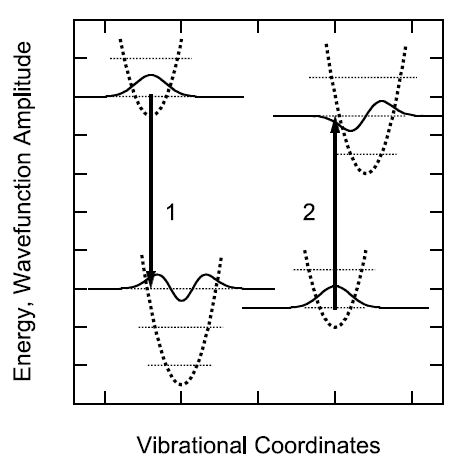
\includegraphics[width = 0.7 \textwidth]{\currfiledir/FRET.JPG}
    \caption{The resonance-energy transfer requires coupled vibronic transitions up and down. The energy lost by molecule 1 must be absorbed by molecule 2, so that the energy is maintained overall. In addition, the associated Frank-Condon factors for the transitions must be non-zero.}
\end{figure}

The total rate of energy transfer can be determined using Fermi's Golden Rule:
\begin{equation*}
    k_{rt} = \frac{2\pi}{\hbar} \cdot \int_{-\infty}^{+\infty} |H_{21}|^2 \rho_{s2}(E_1) \rho_{s1}(E_1) dE_1,
\end{equation*}
where $\rho_{si}$ denotes the state densities of molecule 1 and 2

\section{FRET on single molecules for distance measurement\protect\footnote{Parson, sections 7.2 and 7.3}} 

The strong distance dependence of FRET is used to
the relative spatial position of marker fluorophores
for example in proteins.

The transfer of energy from one excited fluorophore to another can be described with the theory of Förster resonance energy transfer. The energy transfer takes place without radiation via a dipole-dipole interaction. The rate constant $k_{rt}$ for this transition is defined as follows:
\begin{equation}
    k_{rt}=\left( \frac{9000 ln(10)\kappa^2c^4\Phi}{128\pi^5n^4N_A\tau} \right) |R_{21}|^{-6}J ,
\end{equation}
where $\kappa$ is the orientation factor, $\Phi$ and $\tau$ the quantum yield and lifetime of the donor, $R_{21}$ the distance between donor and acceptor, and J is an overlap integral between the absorption and emission spectrum of the fluorophores involved. The orientation factor $\kappa$ indicates the orientation of the two interacting partners assumed to be dipoles and can take values between $-2$ and $2$ (see Fig. \ref{KappaFactor}). 

\begin{figure}
\label{KappaFaktor}
\center
    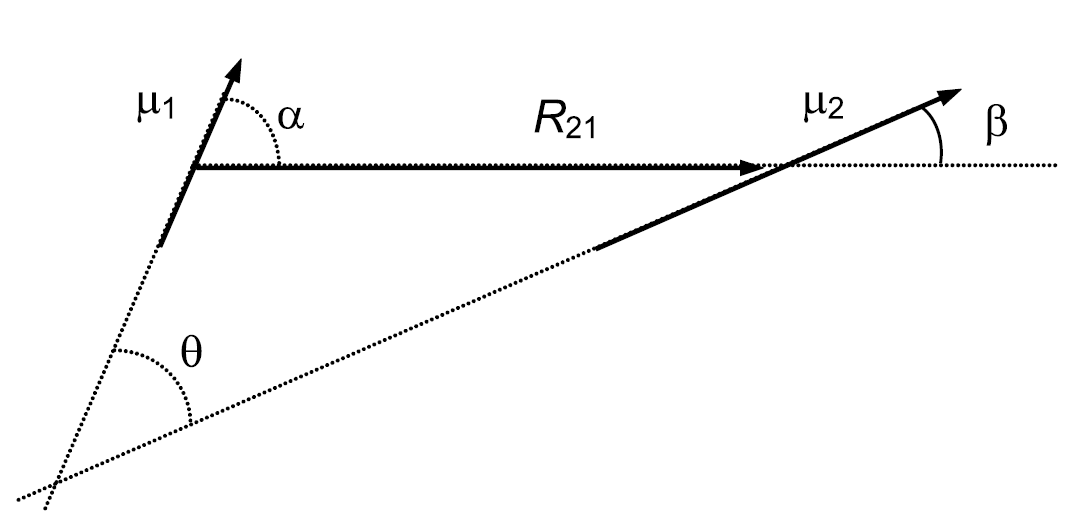
\includegraphics[width = 0.5 \textwidth]{\currfiledir/FretKappa.png}
    \caption{Sketch for the position of the angles and the distance of the dipoles. The orientation factor $\kappa$ is described by: $\kappa=\cos(\theta)-3 \cos (\alpha)\cos (\beta)$}
\end{figure}
The equation for the rate constant is also often given in the shortened form
\begin{equation}
\label{eq:fret}
    k_{rt}=\tau^{-1}(|R_{21}|/R_0)^{-6}
\end{equation}
with the forest ranger radius $R_0$. This indicates the distance at which the efficiency\footnote{The efficiency $E$ is defined as $E=\frac{1}{1+(r/R_0)^6}$ } of the energy transfer is 50\%.\par
To determine the distance between two molecules using Fret, the rate constant $k_{rt}$ must first be calculated from the fluorescence yields in the presence $\Phi$ and absence of the acceptor $\Phi_q$ using the following formula 
\[ \frac{\Phi}{\Phi_q}=1+k_{rt}\tau .\]
If the product of $k_{rt}\tau$ and the forester radius is known, the distance $|R_{21}|$ can be calculated from equation \ref{eq:fret}.




\printbibliography[segment=\therefsegment,heading=subbibliography]

%
%
%
%%
%%
%%%-------
%%
%%
%%\part{Nano-Optics and Plasmonics}
%%
%%\renewcommand{\chapterauthors}{Thorsten Schumacher}
\renewcommand{\lastmod}{April 15, 2020}

\chapter{Surface Plasmons}




\section{Tasks}

\begin{itemize}
\item T-Matrix - 2 Interfaces, M11 = 0 --> Dispersionsrelation?
Oder Winkelabhänngiges Experiment R(alpha)

\begin{tabular}{ll}
InGaAs quantum dots & \cite{Borri:2002p139}, last page  \\
CdSe nanocrystals & \cite{Jasieniak:2009er}, Fig. 2 and 3  \\
xanthene dye & \cite{Kastrup:2004p1737}, Fig. 4d   \\
MEH-PPV conjugated polymer  & \cite{Hou:2017jm}, Fig. 3 \\
LHC & ??  \\
\end{tabular}


\item Text
\item Text

\end{itemize}






%%\chapter{Overview Nano Optics}




Surface plasmons

Photonic crystals / dispersion relation

Drexhage, dipole in front of a mirror: daten vom paper

Nonlinear oscillator model, daten vom paper

TWTL: linear polarisation dependence: image analysis

Plasmon hybridisation / particle on mirror, FP probe



Plasmonic hot spots

LDOS

SHG particle symmetry


%
%-------
%
%%\nocite{*}

\printbibliography



\end{document}
